\documentclass[colortheme=yellow,txconfig=txmaths.cfg]{textbook}
\stylesetup{ 
  fullwidth-stop = catcode,
  boldemph = false,
}
\Booksetup{
  BookSeries  = 中学经典教材丛书, 
  BookTitle   = 中学数学实验教材,
  BookTitle*  = {Experimental Textbook for Middle School Mathematics},
  SubTitle    = 第四册(下),
  SubTitle*   = Volume 4B,
  BriefIntro    = 
    { },
  DedicatedTo   = 奔赴高考的莘莘学子,
  % Logo          = graphics/logo.pdf,
  CoverGraph    = graphics/4B.pdf,
  Url           = https://www.latexstudio.net,
  % ISBN          = 978-7-302-11622-6,
  Publisher     = \LaTeX 工作室出版社,
  % AuthorList*   = {David M. Stein},
  AuthorList    = {中学数学实验教材编写组},
  WrittenStyle  = 编,
  % Edition       = 9,
  % EditionStr    = 2011,
  % Price         = 188.00
}
% \usepackage{mathtools,polynom,polynomial}
\graphicspath{{figures/4B}}
\begin{document}
\frontmatter
\input{contents/maths-preface} % 基本 ok 
\tableofcontents
\mainmatter
% \input{contents/4-01.tex}
% \input{contents/4-02.tex}
% \input{contents/4-03.tex}
% \input{contents/4-04.tex}
\setcounter{chapter}{4} 
\chapter{数列和数列求和}

\section{数列的概念}
\subsection{数列的定义}

首先让我们再来看一看人类最先认识的数——自然数:$1,2,3,4,\ldots,n,n+1,\ldots$, 它们是一串依次排列的数,从 1 开始\footnote{在这套教材编写之时,0 还不被包括在自然数集之内,因此,本教材里所述的自然数实际为正整数。},逐次加 1 至无穷,这就是本节要讲的数列的一个原始的例子。下面再举几个数列的例子:

\begin{example}\label{exp:natural_number}
    在自然数里,把被 3 整除,被 3 除余 1,被 3 除余 2 的那些数,分别由小到大排列成数列。
\end{example}

\begin{solution}
    被 3 整除的数:$3,\,3\times2,\,3\times3,\,3\times4,\,\ldots,\,3n,\,3(n+1),\ldots$

被 3 除余1的数:$3+1,\,3\times2+1,\,3\times3+1,\,3\times4+1,\,\ldots,\,3n+1,\,3(n+1)+1,\,\ldots$

被 3 除余 2 的数:$3+2,\,3\times2+2,\,3\times3+2,\,3\times4+2,\,\ldots , 3n+2,\,3(n+1) +2,\,\ldots$
\end{solution}

\begin{example}\label{exp:rabbit}
  某人考察,一对兔子经过一年的繁殖,总共可以有多少对兔子,假设兔子的生殖力是这样的:每一对兔子每一个月可以生一对兔子,并且兔子在生出两个月以后就具有生殖后代的能力,在各月份里观察到的兔子的对数如下表所示:
\begin{table}
\begin{tblr}{colspec={c*{12}{X[r]}},hline{2}=0.8pt}
$n$&1&2&3&4&5&6&7&8&9&10&11&12\\
$u_n$&2&3&5&8&13&21&34&55&89&144&233&377\\
\end{tblr}
\end{table}

设 $n$ 代表月份,$u_n$ 代表该月内兔子对数。在第一个月里,第一对兔子生了一对后代,因此 $u_1=2$, 在这两对中,只有第一对能够在下一个月里生一对兔子,所以 $u_2=3$,以后各月的兔子总对数除了上一个月的兔子总对数外,再加上其中又能够在这个月产生后代的兔子对数,即前一个月的兔子的总对数,因此以后各月的兔子总对数可以由公式:
\[u_n=u_{n-1}+u_{n-2},\qquad (2< n\leqslant 12)\]
计算出来。
\end{example}

\begin{example}\label{exp:fraction}
试将 $\dfrac{1}{7}$ 准确到 $\dfrac{1}{10},\,\dfrac{1}{10^2},\,\dfrac{1}{10^3},\ldots$ 的不足近似值和过剩近似值分别排成数列。
\end{example}

\begin{solution}
  {\linespread{1.60}\selectfont
  将 $\dfrac{1}{7}$ 化成无限循环小数得到 $1/7=0.\dot{1}4285\dot{7}$. 如果分别按去尾法和进一法舍取近似数,就是说,取 $0.\dot{1}4285\dot{7}$ 前 $n$ 个数位上的数码而把它后面尾部数码都舍去,这样得到的有限小数 $u_n^-$ 叫做 $\dfrac{1}{7}$ 的准确到 $\dfrac{1}{10^n}$ 的不足近似值,而把 $u_n^+=u_n^-+\dfrac{1}{10^n}$ 叫做 $1/7$ 的准确到 $\dfrac{1}{10^n}$ 的过剩近似值。\par\medskip}

由 $\dfrac{1}{7}$ 的准确到 $\dfrac{1}{10^n}$ 的不足近似值组成的数列是
\[0.1,\; 0.14,\; 0.142,\; 0.1428,\; 0.14285,\ldots\]
由 $\dfrac{1}{7}$ 的准确到 $\dfrac{1}{10^n}$ 的过剩近似值组成的数列是
\[0.2,\; 0.15,\; 0.143,\; 0.1429,\; 0.14286,\ldots\]
显然有:
\[\begin{split}
   & 0.1<0.14<0.142<0.1428<0.14285<\cdots<\frac{1}{7}\\
   &\qquad <\cdots<
0.14286<0.1429<0.143<0.15<0.2
\end{split}\]
并且
\[\left|u_n^--\frac{1}{7} \right|<\frac{1}{10^n},\qquad \left|u_n^+-\frac{1}{7} \right|<\frac{1}{10^n}\]
\end{solution}

现在我们可以给数列下个定义如下:
\begin{Definition}
一串依次排列的数 $a_1,a_2,\ldots,a_n,\ldots$ 叫做\emph{数列}。

数列中的数,叫做数列的\emph{项},用 $a_n$ 表示,每一项的位置序数 $n$ 叫做该项的\emph{指标},通常写在 $a$ 的右下角,故也叫\emph{下标}。数列用符号 $\{a_n,\; n=1,2,3,\ldots\}$ 表示,或简写为 $\{a_n\}$。
\end{Definition}

依定义,数列就是对每一个自然数 $n$ 指定一项 $a_n$,换言之,数列就是自然数的函数。

通过前面的例子知道,我们可以用以下几种方式给出一个数列:
\begin{enumerate}
\item 给出一个以指标$n$表示数列的任意一项 $a_n$ 的公式,这公式叫做数列的\emph{通项公式}。例如在\cref{exp:natural_number} 中,数列的通项公式分别是
\[a_n=3n,\quad b_n=3n+1,\quad c_n=3n+2 \quad (n=1,2,3,\ldots)\]
\item 有的数列从某一项开始能够用在它前面的 $k$ 个项表示出来。这个表达式叫做\emph{递归方程}。例如\cref{exp:rabbit} 中的数列,由两个初始值 $u_1=2$, $u_2=3$ 和一个递归方程给出:
\[u_n=u_{n-1}+u_{n-2},\qquad (n=3,4,5,\ldots,12)\]
\item 有的数列直接用语言描述它的 $a_n$ 项,用来作一般性的讨论,如\cref{exp:fraction} 中的数列。
\end{enumerate}

\subsection{数列的种类及其定义}
\subsubsection{有穷数列和无穷数列}
有末项的数列叫做\emph{有穷数列},无末项的数列叫做\emph{无穷数列}。如\cref{exp:rabbit} 的数列是有穷数列,\cref{exp:natural_number,exp:fraction} 的数列是无穷数列。

\subsubsection{单调数列和摆动数列}

数列 $\{a_n\}$ 中的项,若满足不等式
\begin{itemize}
  \item $a_{n+1}\geqslant a_n,\quad (n=1,2,3,4,\ldots,n,\ldots)$, 那么数列叫做\emph{不减的}; 
  \item 如果 $a_{n+1}> a_n,\quad (n=1,2,3,4,\ldots,n,\ldots)$,那么数列叫做\emph{递增的};
  \item 如果 $a_{n+1}= a_n,\quad (n=1,2,3,4,\ldots,n,\ldots)$,那么数列叫做\emph{常数列};
  \item 如果 $a_{n+1}\leqslant a_n,\quad (n=1,2,3,4,\ldots,n,\ldots)$,那么数列叫做\emph{不增的};
  \item 如果 $a_{n+1}< a_n,\quad (n=1,2,3,4,\ldots,n,\ldots)$,那么数列叫\emph{递减的}。
\end{itemize}

以上各种数列统称为\emph{单调数列}。

数列 $\{a_n\}$ 中的项,如果总有一些项大于前面的项,又总有一些项小于前面的项,那么数列叫做\emph{摆动数列}。

例如:以下数列都是摆动数列
\begin{itemize}
  \item 数列 $\{(-1)^{n+1}\}$:$1,-1,1,-1,\ldots$
  \item 数列 $a_n=\begin{cases}
    \dfrac{1}{n}, & \text{$n$是奇数}\\
    \dfrac{n}{n+1}, & \text{$n$是偶数}\\
  \end{cases}$:$1,\dfrac{2}{3},\dfrac{1}{3},\dfrac{4}{5},\dfrac{1}{5},\dfrac{6}{7},\ldots$
  \item 数列 $\{(-1)^{n}n\}$:$-1,2,-3,4,\ldots$
\end{itemize}

\subsubsection{有界数列和无界数列}
有穷数列一定有最大项和最小项,无穷数列就不一定有此性质。无穷数列可分成有界数列和无界数列。

\begin{Definition}
任何一项的绝对值都小于某一正数,即 $|a_n|<M,\quad (M>0)$ 的数列叫做\emph{有界数列};没有这样正数存在的数列
叫做\emph{无界数列}。    
\end{Definition}
 
例如,数列 $\{(-1)^n\}$和$\{n+(-1)^n n\}$ 都是无界数列。

数列 $\left\{(-1)^{n+1}\left(1+\dfrac{1}{n}\right)\right\}$ 是有界数列,因为
\[|a_n|=\left|(-1)^{n+1}\left(1+\frac{1}{n}\right)\right|=1+\frac{1}{n}\leqslant 2,\quad (n=1,
2,3,4,\ldots)\]

若数列递增,并且所有 $a_n\leqslant M$(定数),则称\emph{数列有上界} $M$。

\begin{Deduction}{推论 1}
  递增有上界数列一定是有界数列。
\end{Deduction}

若数列递减,并且所有 $a_n\geqslant M$(定数),则称\emph{数列有下界} $M$。

\begin{Deduction}{推论 2}
  递减有下界数列一定是有界数列。
\end{Deduction}

\begin{Deduction}{推论 3}
  有穷数列一定是有界数列。
\end{Deduction}

图示数列的最简单的方法是直接把点 $a_1,a_2,a_3,\ldots$ 标在数轴上,这种图象可以清楚地表示数列变化的状态和趋势。\cref{fig:series_graph} 是几个数列的图象。

\begin{figure}
\begin{tikzpicture}[>=stealth]
\begin{scope}
    \draw[->] (-0.5,0)--(8,0)node[above]{$\left\{\dfrac{n}{n+1}\right\}$};
    \foreach \x/\xtext in {{1/2}/a_1, {2/3}/a_2,   {3/4}/a_3,  {4/5}/a_4}
    {
        \draw (\x*7,0)--(\x*7,.1)node[above]{$\xtext$};
    }
\foreach \x in {0,1}
{
    \draw (\x*7,0)node[below]{$\x$}--(\x*7,.1);
}
\end{scope}    
\begin{scope}[yshift=-1.5cm]
    \draw[->] (-0.5,0)--(8,0)node[above]{$\left\{\left(\dfrac{1}{2}\right)^n\right\}$};   
    \foreach \x/\xtext in {{1/2}/a_1, {1/4}/a_2,   {1/8}/a_3,  {1/16}/a_4, {1/32}/a_5}
    {
        \draw (\x*14,0)--(\x*14,.1)node[above]{$\xtext$};
    }
\foreach \x/\xtext in {0/0,1/\frac{1}{2}}
{
    \draw (\x*7,0)node[below]{$\xtext$}--(\x*7,.1);
}
\end{scope}   
\begin{scope}[yshift=-3cm]
    \draw[->] (-0.5,0)--(8,0)node[above]{$\left\{\sin n\uppi\right\}$};
    \draw (0,0)node[below]{0}--(0,.1);
    \node at (-.2,.5)[right]{$a_1=a_2=a_3=\cdots$};
\end{scope}   
\begin{scope}[yshift=-4.5cm]
    \draw[->] (-0.5,0)--(8,0)node[above]{$\left\{(-1)^n n\right\}$};
    \foreach \x/\xtext  in {-5/a_5,-3/a_3,-1/a_1,2/a_2,4/a_4}
{
    \draw (\x*.7+3.5,0)--(\x*.7+3.5,.1)node[above]{$\xtext$};
}
\foreach \x in {-1,0}
{
    \draw (\x*.7+3.5,0)node[below]{$\x$}--(\x*.7+3.5,.1);
}


\end{scope}   
\begin{scope}[yshift=-6cm]
    \draw[->] (-0.5,0)--(8,0)node[above]{$\left\{n+(-1)^n n\right\}$};
    \node at (-.2,.5)[right]{$a_1=a_3=a_5=\cdots$};
    \foreach \x/\xtext  in {0/0, 2/a_2,4/a_4,6/a_6}
{
    \draw (\x*.5,0)node[below]{$\xtext$}--(\x*.5,.1);
}
\end{scope}   
\end{tikzpicture}
    \caption{}\label{fig:series_graph}
\end{figure}
 

\begin{Exercise}
\begin{question}
  \item 自然数里的质数由小到大排成一个数列,试依次写出它的前 10 个质数。
  \item 分别用通项公式表示由小到大排列着的偶数数列和奇数数列。
  \item 试写出下列各数列的通项公式
  \begin{tasks}(2)
    \task $1^2,\; 2^2,\; 3^2,\; 4^2,\; \ldots$
    \task $1,\; -\dfrac{1}{2},\; \dfrac{1}{2}-\dfrac{1}{3},\; \dfrac{1}{3}-\dfrac{1}{4},\; \ldots$
    \task $\dfrac{3}{2},\; \dfrac{4}{3},\; \dfrac{5}{4},\; \dfrac{6}{5},\; \ldots$
    \task $\dfrac{10}{3},\; \dfrac{20}{9},\; \dfrac{30}{27},\; \dfrac{40}{81},\; \ldots$
    \task $\dfrac{1\cdot 3}{2\cdot 4},\; \dfrac{3\cdot 5}{4\cdot 6},\; \dfrac{5\cdot 7}{6\cdot 8},\; \dfrac{7\cdot 9}{8\cdot 10},\; \ldots$
    \task $1,\; -\dfrac{1}{2},\; \dfrac{1}{3},\; -\dfrac{1}{4},\; \dfrac{1}{5},\; \ldots$
    \task $1,\; 1\cdot 2,\; 1\cdot 2\cdot 3,\; 1\cdot 2\cdot 3\cdot 4,\;\ldots $
    \task $\dfrac{1}{1\cdot 2},\; -\dfrac{1}{3\cdot 4},\; \dfrac{1}{5\cdot 6},\; -\dfrac{1}{7\cdot 8},\; \ldots$
  \end{tasks}
  \item 根据下列各数列的通项公式,写出它的前 10 项。
 \begin{tasks}%(2)
    \task $a_n=\cos n\uppi,\quad (n=1,2,3,\ldots)$
    \task $a_n=\dfrac{2+(-1)^n}{n},\quad (n=1,2,3,\ldots)$
    \task $f(n)=\begin{cases}
        \dfrac{1}{n},& \text{$n$ 为奇数}\\
        \dfrac{n}{n+1},& \text{$n$ 为偶数}\\
    \end{cases}$
\end{tasks}       

\item 试将所有整数排成一个数列,并且用通项公式表示出来。
\item 数列的通项公式是
\[f(n)=\frac{5+3\sqrt{5}}{10}\left(\frac{1+\sqrt{5}}{2}\right)^n+\frac{5-3\sqrt{5}}{10}\left(\frac{1-\sqrt{5}}{2}\right)^n,\quad (n=1,2,3,\ldots)\]
\begin{tasks}
  \task 求 $f(1)$, $f(2)$;
  \task 求证 $f(n)=f(n-1)+f(n-2)$.
\end{tasks}

\item 判断下列各数列的类型并图示它前 5 项。
\begin{tasks}
  \task $a_n=1-2n,\quad (n=1,2,3,\ldots,10)$;
  \task $a_n=\dfrac{2n+1}{n},\quad (n=1,2,3,\ldots)$;
  \task $a_n=\dfrac{(-1)^n2^n}{4},\quad (n=1,2,\ldots,5)$;
  \task! $a_n=\dfrac{(-1)^{n+1}n}{n+1},\quad (n=1,2,3,\ldots)$;
  \task* $\sqrt{2}$ 的准确到 $1,\; 0.1,\; 0.01,\; \ldots$ 的过剩近似值。
  \task* $a_n=\dfrac{2+(-1)^n}{n},\quad (n=1,2,3,\ldots)$;
  \task* $a_n=(-1)^n\left(\dfrac{n-1}{n+1}\right)^2,\quad (n=1,2,3,\ldots)$;
  \task $a_n=\dfrac{2n^2-3}{n},\quad (n=1,2,3,\ldots)$;
  \task $a_n=\dfrac{-2n^2-3}{n},\quad (n=1,2,3,\ldots)$;
  \task $a_n=\tan \dfrac{n\uppi}{3},\quad  (n=1,2,3,\ldots)$。
\end{tasks}
\item 数列的通项公式是
\[a_n=2n^2-3,\quad (n=1,2,3,\ldots)\]
求数列的第 5 项,下面三个数:84788、32352 和 72197中,哪个数是数列中的项,是第几项?
\end{question}
\end{Exercise}

\section{数列求和举例}
在本节,我们要复习第一册已经学习过的两个简单而重要的数列,即等差数列和等比数列,同时通过例题来说明几种常用的求数列前 $n$ 项和的方法。

如果一个数列,从第二项起,每一项减去它的前面的一项所得的差都等于同一个常数,那么这个数列叫做\emph{等差数列},这个常数叫做等差数列的\emph{公差},用符号 $d$ 表示。等差数列的通项公式是
\[a_n=a_1+(n-1)d,\qquad (n=1,2,3,\ldots)\]
它的前 $n$ 项求和公式是
\[S_n=\frac{n(a_1+a_n)}{2}\]
或
\[S_n=na_1+\frac{n(n-1)}{2}d\]
我们已在第一册给出上面求和公式的推导过程,现在建议读者独立地把它们推导出来,在通项公式与求和公式中共包含了五个数量:$a_1$, $d$, $n$, $a_n$ 和 $S_n$。如果问题给出了其中三个数量,那么其余两个数量便可由它们解出来。

\begin{example}
  在数轴上有两个点 $A(4.5)$ 和 $B(12.5)$,在其间插入四个等间隔的点,求这些点的坐标。
\end{example}

\begin{solution}
  在 $A$ 和 $B$ 两点之间插入四个等间隔的点后,这六个点的对应坐标成等差数列,

$\because\quad     a_1=4.5,\quad a_6=12.5,\quad n=6$

$\therefore\quad     12.5=4.5+(6-1)d$,解得:$d=1.6$。

所求四个点的坐标分别是 $6.1,\; 7.7,\; 9.3,\; 10.9$。
\end{solution}

\begin{Definition}
  给出两个数,其间插入一个数,使成等差数列,被插入的数叫做这二数的\emph{等差中项}。
\end{Definition}

\begin{Deduction}{推论}
  若 $a,b,c$ 三个数成等差数列,则等差中项 \[b=\frac{a+c}{2}\]
\end{Deduction}
 
事实上,依定义有
\[b-a=c-b\]
移项,得
\[2b=a+c\]
即
\[b=\frac{a+c}{2}\]
    
\begin{example}
  在甲地有 48 根电杆,从离甲地 1000 米的地方树立第一根电杆,以后每隔 15 米树立一根电杆,载重汽车每次只能拖运三根电杆,问由一辆汽车去完成任务至少需要行驶多少公里?
\end{example}

\begin{solution}
  汽车需运电杆 $48\div 3=16$ 次才能完成任务,所以,$n=16$。设 $a_n$ 为第 $n$ 次拖运电杆再返回原地所行驶的路程,依题意 $\{a_n\}$ 是等差数列,且知 
\[    a1=2060,\qquad d=90,\qquad n=16\]
因此:
\[\begin{split}
    S_n&=na_1+\frac{n(n-1)}{2}d\\
    &=16\times 2060+\frac{16\times 15}{2}\times 90\\
    &=43760\,\unit{(\text{米})}=43.76\,\unit{(\text{公里})}
\end{split}\]

答:汽车需行驶 43.76 公里,才能完成任务。
\end{solution}

\bigskip
如果一个数列,从第二项起,每一项和前面一项的比都等于一个常数,那么,这个数列叫做\emph{等比数列}。这个常数叫做等比数列的\emph{公比},通常用字母 $q$ 表示。换言之,等比数列是满足递归关系 $a_{n+1}=qa_{n},\quad (n=1,2,\ldots)$ 的数列。

显然,当 $q>0$ 时,等比数列是单调的。若 $q>1$,等比数列是递增的;若 $0<q<1$,等比数列是递减的;若 $q=1$,等比数列是常数列。

当 $q<0$ 时,等比数列是摆动的。

又当 $|q|\leqslant 1$ 时,等比数列是有界的,当 $|q|>1$ 时,等比数列是无界的。

我们已经知道等比数列的通项公式是
\[a_n=a_1q^{n-1}\qquad (n=1,2,\ldots)\]
它前 $n$ 项和公式是
\[S_n=\frac{a_nq-a_1}{q-1}\]
若 $q<1$,上式改写为
\[S_n=\frac{a_1-a_nq}{1-q}\]
显然,若 $q=1$,则 $S_n=na_1$。

将 $a_n=a_1q^{n-1}$ 代入求和公式中,得到
\[S_n=\frac{a_1(q^n-1)}{q-1}\]

\begin{Definition}
  任给两个数,在其间插入一个数,使成等比数列,则所插入的数叫做所给两数的\emph{等比中项}。
\end{Definition}

\begin{Deduction}{推论}
  若 $a,b,c$ 三个数成等比数列,则等比中项 $b=\pm\sqrt{ac}$,(或 $b^2=ac$)。    
\end{Deduction}

事实上,依定义有
\[\frac{b}{a}=\frac{c}{b}\]
因此:$b^2=ac$,或者$b=\pm\sqrt{ac}$。

\begin{example}
  在 81 和 1 之间,插入三个实数,使它们和这两个数成等比数列。
\end{example}

\begin{solution}
  在 81 和1之间,插入三个数后,1 就成为等比数列的第 5 项,因此
\[\begin{split}
  a_5=81q^4&=1\\
  (9q^2+1)(9q^2-1)&=0  
\end{split}\]
$\because\quad q$ 为实数,$\therefore\quad 9q^2+1\ne 0$,由此得:
\[9q^2-1=0\quad \Rightarrow\quad q=\pm\frac{1}{3}\]
故所求三个实数为 $27,9,3$ 或 $-27,9,-3$。
\end{solution}


\begin{example}
  已知一个正三角形,边长为 $a$,以此正三角形的高线为边做第二个三角形,依此类推,求前 10 个正三角形的面积的和。
\end{example}

\begin{figure}
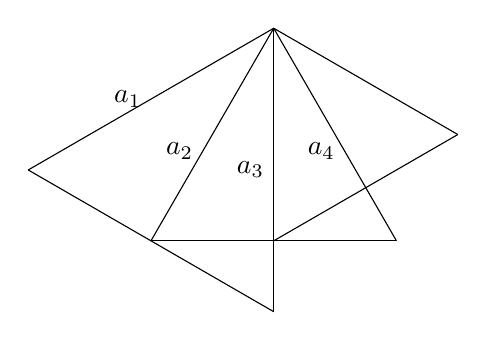
\begin{tikzpicture}[scale=1.8,]
    \foreach \x/\xlen in {-150/2, -120/1.732, -90/2, -60/1.732, -30/1.5}
    {
        \draw(0,0)--(\x:\xlen);
    }
\draw (-150:2)--(-90:2); 
\draw (-120:1.732)--(-60:1.732); 
\draw (-90:1.5)--(-30:1.5); 

\foreach \x in {1,2,3,4}
{
    \node at (-180+30*\x:1)[left]{$a_{\x}$};
}
\end{tikzpicture}
    \caption{}\label{fig:triangle}
\end{figure}


\begin{solution}
  如\cref{fig:triangle},设第 $k$ 个这样的正三角形的边长为 $a_k$,高为 $h_k$, 面积为 $A_k,\; (k=1,2,\ldots,10)$,于是
\[a_1=a,\qquad h_1=\frac{\sqrt{3}}{2}a,\qquad A_1=\frac{1}{2}a_1h_1=\frac{\sqrt{3}}{4}a^2\]
因为所有正三角形都相似,故对应边与对应高线成比例,即
\[\frac{a_{k+1}}{a_{k}}=\frac{h_{k+1}}{h_k}\]
又依三角形的作法,知
\[a_{k+1}=h_k,\qquad (k=1,2,3,\ldots,10)\]
\[\therefore\quad \frac{a_{k+1}}{a_{k}}=\frac{h_{k+1}}{a_{k+1}}=\frac{h_1}{a_1}=\frac{\sqrt{3}}{2}\]
根据相似三角形面积之比等于对应边平方之比,故
\[q=\frac{A_{k+1}}{A_k}=\frac{a^2_{k+1}}{a^2_k}=\left(\frac{a_{k+1}}{a_k}\right)^2=\left(\frac{\sqrt{3}}{2}\right)^2=\frac{3}{4}\]
因此,前 10 个正三角形面积之和
\[S_{10}=\frac{\dfrac{\sqrt{3}}{4}a^2\left[1-\left(\dfrac{3}{4}\right)^{10}\right]}{1-\dfrac{3}{4}}=\sqrt{3}a^2\left[1-\left(\frac{3}{4}\right)^{10}\right]\]
\end{solution}

{\linespread{1.65}\selectfont 为书写简便起见,我们用符号 $\sum\limits^n_{i=m}a_i$ 表示数列 $\{a_i\}$ 的相邻的一些项的和。整数 $i$ 在确定了的界限内变动,在 $\sum$ 的下面和上面的数字分别表示求和的起止项的序号,符号“$\sum$”读作 sigma。例如\par}
\[\begin{split}
    \sum^n_{i=1}a_i&=a_1+a_2+\cdots+a_n\\
    \sum^n_{i=k}a_i&=a_k+a_{k+1}+\cdots+a_n\\
\end{split}\]

在许多数学问题里,我们需要求出以下标 $i$ 的 $k$ 次多项式 $f(i)$ 为通项的前 $n$ 项和的公式:
\[S_k(n)=\sum^{n-1}_{i=0}f(i)=f(0)+f(1)+\cdots+f(n-1)\]
这里的指标集是非负整数集。

数列 $\{S_k(n)\}$ 称为数列 $\{f(n)\}$ 的和数列,即
\[\begin{split}
    S_k(1)&=f(0)\\
    S_k(2)&=f(0)+f(1)\\
    S_k(3)&=f(0)+f(1)+f(2)\\
    \cdots
\end{split}\]

为讨论方便起见,规定 $S_k(0)=0$, 于是和数列 $\{S_k(n)\}$ 满足下面两个性质:
\begin{enumerate}[itemindent=3.5em]
    \item $S_k(0)=0$
    \item $S_k(n+1)-S_k(n)=f(n),\qquad n=0,1,2,\ldots$
\end{enumerate}

我们来考虑这样一个多项式,它在 $k$ 个点 $0,1,2,\ldots,k-1$ 处与横坐标轴相交,又通过 $(k,1)$ 点,显然这个关于 $n$ 的多项式为
\[q_k(n)=\frac{n(n-1)\cdots(n-k+1)}{k!}\]
下面来求数列 $\{q_k(n)\},\; n=0,1,2,\ldots$ 的前 $n$ 项和的公式。

\begin{example}\label{exp:sum_of_qk}
设 $q_k(n)=\dfrac{1}{k!}n(n-1)\cdots(n-k+1)$,则前 $n$ 项的和
\[\begin{split}
    S_k(n)&=\sum^{n-1}_{i=0} q_k(i)=q_k(0)+q_k(1)+\cdots+q_k(n-1)\\
    &=\frac{1}{(k+1)!}n(n-1)\cdots(n-k)
\end{split}\]
换言之,其和是这样一个多项式,它在 $0,1,2,\ldots,(k-1)$,共 $k$ 个点处与坐标轴相交且通过 $((k+1),1)$ 点。
\end{example}

\begin{solution}
设 $S_k(n)$是一个 $n$ 的 $k+1$ 次多项式,且让 $S_k(n)$ 满
足条件:
\begin{align}
    \label{eq:Skn}S_k(0)&=0\\
    \label{eq:Skn+1}S_k(n+1)-S_k(n)&=q_k(n)
\end{align}
由于 $q_k(0)=q_k(1)=\cdots=q_k(k-1)=0$,且 $q_k(k)=1$,于是
\begin{equation}
    \begin{split}
 S_k(n)&=q_k(0)+q_k(1)+\cdots+q_k(n-1)\\
&=\underbrace{0+0+\cdots+0}_{\text{$k$项}}+1+(k+1)+\\
&\qquad \cdots+
\frac{1}{k!}(n-1)(n-2)\cdots(n-k)     
    \end{split}
\end{equation}

由\cref{eq:Skn,eq:Skn+1} 得到
\begin{align}
S_k(0)=S_k(1)=\cdots=S_k(k)=0\\
\label{eq:Skk+1}S_k(k+1)=1
\end{align}
从而知道 $S_k(n)$ 有下面 $k+1$ 个因式,即
\[S_k(n)=Cn(n-1)(n-2)\cdots(n-k)\]
这里 $C$ 是未定的常数因子。

常数因子 $C$ 可由\cref{eq:Skk+1} 确定,
\[S_k(k+1)=C(k+1)k(k-1)\cdots2\cdot 1=1\]
\[\therefore\quad C=\frac{1}{(k+1)!}\]

此处记 $(k+1)!=1\cdot 2\cdot 3\cdots k(k+1)$。

因此,
\[\begin{split}
    S_k(n)&=\sum^{n-1}_{i=0} q_k(i)=\sum^{n-1}_{i=0} \frac{1}{k!}i(i-1)\cdots (i-k+1)\\
    &=\frac{1}{(k+1)!}n(n-1)\cdots (n-k)
\end{split}\]
\end{solution}

我们也常用这样一种想法来求数列前 $n$ 项和的公式,即如果数列的通项能分解成另一个数列相邻两项的差:

$f(n)=F(n+1)-F(n),\; n=0,1,2,\ldots$时,那么前 $n$ 项的和
\[\begin{split}
   S(n)&= \sum^{n-1}_{i=0} f(i)= \sum^{n-1}_{i=0} [F(i+1)-F(i)]\\
   &=[F(1)-F(0)]+[F(2)-F(1)]+\cdots +[F(n)-F(n-1)]\\
   &=F(n)-F(0)
\end{split}\]


\begin{example}
    求 $S(n)=\dfrac{1}{1\cdot 4}+\dfrac{1}{4\cdot 7}+\dfrac{1}{7\cdot 10}+\cdots +\dfrac{1}{(3n-2)(3n+1)}$ 的和。
\end{example}

\begin{solution}
$\because\quad \dfrac{1}{(3i-2)(3i+1)}=\dfrac{1}{3}\left(\dfrac{1}{3i-2}-\dfrac{1}{3i+1}\right)$

\bigskip 当 $i=1,2,3,\ldots,n$ 时,有
\[\begin{split}
    \frac{1}{1\cdot 4}&=\frac{1}{3}\left(\frac{1}{1}-\frac{1}{4}\right)\\
    \frac{1}{4\cdot 7}&=\frac{1}{3}\left(\frac{1}{4}-\frac{1}{7}\right)\\
    \cdots &\cdots\\
    \frac{1}{(3n-2)(3n+1)}&=\frac{1}{3}\left(\frac{1}{3n-2}-\frac{1}{3n+1}\right)
\end{split}\]
因此:
\[\begin{split}
    S(n)&=\sum^n_{i=1}\frac{1}{(3i-2)(3i+1)}\\
    &=\frac{1}{3}\left(\frac{1}{1}-\frac{1}{3n+1}\right)\\
    &=\frac{n}{3n+1}
\end{split}\]
\end{solution}

如果数列的通项是以其它形式的 $k$ 次多项式给出的,我们可以用待定系数法把它变形为\cref{exp:sum_of_qk} 的形式。


\begin{example}
  求 $S_2(n+1)=0^2+1^2+2^2+\cdots+n^2$ 的和。
\end{example}

\begin{solution}
  设 $i^2=\lambda \dfrac{i(i-1)}{2!}+\mu i,\; (i=0,1,2,\ldots,n)$,由待定系数法求得:
\[\lambda=2,\qquad \mu=1\]
于是:
\[S_2(n+1)=\sum^n_{i=0}i^2=2\sum^n_{i=0}\frac{i(i-1)}{2!}+\sum^n_{i=0}i\]
应用\cref{exp:sum_of_qk} 的结果,得到:
\[\begin{split}
    S_2(n+1)&=2\frac{(n+1)n(n-1)}{3!}+\frac{n(n+1)}{2}\\
    &=\frac{n(n+1)(2n+1)}{6}
\end{split}\]
\end{solution}

\begin{example}
设 $a_0,a_1,a_2,\ldots,a_n$ 成等差数列,求 $S_n=a_0+a_1x+a_2x^2+a_3x^3+\cdots+a_nx^n$ 的和。    
\end{example}

\begin{solution}
  \begin{equation}
    \label{eq:sum_anxn}
    S_n=a_0+a_1x+a_2x^2+a_3x^3+\cdots+a_nx^n
  \end{equation}
由于\cref{eq:sum_anxn} 中的系数成等差数列,变量 $1,x,x^2,\ldots,x^n$ 成等比数列,利用等差数列的任意相邻的三项有递归关系:
\begin{equation}
    a_n-2a_{n-1}+a_{n-2}=0,\qquad n\geqslant 2
\end{equation}
知道\cref{eq:sum_anxn} 相邻的三项下面等式成立:
\begin{equation}
  \label{eq:zero_item}
  a_nx^n-2x(a_{n-1}x^{n-1})+x^2(a_{n-2}x^{n-2})=0,\qquad n\geqslant 2
\end{equation}
让\cref{eq:sum_anxn} 的两边分别乘以 $1,-2x,x^2$, 然后相加,得
\[\begin{split}
    S_n&=a_0+a_1x+a_2x^2+a_3x^3+\cdots+a_{n-1}x^{n-1}+a_nx^n\\
    -2xS_n&=-2a_0x-2a_1x^2-2a_2x^3-\cdots-2a_{n-1}x^n-2a_nx^{n+1}\\
    x^2S_n&=a_0x^2+a_1x^3+a_2x^4+\cdots+a_{n-1}x^{n+1}+a_nx^{n+2}
\end{split}\]
所以:
\[(1-x)^2 S_n=a_0+(a_1-2a_0)x+0+\cdots+0+(a_{n-1}-2a_n)x^{n+1}+a_nx^{n+2}\]
由\cref{eq:zero_item} 可知在上面等式中,其余各项为 0,若 $x\neq 1$,两边除以 $(1-x)^2$,得
\[S_n=\frac{a_0+(a_1-2a_0)x+0+\cdots+0+(a_{n-1}-2a_n)x^{n+1}+a_nx^{n+2}}{(1-x)^2}\]
若 $x=1$,原题就变成求等差数列前 $n$ 项的和,这时,
\[S_n=\frac{n(a_1+a_n)}{2}\]
\end{solution}

\begin{example}
    数列 $\{v_n\}$ 由下面递归定义给出:
 \[ v_{n+1}=3v_n-2v_{n-1},\quad v_0=2,\quad v_1=3,\; n=1,2,3,\ldots\]
 求:$v_n$,$S_n=\sum\limits^{n-1}_{i=0}v_i$。
\end{example}

\begin{solution}
    由 $v_{n+1}=3v_n-2v_{n-1}$ 容易看出
  \[  v_{n+1}-v_{n}=2(v_n-v_{n-1})\]
    设 $q_n=v_{n+1}-v_n$,$q_{n-1}=v_n-v_{n-1}$, 则 $q_n=2q_{n-1},\; (n=1,2,\ldots)$,换言之,$\{q_n\}$ 是公比为 2 的等比数列,
\[\therefore\quad q_n=2q_{n-1}=2^2q_{n-2}=\cdots=2^n(v_1-v_0)=2^n(3-2)=2^n\]
从而:
\[\begin{split}
    q_{n-1}&=v_n-v_{n-1}=2^{n-1}\\
v_n&=(v_n-v_{n-1})+(v_{n-1}-v_{n-2})+\cdots+(v_1-v_0)+v_0\\
&=2^{n-1}+2^{n-2}+\cdots +2+1+2\\
&=(2^n-1)+2=2^n+1\\
\end{split}\]
\[\begin{split}
    S_n=\sum^{n-1}_{i=0}v_i&=\sum^{n-1}_{i=0}(2^i+1)=\sum^{n-1}_{i=0}2^i+\sum^{n-1}_{i=0}1\\
    % &=\sum^{n-1}_{i=0}2^i+\sum^{n-1}_{i=0}1\\
    &=(2^n-1)+n=2^n+(n-1)
\end{split}\]
\end{solution}

\begin{Exercise}
\begin{question}
  \item 在等差数列中
  \begin{tasks}(2)
    \task 若 $a_5=100$, $d=\frac{1}{2}$,求$a_{100}$;
    \task 若 $a_3=-4$, $a_5=2$, 求 $a_{10}$;
    \task 若 $a_p=q$, $a_q=p$, 求 $a_{p+q}$;
    \task 用 $a_s$, $a_1$, $d$ 表示 $a_n$。
  \end{tasks}

\item 在 7 和 35 之间插入 6 个数使它们和已给两数组成等差数列。
\item 在 8 和 32 之间应插入多少个等差中项,可使等差中项中的前两个数的和与后两个数的和之比为 $7:25$。
\item 求证含有奇数个项的等差数列里,第一项,中间项,最后项也成等差数列。
\item 在三位数里有几个是 6 的倍数,求它们的和。
\item 求 $S_n=1-2+3-4+5-\cdots+(-1)^{n+1}n$ 的和。
\item 一等差数列前 $n$ 项之和为 $S_n=5n^2+3n$,求 $a_n$。
\item 在等差数列中
\begin{tasks}
  \task 已知 $d=2$, $n=15$, $a_{15}=-10$, 求 $S_{15}$;
  \task 已知 $a_n$, $S_n$ 和 $a_1$,求 $d$;
  \task 已知 $d$, $S_n$ 和 $a_1$,求 $n$;
  \task 已知 $a_n$, $S_n$ 和 $d$, 求 $a_1$。
\end{tasks}

\item 求等差数列 $2\dfrac{1}{2},1\dfrac{5}{6},1\dfrac{1}{6},\ldots$ 的第 $n$ 项,并求这个等差级数的最大和。

\bigskip
\item 在等差数列中,若 $S_1=a_1+a_3+\cdots+a_{2n-1}=44$,$S_2=a_2+a_4+\cdots+a_{2n-2}=33$,求 $a_n$。
\item 某化工厂为了加固烟囱,要在烟囱上打 32 道铁箍,且使每两道铁箍之间的距离相等,已知最上面一道铁箍处烟囱的外直径为 \qty{1.5}{m},最下面一道箍处烟囱的外直径为 \qty{3.5}{m}。求全部铁箍用料的总长。

\item 若 $a_1,a_2,\ldots,a_n$ 成等差数列,求证:
\[\frac{1}{\sqrt{a_1}+\sqrt{a_2}}+\frac{1}{\sqrt{a_2}+\sqrt{a_3}}+\cdots +\frac{1}{\sqrt{a_{n-1}}+\sqrt{a_n}}=\frac{n-1}{\sqrt{a_1}+\sqrt{a_n}}\]

\item 求下列各等比数列的通项公式
\begin{tasks}(2)
    \task $-1,\;-2,\;-4,\;\ldots$
    \task $-1,\;1,\;-1,\;\ldots$
    \task $\dfrac{2}{3},\;\dfrac{1}{2},\;\dfrac{3}{8},\;\ldots$
    \task $\sqrt{2},\;1,\;\dfrac{\sqrt{2}}{2},\;\ldots$
    \task $1,\;-\sqrt{\dfrac{1}{3}},\;\dfrac{1}{3},\;\ldots$
\end{tasks}

\item 在等比数列里
\begin{tasks}
  \task $a_1=36$, $a_5=2\dfrac{1}{4}$,求 $q$ 和 $S_5$;
  \task $a_n=1296$, $q=6$, $S_n=625$,求 $a_0$ 和 $a_1$;
  \task $a_1=3$, $q=\dfrac{1}{3}$, $n=8$,求 $S_8$;
  \task $S_5=242$, $q=3$,求 $a_5$。
\end{tasks}
\item 在等比数列里,若 $a_7-a_5=a_6+a_5=48$, 求 $a_1$, $q$ 和 $S_{10}$。
\item 在 160 和 5 之间插入 4 个数,使这 6 个数成等比数列,求这 4 个数。
\item 求证,若 $a_1,a_2,\ldots,a_n,\ldots\; (a_i>0,i=1,2,3,\ldots)$ 成等比数列,则以下数列均成等比数列:
\begin{tasks}(2)
  \task $a_1,\; a_3,\; \ldots, a_{2n-1},\; \ldots$;
  \task $ka_1,\; ka_3,\; \ldots, ka_{2n-1},\; \ldots$;
  \task $\dfrac{1}{a_1},\; \dfrac{1}{a_2},\; \ldots, \dfrac{1}{a_{n}},\; \ldots$;
  \task $a^2_1,\; a^2_2,\; \ldots, a^2_{n},\; \ldots$;
  \task $\sqrt{a_1},\; \sqrt{a_2},\; \ldots, \sqrt{a_n},\; \ldots$。
\end{tasks}

\item 从盛满 \qty{20}{L} 纯酒精的容器里倒出 \qty{1}{L},然后用水填满,再倒出 \qty{1}{L} 混合溶液,用水填满,这样继续进行,一共倒三次,这时容器里有纯酒精多少?
\item 甲厂产量是乙厂产量的 40.96\%,甲厂产品每年增长的百分率比乙厂产品每年增长的百分率多 30\%,若第四年甲厂产量和乙厂产量相同,求甲厂每年产品平均增长的百分率是多少?
\item 一个机器制造厂的原订的三年计划,每年比上一年增产的机器台数相同,但到了第三年,由于实际需要,须比原计划多生产 1000 台,那么每年比上一年的增长百分数就相同,而且第三年的台数恰为原计划总台数的一半,问实际上每年生产了多少台?每年比上一年增长的百分数是多少?
\item 某农机厂去年十月份生产拖拉机 1000 台,这样连同一月至九月的产量恰好完成全年生产任务,为加速农业机械化,全厂在年底前又生产了 2310 台,于是就超额完成全年计划的 21\%。求
\begin{tasks}
  \task 今年十一、十二月份每月平均增长率;
  \task 今年原计划生产量。
\end{tasks}

\item 若一个三角形的三个角成等差数列,而它的边成等比数列,求这个三角形的形状。
\item 已知一个正三角形边长为 $a$,以此正三角形的高线为边做第二个三角形,依此类推,求前 10 个正三角形的周长的和。
\item 求 $(x+y)+(x^2+xy+y^2)+(x^3+x^2y+xy^2+y^3)+\cdots$ 的前 $n$ 项的和。
\item 求 $7+77+777+\cdots$ 的前 $n$ 项的和。
\item 设等比数列 $a_1,a_2,\ldots,a_n,\ldots$ 的公比是 $q$。求证:$a_1a_2\cdots a_n=a^n_1q^{\tfrac{n(n-1)}{2}}$

\item 求下列各数列的和
\begin{tasks}(3)
    \task $\displaystyle \sum^{n-1}_{i=0} i^3$
    \task $\displaystyle \sum^{n-1}_{i=0} i^4$
    \task $\displaystyle \sum^{n-1}_{i=0} (i-1)i$
    \task $\displaystyle \sum^{n-1}_{i=0} (2i-1)^2$
    \task $\displaystyle \sum^{n-1}_{i=0} \frac{2i+1}{i^2\cdot (i+1)^2}$
\end{tasks}

\item 数列 $a_0,a_1,\ldots, a_n,\ldots$ 中的 $a_0,a_1$ 为已知,且 $a_n=\dfrac{a_{n-1}+a_{n-2}}{2},\; n=2,3,4,\ldots$,求 $a_n$。
\item 数列 $a_1,a_2,\ldots,a_n,\ldots$中,$a_1=2$,且$a_n=3a_{n-1}+1\; (n=2,3,4,\ldots )$, 求 $a_1+a_2+\cdots +a_n$。
\item 已知数列 $a_1,a_2,\ldots ,a_n,\ldots$ 的相邻两项 $a_n$,
$a_{n+1}$ 是方程 $x^2+3nx+c_n=0,\; (n=1,2,\ldots)$ 的两根,当 $a_1=1$ 时,求 $\sum\limits^{2p}_{n=1}c_n$。
\item $n$ 是非负的整数,试问同时满足下面三个不等式的整数对 $(x,y)$ 共有多少组?
\[y\geqslant x,\qquad y\leqslant 3x,\qquad y\leqslant n\]
\item 三角形三条边的长分别是$\ell$, $m$ 和 $n$,这里 $\ell$,$m$,
$n$都是正整数,且$\ell\leqslant m\leqslant n$,对于每一个给定的$n$(取
$n=1,2,3,\ldots$),所说的不同形状的三角形有多少个?求
出三角形的个数用 $n$ 表示的一般公式。
\item 数列 $\{a_n\}$ 是:
\[a_1=\frac{1}{3},\qquad \frac{1}{a_{n+1}}-\frac{1}{a_n}=2n+3\quad (n=1,2,3,4,\ldots)\]
\begin{tasks}
  \task 用 3 的式子表示一般项;
  \task 用 $n$ 的式子表示前 $n$ 项的和 $\displaystyle\sum^n_{k=1}a_k$
\end{tasks}

\item 若数列 $\{a_n\}$ 是等差数列,
求证:\[\frac{1}{a_1a_2}+\frac{1}{a_2a_3}+\cdots+\frac{1}{a_{n-1}a_n}=\frac{n-1}{a_1a_n}\]
\end{question}
\end{Exercise}

\section{数学归纳法}
现在我们研究在数学中常用的一种证明方法——数学归纳法。

我们常常从一些特殊事实归纳出一般结论,这种推理方法就是通常说的归纳法,用归纳法可以帮助我们从特殊情况发现一般规律,但如果归纳时所根据的特殊事实没有完全包括结论中所涉及到的所有情况,结论可能不正确,这就是说:命题可能对于一系列的特别情形是对的,但是一般并不正确。

例如,已知函数 $f(n)=(n^2-5n+5)^2$,则
\[f(1)=1,\qquad f(2)=1,\qquad f(3)=1,\qquad f(4)=1 \]
如果我们由此得出结论 $f(n)=(n^2-5n+5)^2=1$ ($n$ 是任何自然数),那就是错误的,事实上,$f(5)=25$,不等于1。

为了克服这种归纳法的不完全性,我们常采用下述的数学归纳法来证明一个关于自然数 $n$ 的命题。

数学归纳法的证明逻辑是:

对于一个依赖于自然数 $n=1,2,3,\ldots$ 的命题 $p(n)$,如果
\begin{enumerate}
  \item 当 $n=1$ 时,命题 $p(1)$ 正确;
  \item 假设 $n=k,\; (k\geqslant 1)$ 时,命题 $p(k)$ 正确,可以推出 $n=k+1$ 时,命题 $p(k+1)$ 正确,那么,命题 $p(n)$ 对于一切自然数 $n=1,2,3,\ldots$ 都正确。
\end{enumerate}

这个方法的根据,就是自然数的基本性质:

\begin{Theorem}[自然数的基本性质]{性质}
  令 $A$ 是自然数集 $\mathbb{N}$ 中具有下面性质的子集:
\begin{enumerate}
  \item\label{itm:prop1} $1\in A$;
  \item\label{itm:prop2} 若 $n\in A$,则 $n+1\in A$
\end{enumerate}
那么:$A=\mathbb{N}$。
\end{Theorem}

现在,我们来证明数学归纳法的正确性,设使命题 $p(n)$ 成立的自然数是自然数集 $\mathbb{N}$ 中的子集 $A$,即 $A\subseteq \mathbb{N}$。

根据数学归纳法中的 \ref{itm:prop1},$1\in A$; 再根据数学归纳法中的 \ref{itm:prop2},若 $n\in A$,则 $n+1\in A$。于是,根据自然数的基本性质,得到
\[A=\mathbb{N}\]
因此,命题 $p(n)$ 对于一切自然数成立。

下面举一些例子说明这个方法的应用。

\begin{example}
  求证:
  \begin{equation}
    \label{eq:sum_n}
    1+2+3+\cdots+n=\frac{n(n+1)}{2}
  \end{equation}
\end{example}

\begin{analyze}
    我们注意到和式:$1+2+3+\cdots+n$ 可以递归地定义为
\[\begin{cases}
    S(1)=1\\
    S(n)=S(n-1)+n,\qquad n=2,3,\ldots
\end{cases}\]
上面的等式为应用数学归纳法去证明打下了基础。
\end{analyze}

\begin{proof}
  \begin{enumerate}
    \item\label{itm:proof1} 当 $n=1$ 时,$\because\, S(1)=1,\quad \dfrac{1\times(1+1)}{2}=1$,$\therefore\, $ \cref{eq:sum_n} 成立。
    \item\label{itm:proof2} 假设 $n=k,\; (k\geqslant 1)$ 时,\cref{eq:sum_n} 成立,即有
\[S(k)=1+2+3+\cdots+k=\frac{k(k+1)}{2}\]
那么,当 $n=k+1$ 时,
\[S(k+1)=1+2+3+\cdots+k+(k+1)=S(k)+(k+1)\]
应用数学归纳法假设于上面的等式,得到
\[\begin{split}
    S(k+1)&=\frac{k(k+1)}{2}+(k+1)=(k+1)\left(\frac{k}{2}+1\right)\\
    &=\frac{(k+1)(k+2)}{2}\\
    &=\frac{(k+1)[(k+1)+1]}{2}
\end{split}\]
即\cref{eq:sum_n} 仍成立。

由所证 \ref{itm:proof1} 和 \ref{itm:proof2} 两步知:
\[1+2+3+\cdots+n=\frac{n(n+1)}{2}\]
对于一切自然数 $n$ 都成立。
\end{enumerate}
\end{proof}

从上例明显地看出,用数学归纳法证明一个命题的步骤是:
\begin{enumerate}
\item\label{itm:stp1} 验证命题 $p(n)$,当 $n$ 取第一个值 $n=1$ 时,$p(1)$ 正
确。这一条是数学归纳法的基础。
\item\label{itm:stp2} 假设当 $n=k,\; (k\geqslant 1)$时,命题 $p(k)$ 正确,证明当 $n=k+1$ 时,命题 $p(k+1)$ 也正确。这一条是说性质 $p(n)$ 具有遗传性,可以一代一代地传下去。完成了这两步以后,就可以断定命题 $p(n)$ 对于一切自然数 $n$ 都正确。因为首先证明 $p(1)$ 正确,另外由 $p(1)$ 正确推出 $p(2)$ 正确,由 $p(2)$ 正确推出了 $p(3)$ 正确,依次下去,便可知对于一切自然数 $n$,$p(n)$ 正确。
\end{enumerate}


有时不一定从 1 开始,也就是数学归纳法里两句话,可以改成
\begin{enumerate}
  \item 当 $n=k_0$ 时,命题 $p(k_0)$ 正确。
  \item 从假设 $n=k,\; (k\geqslant k_0)$ 时,这个命题 $p(k)$ 正确,可以推出当 $n=k+1$ 时,这个命题 $p(k+1)$ 也正确,那么 $p(n)$ 对于 $n\geqslant k_0$ 都正确。
\end{enumerate}

\begin{example}
  假设我们只有面额是 3 分和 5 分的两种邮票,试证明可以用面额是 3 分和 5 分的两种邮票去付多于 7 分的任意一
笔邮资。

如果我们对于每一种情形逐一地去证明,譬如,用 3 分和 5 分的邮票各一张可以付 8 分的邮资;用 3 分的邮票 3 张可以付 9 分的邮资,用 5 分的邮票 2 张可以付 10 分的邮资等等,照这样一个一个地验证下去,不是有成效的,因为有无数多种的情况需要去验证,让我们用数学归纳法来证明。
\end{example}

\begin{proof}
\begin{enumerate}
  \item\label{itm:exstep1} 我们对于 8 分的邮资,可以用 3 分和 5 分的邮票各一张去付,因此,当 $n=8$ 时,命题正确。
  \item\label{itm:exstep2} 假设用 3 分邮票和 5 分的邮票可以付 $k$ 分的邮资,我们要证明这两种邮票也可以用来付 $k+1$ 分的邮资。

  因为 $k\geqslant 8$,有两种可能的情形:$k$ 分的邮资至少要用一张 5 分的邮票去付;$k$ 分的邮资完全可以用 3 分的邮票去付。

  在第一种情形下,要付 $k+1$ 分的邮资,只要原来的某一张 5 分的邮票换以两张 3 分的邮票就可以了;

  在第二种情形下,3 分的邮票至少要有 3 张。要付 $k+1$ 分的邮资,只要把原来的三张 3 分邮票换以两张 5 分的邮票就可以了。

  根据 \ref{itm:exstep1} 和 \ref{itm:exstep2},可以断定 $n$ 为任何大于 7 的自然数,命题正确。
\end{enumerate}

\bigskip
数学归纳法这两步骤,是缺一不可的,从求函数 $f(n)=(n^2-5n+5)^2$ 的值可知,缺少了步骤 \ref{itm:stp2} 就得出不正确的结论,同样缺少了步骤1也可能得出不正确的结论。例如,由于没有验证数学归纳法中的第一条,而得出下面荒谬的结论:
\[2+4+6+\cdots+2n=n^2+n+1\]

我们在下面只证明数学归纳法中的 \ref{itm:stp2}。

假设 $n=k,\; (k>1)$,等式 $2+4+6+\cdots+2k=k^2+k+1$ 成立,那么,当 $n=k+1$ 时,
\begin{align*}
    2+4+6+\cdots+2k+2(k+1)&=(2+4+6+\cdots+2k)+2(k+1)\\
&=k^2+k+1+2(k+1)  \tag{数学归纳法假设}\\
&=(k+1)^2+(k+1)+1
\end{align*}
由此知,当 $n=k+1$ 时,等式仍成立。如果仅从数学归纳法中的 \ref{itm:stp2} 就得出等式对于任何自然数都成立,那是错误的。

事实上,当 $n=1$ 时,等式左边 $=2$,右边 $=1^2+1+1=3$,因此,上面的等式是错误的。
\end{proof}

\begin{example}
    证明:
\[S(n)=1-2^2+3^2-4^2+\cdots+(-1)^{n-1}n^2=(-1)^{n-1}\frac{n(n+1)}{2}\]
\end{example}

\begin{proof}
\begin{enumerate}
    \item 当$n=1$时,$S(1)=1$,又$(-1)^0\frac{1(1+1)}{2}=1$,所以等式成立。

\item 假设$n=k$时,有
\[S(k)=1-2^2+3^2-4^2+\cdots+(-1)^{k-1}k^2=(-1)^{k-1}\frac{k(k+1)}{2}\]
那么,当$n=k+1$时,有    
\[\begin{split}
    S(k+1)=S(k)+(-1)^k(k+1)^2&=(-1)^{k-1}\frac{k(k+1)}{2}+(-1)^k(k+1)^2\\
    &=(-1)^k(k+1)\left[-\frac{k}{2}+(k+1)\right]\\
    &=(-1)^k \frac{(k+1)(k+2)}{2}\\
    &=(-1)^k \frac{(k+1)[(k+1)+1]}{2}
\end{split}\]
\end{enumerate}

由1和2知,等式对于一切自然数 $n$ 都成立。
\end{proof}


\begin{example}
证明:
\[\begin{split}
    S(n)&= \sin \alpha+\sin (\alpha+\beta)+\sin (\alpha+2 \beta)+\cdots+\sin (a+(n-1) \beta) \\
&= \dfrac{\sin(n\beta/2)}{\sin(\beta/2)} \sin \left(\alpha+\dfrac{n-1}{2} \beta\right)
\end{split}\]
\end{example}

\begin{proof}
\begin{enumerate}
    \item\label{itm:proof1_triangle} 当 $n=1$ 时,
\[\because\, \text{左边}=S(1)=\sin\alpha,\quad \text{右边}=\dfrac{\sin(\beta/2)}{\sin(\beta/2)}\sin(\alpha+0\cdot \beta)=\sin\alpha, \quad\therefore\, \text{等式成立。}\]
% $\therefore\quad $ 等式成立。

\item\label{itm:proof2_triangle} 假设 $n=k$ 时,
\[\begin{split}
    S(k)&=\sin \alpha+\sin (\alpha+\beta)+\sin (\alpha+2 \beta)+\cdots+\sin (\alpha+(k-1) \beta) \\
&=\dfrac{\sin(k\beta/2)}{\sin(\beta/2)} \sin \left(a+\dfrac{k-1}{2} \beta\right)
\end{split}\]
成立,那么:
\[\begin{split}
    S(k+1)&= S(k)+\sin(\alpha+k\beta)\\
    &=\dfrac{\sin(k \beta/2)}{\sin(\beta/2)} \sin \left(a+\dfrac{k-1}{2} \beta\right)+\sin(\alpha+k\beta)\\
    &=\frac{1}{\sin(\beta/2)}\left[\sin\left(\alpha+\frac{k-1}{2}\beta\right)\sin\frac{k\beta}{2}+\sin(\alpha+k\beta)\sin\frac{\beta}{2}\right]\\
    &=\frac{1}{2\sin(\beta/2)}\left[\cos\left(\alpha-\frac{\beta}{2}\right)-\cos\left(\alpha+k\beta-\frac{\beta}{2}\right)\right. \\
    &\qquad \qquad \left. +\cos\left(\alpha+k\beta -\frac{\beta}{2}\right)-\cos\left(\alpha+k\beta+\frac{\beta}{2}\right)\right]\\
    &=\frac{1}{2\sin(\beta/2)}\left[\cos\left(\alpha-\frac{\beta}{2}\right)-\cos\left(\alpha+k\beta+\frac{\beta}{2}\right)\right]\\
    &= \frac{(-2)}{2\sin(\beta/2)}\sin\left(\frac{2\alpha+k\beta}{2}\right)\sin\left(\frac{-k\beta-\beta}{2}\right)\\
    &=\frac{1}{\sin(\beta/2)}\cdot \sin\left(\alpha+\frac{k}{2}\beta\right)\cdot \sin\frac{(k+1)\beta}{2}\\
    &=\frac{\sin[(k+1)\beta/2]}{\sin(\beta/2)}\sin\left[\alpha+\frac{(k+1)-1}{2}\beta\right]
\end{split}\]
即当 $n=k+1$ 时,等式仍成立。由 \ref{itm:proof1_triangle} 和 \ref{itm:proof2_triangle} 可知,等式对任何自然数 $n$ 都成立。
\end{enumerate}
\end{proof}

\begin{example}
  用数学归纳法证明,如果 $n$ 是一个正整数,那么 $x^{2n}-y^{2n}$ 能被 $x+y$ 整除。
\end{example}

\begin{proof}
\begin{enumerate}
    \item\label{itm:proof1_devision} 当 $n=1$ 时,$x^2-y^2=(x+y)(x-y)$ 能被
    $x+y$整除。
    \item\label{itm:proof2_devision} 假设当 $n=k$,($k$ 是自然数),$x^{2k}-y^{2k}$ 能被 $x+y$ 整除,那么当 $n=k+1$ 时,
\[\begin{split}
    x^{2(k+1)}-y^{2(k+1)}
    &=x^2\cdot x^{2k}-y^2\cdot y^{2k}\\
    &=x^2\cdot x^{2k}-x^2y^{2k}+x^2y^{2k}-y^2\cdot y^{2k}\\
    &=x^2(x^{2k}-y^{2k})+(x^2-y^2)\cdot y^{2k}
\end{split}\]
    
    因为 $x^{2k}-y^{2k}$ 与 $x^2-y^2$ 都能被 $x+y$ 整除,所以 $x^2(x^{2k}-y^{2k})+(x^2-y^2)y^{2k}$ 也能被 $x+y$ 整除,这就是说,$x^{2k+1}-y^{2k+1} $能
    被$x+y$整除。
\end{enumerate}  

根据 \ref{itm:proof1_devision} 和 \ref{itm:proof2_devision},命题成立。
\end{proof}

\begin{example}\label{exp:lines}
    平面上有 $n$ 条直线,其中任何两条不平行,任何
三条不过同一点,证明这 $n$ 条直线把平面分成 $f(n)=\dfrac{1}{2}
(n^2+n+2)$ 个部分。
\end{example}

\begin{proof}
\begin{enumerate}
    \item\label{itm:proof1_lines} 当 $n=1$ 时,直线把平面分成两部分(为了简单起见,也说分成两块),又
  \[f(1)=\frac{1}{2}(1^2+1+2)=2\]
    因此,$n=1$ 时命题成立。
   \item\label{itm:proof2_lines} 假设 $n=k$ 时命题成立,就是
\[f(k)=\frac{1}{2}(k^2+k+2)\]

我们要设法找出 $f(k+1)$ 与 $f(k)$ 的递归关系,即由$f(k)$ 求得 $f(k+1)$ 的关系。为此,我们在平面上再增加一条直线 $\ell$(\cref{fig:lines}),
\begin{figure}
  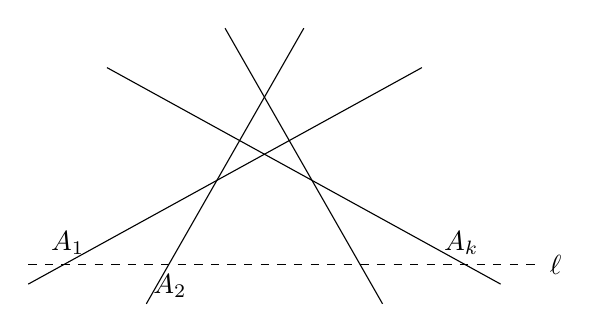
\begin{tikzpicture}%[very thick]
    \draw (1.5,-1)--(-.5,2.5);
    \draw (-1.5,-1)--(.5,2.5);
    \draw (-3,-.75)--(2,2);
    \draw (3,-.75)--(-2,2);
    \node at (-2.5,-.5) [above] {$A_1$};
    \node at (-1.2,-.5) [below] {$A_2$};
    \node at (2.5,-.5) [above] {$A_k$};
    \draw[dashed] (-3,-.5)--(3.5,-.5)node[right]{$\ell $};
  \end{tikzpicture}
  \caption{}\label{fig:lines}
\end{figure}
因为已知任何两条直线不平行,所以直线 $\ell$ 与平面上的原 $k$ 条直线都相交,而且这 $k$ 个交点互不相同,否则与任何三条直线不过同一点的已知条件矛盾,这 $k$ 个交点将直线 $\ell$ 分成 $k+1$ 段,因此直线 $\ell$ 越过原来的 $k+1$ 块平面部分,直线上的每段将它所在的原平面块分成两块,因此要给原来的平面部分的总数 $f(k)$ 增加 $k+1$ 块新的平面部分,就是
\[f(k+1)=f(k)+(k+1)\]
将 $f(k)=\dfrac{1}{2}(k^2+k+2)$ 代入上式,得到
\[\begin{split}
    f(k+1)&=\frac{1}{2}(k^2+k+2)+(k+1)\\
    &=\frac{1}{2}(k^2+3k+4)\\
    &=\frac{1}{2}[(k+1)^2+(k+1)+2]
\end{split}\]
这就是说,当 $n=k+1$ 时,命题也成立。



根据 \ref{itm:proof1_lines} 和 \ref{itm:proof2_lines},可知命题成立。
\end{enumerate}
\end{proof}

同学也许会问:\cref{exp:lines} 的结果是怎样发现的?数学归纳法能解决这个问题吗?其实此题的证明已经解决了这个问题,因为我们证明了 $f(n)$ 可以递归地定义为
\[\begin{cases}
    f(1)=2\\
    f(k+1)=f(k)+(k+1),\qquad k=1,2,\ldots,(n-1)
\end{cases}\]

首先 $f(1)$ 有定义,其次如果知道了 $f(1)$,就知道 $f(2)$,依次推下去,就知道$f(n)$。所以
\[\begin{split}
  f(n)&=[f(n)-f(n-1)]+[f(n-1)-f(n-2)]+\cdots +[f(2)-f(1)]+f(1)\\
  &=n+(n-1)+\cdots +2+2\\
  &=[n+(n-1)+(n-2)+\cdots +2+1]+1\\
  &=\frac{n(n+1)}{2}+1=\frac{n^2+n+2}{2}  
\end{split}\]


\begin{Exercise}
\begin{question}
    \item 用数学归纳法证明下列各等式: 
\begin{tasks}(2)
    \task $\displaystyle\sum^n_{k=1}3^{k-1}=\frac{3^n-1}{2}$
    \task $\displaystyle\sum^n_{k=1}k(k+1)=\frac{1}{3}n(n+1)(n+2)$
    \task $\displaystyle\sum^n_{k=1}\frac{1}{k(k+1)}=\frac{n}{n+1}$
    \task! \[\sum_{i=1}^{n}\cos[\alpha+(i-1)\beta]=\frac{\sin\dfrac{n\beta}{2}}{\sin\dfrac{\beta}{2}}\cos\left(\alpha+\frac{n-1}{2}\beta\right)\]
\end{tasks}

\item 用数学归纳法证明:
\begin{tasks}
\task 当 $n$ 是正整数时,$x^n-y^n$ 能被 $x-y$ 整除。
\task 当 $n$ 是正奇数时,$x^n+y^n$ 能被 $x+y$ 整除。
\task $(3n+1)7^n-1$ 能被 9 整除。
\task 邻近的三个自然数的立方和,必定能被 9 整除。
\task 当 $n$ 是正整数时,$(11)^{n+2}+(12)^{2n+1}$ 能被 133 整除。
\task 当 $n$ 是正整数时,$3^{2n+2}-8n-9$ 能被 64 整除。
\end{tasks}

\item 数列 $\{a_n\}$ 是这样确定的:
\[a1=1,\quad 4a_ka_{k+1}=(a_k+a_{k+1}-1)^2,\quad a_k<a_{k+1}\quad (k=1,2,3,\ldots)\]
\begin{tasks}
  \task\label{tsk:equation} 求 $a_2,a_3,a_4$, 并由此推断 $a_n$;
  \task 用数学归纳法证明 \ref{tsk:equation} 中推断出的 $a_n$ 的正确性。
\end{tasks}

\item 空间有$n$个平面,其中没有两个平面平行,没有三个平面相交于同一条直线,也没有四个平面过同一个点。求证:它们把空间分成 $f(n)=\frac{1}{6}(n^3+5n+6)$ 份。
\item 有 $n$ 个圆,其中每两个圆都相交于两点,并且每三个圆不相交于同一点。求证:这 $n$ 个圆把平面分成 $n^2-n+2$ 部分。
\item 若数列 $\{a_n\}$,当 $n\geqslant 3$ 时,满足条件
\[\frac{1}{a_1a_2}+\frac{1}{a_2a_3}+\frac{1}{a_3a_4}+\cdots+\frac{1}{a_{n-1}a_n}=\frac{n-1}{a_1a_n}\]
用数学归纳法证明数列 $\{a_n\}$ 是等差数列。
\end{question}
\end{Exercise}
\chapter{实数}\label{chp:real}
实数是现实世界中最基本的数系,我们采用逼近法来研究实数,逼近法是一种原理简朴但是应用广泛的方法,它将贯穿于本书的微积分学部分,是一支主力军。

\section{度量与实数}

一般说来,常见的量可以归纳成两类:比如一堆蛋,一群牛,它们都具有天然的个别单元,对它们的处理方法是数一数它们的个数,用来数个数的数学体系就是“自然数系”。另一类量如长度、重量、温度、压力这种量不具有天然不可分割的单元!我们处理这类量的办法是度量,由度量产生的数系就是“实数系”,换句话说,实数系乃是将常见的长度、重量等这一类量的通性加以抽象化、组织化所得出来的数学体系,它是用来表达、计算这一类连续变化的量的简洁、有效工具。

下面将以长度为例,说明度量和实数的起源。

\subsection{长度的度量}
因为长度这种量并不是有天然不可分割的单位,所以我们只好选用人为的单位长,设线段 $u$ 是所选用的单位长,当我们要度量一个线段 $a$ 时,我们所要去求的乃是 $a$ 与 $u$ 之间的“比值”,这个比值是一个实数 $k$, 我们就说线段 $a$ 的长度是 $k$ 单位,现在让我们耐心地分析一下,在实践中这个“比值”是怎样求得的?

我们先拿一根尺 $u$, 用它去逐段比量线段 $a$, 假如 $a$ 恰好是 $n$ 个和 $u$ 等长的线段首尾连接而成,我们说 $u$ 恰好整量 $a$, $a$ 的长度是 $n$ 单位,但是假如 $u$  不能整量 $a$,例如在\cref{fig:segments} 中的线段,$a$ 比 $4u$ 要长些,却比 $5u$ 要短些。

\begin{figure}
\begin{tikzpicture}
\draw (0,1)--node[above]{$u$}(1,1);
\foreach \x in {0,1}
{
    \draw (\x,1)--(\x,1.1);
}
\draw (0,0)--node[above=5pt]{$a$}(4.75,0);
\foreach \x in {0,1,...,4,4.25,4.5,4.75}
{
    \draw (\x,0)--(\x,0.1);
}
\end{tikzpicture}
    \caption{}\label{fig:segments}
\end{figure}

{
\linespread{1.6}\selectfont
试着去解决上述不能整量的矛盾的一个简朴想法是:把单位长 $u$ 适当地加以等分,希望分后的“分单位”能够整量 $a$(比如上面的例子中,$\dfrac{1}{4}u$ 就可以整量 $a$, 即 $a=4\dfrac{3}{4}u=\dfrac{19}{4}u$),一般地,假如 $a$ 能用 $\dfrac{1}{m}u$ 这个分单位整量,譬如 $a=\dfrac{n}{m}u$,则 $a,u$ 之间的比值是个有理数(也称为比数)。在这儿,就自然地产生下述基本问题。\par}

\bigskip
\emph{度量基本问题 } 任给两个量 $a,b$ 之间的比值是否一定是个有理数(比数)?换句话说,对于任给两个量 $a,b$ 是否存在一个同时整量 $a,b$ 的 $u$?

上面这个问题的重要性可以分别从正、反两面来分析:假如任何两个量的比值总是有理数,那么有理数全体就足够处理度量问题,这样度量问题就变得十分简单了。从另一方面来看,假如两个量之间的比值不一定是有理数,则有理数全体(简称有理数系或比数系)就不足以处理度量问题,换句话说,我们就得学会一个不只包含有理数系的实数系,才能充分处理度量问题。总之,上述基本问题是必须实事求是地弄明白的!

\subsection{无理数(非比实数)的存在}
不难给出,两个线段的比值不可能是有理数的一个简单例子,如\cref{fig:irrationalnumber} 所示,各边为单位长度的正方形的对角线 $\ell$ 与边长之比就不能是个有理数。
\begin{figure}
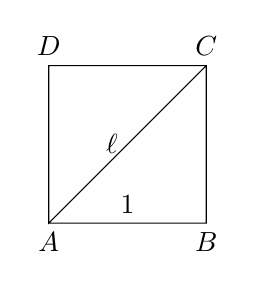
\begin{tikzpicture}
\draw (0,0)node[below]{$A$} --node[above]{1}(2,0)node[below]{$B$}-- (2,2)node[above]{$C$}--(0,2)node[above]{$D$}--(0,0)--node[left]{$\ell$}(2,2);
\end{tikzpicture}
\caption{}\label{fig:irrationalnumber}
\end{figure}

因为根据勾股定理,$\ell^2=2$, 所以,如果 $\ell$ 是个有理数,设其等于 $\dfrac{p}{q}$,这里 $q$ 和 $p$ 是两个互质的正整数,我们将有
\[p^2=2q^2\]
根据上述方程,$p$ 是偶数,因此 $p$ 本身也必定是偶数,譬如说,$p=2p'$, 用 $2p'$ 代替 $p$, 我们得到
\[4({p'}^2)=2q^2\]
或者,
\[q^2=2(p')^2\]
{\linespread{1.6}\selectfont
因而 $q^2$ 是偶数,于是 $q$ 也是偶数,然而这同我们所作的 $p$ 和 $q$ 没有公因子的约定相矛盾,这一矛盾是由假设对角线长能够表示为既约分数 $\dfrac{p}{q}$ 引起的,所以这一假设是错误的。\par}

这一用反证法推导的例子,表明符号 $\sqrt{2}$ 不能对应于任何有理数。另一例子是$\uppi$ ——圆的周长与直径的比,证明 $\uppi$ 不是有理数要复杂得多,并且直到近代才做到。不属于有理数系的实数有很多,所以在某种意义上远比有理数更为普遍,因此,从几何度量的客观实际需要出发,我们不得不增添一类新数,这一类新数叫\emph{无理数}。有理数和无理数的全体统称为\emph{实数系}。当我们面对着实数系中还存在着许多“无理数”这一事实时,怎样去有系统地学习实数系的性质并充分掌握其用法,这便成为我们的一个迫切的基本课题。下面所要谈的逼近法,就是一种有效地利用熟知的有理数系作为桥梁,向实数系进军的捷径。

\subsection{逼近法}
通过已知的有理数系去了解实数系的可能性基于下述基本事实,那就是:任何无理数都可以用有理数去逼近它!现在我们用数轴来图解有理数系与实数系间的关系。如\cref{fig:approximation} 所示。

\begin{figure}
\begin{tikzpicture}[>=latex, scale=1.3]
\draw[very thick, ->] (-0.8,0)--(8,0)node[right]{$\ell$};
\foreach \x/\xtext in {0/0,1/\dfrac{1}{q},2/\dfrac{2}{q},5.5/\dfrac{p}{q},6.5/\dfrac{p+1}{q}}
{
    \draw (\x, 0)node[below]{$\xtext$}--(\x,.1);
} 
\draw (5.9,0)--(5.9,.1)node[above]{$x$};
\end{tikzpicture}
    \caption{}\label{fig:approximation}
\end{figure}

{\linespread{1.6}\selectfont
在上面坐标系中,所有以整数为坐标的点,在直线 $\ell$ 上成一均匀分布的点集,其相邻两点间的距离都是 1 单位;同样的,所有坐标是 $\dfrac{p}{2}$, $(p=0,\pm1,\pm2,\ldots)$ 的点,在直线上成一均匀分布的点集,其相邻两点间的距离都是 $\dfrac{1}{2}$ 单位;设$q$为一指定的自然数,则所有坐标是 $\dfrac{p}{q},\; p\in\mathbb{Z}$ 的点在直线上成一均匀分布的点集,其相邻两点间的距离是 $\dfrac{1}{q}$ 单位。只要将 $q$ 取成足够大的自然数,则能使数 $\dfrac{1}{q}$ 想要多么小就可以多么小。这个现象说明在直线上任何一段很短的线段中,都有坐标是有理数的点,也就是任何两个有理数点之间都有有理数点,这就是\emph{有理数点集稠密性},但是这个现象并不表示有理点就可以填满整个直线,例如长度为 $\sqrt{2}$, $\sqrt{3}$ 的线段,若将它的一个端点放在数轴的原点,则另一端点在直线的坐标就不是有理数。现在我们的问题是如何说明实数同原来熟悉的有理数,因而最终同整数的关系。让我们再回到\cref{fig:approximation} 的数轴 $\ell$上,显然 $\ell$ 上面的每一个点或者是坐标为 $\dfrac{p}{q}$ 的有理点,或者处于两个相邻的有理点 $\dfrac{p}{q}$和$\dfrac{p+1}{q}$ 之间,换言之,给了任何自然数 $q$ 之后,对于每一个实数 $x$, 一定有一整数  $p$, 使得\par}
\[\frac{p}{q}\leqslant x<\frac{p+1}{q}\]
即
\[\frac{p}{q}\leqslant x<\frac{p}{q}+\frac{1}{q}\]
从这三个数各减去 $\dfrac{p}{q}$,得到
\[0\leqslant x-\frac{p}{q}<\frac{1}{q}\]
于是
\[\left|x-\frac{p}{q}\right|<\frac{1}{q}\]
这个不等式说明,只要将 $q$ 取成足够大的自然数,每一个实数 $x$ 与有理数 $\dfrac{p}{q}$ 的误差想要多么小就可以多么小。

下面我们来说明每一个无理数如何通过越来越逼近它的有理数数列来描述它。

\subsubsection{二分逼近法}

现在让我们用二分逼近法来说明任何无理数都可以用有理数数列去逼近它,使得误差小到任意小。

设某无理数 $x$ 位于线段 $A_0B_0=[a_0,b_0]$ 内(亦即$a_0<x<b_0$,$a_0$,$b_0$ 均为有理数),见\cref{fig:rationalnumber}。

\begin{figure}
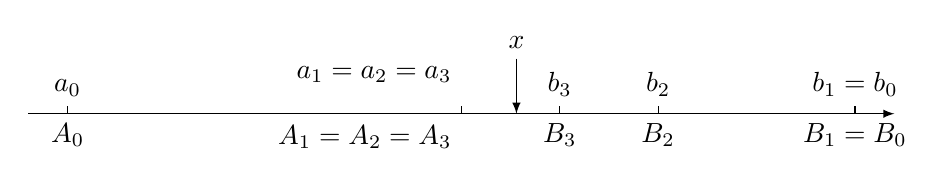
\begin{tikzpicture}[>=latex]
\draw[->] (-0.5,0)--(10.5,0);
\foreach \x/\xtext in {0/a_0,10/b_1=b_0,7.5/b_2,6.25/b_3}
{
    \draw (\x,0)--(\x,.1)node[above]{$\xtext$};
}  
\draw (5,0)--(5,.1);

\node at  (5,-.3)[left]{$A_1=A_2=A_3$};
\node at (6.25,0)[below]{$B_3$};
\node at (7.5,0)[below]{$B_2$};
\node at (0,0)[below]{$A_0$};
\node at (10,0)[below]{$B_1=B_0$};
\node at  (5,.5)[left]{$a_1=a_2=a_3$};
\draw[->] (5.7,.7)node[above]{$x$}--(5.7,0);
\end{tikzpicture}   
    \caption{}\label{fig:rationalnumber}
\end{figure}

{\linespread{1.6}\selectfont 我们将线段 $A_0B_0=[a_0,b_0]$ 等分为两段,亦即 $\left[a_0,\dfrac{a_0+b_0}{2}\right]$ 和 $\left[\dfrac{a_0+b_0}{2},b_0\right]$;而把 $x$ 所在的那一段叫做 $A_1B_1=[a_1,b_1]$,换句话说,当 $a_0<x<\dfrac{a_0+b_0}{2}$ 时,$a_1=a_0$,$b_1=\frac{a_0+b_0}{2}$;当 $\dfrac{a_0+b_0}{2}<x<b_0$,$a_1=\dfrac{a_0+b_0}{2}$,$b_1=b_0$。这样逐次二等分,由 $A_1B_1$ 求得 $A_2B_2$,\ldots,由 $A_{n-1}B_{n-1}$ 求得 $A_nB_n$,永远无休止地二等分下去,因为每次二等分后,分段长度减半,所以 $x$ 所在的线段就可以小到任何需要的程度。现在把上面的二分逼近过程写下来,就得到 $a_n,b_n,x$ 的下列关系:\par}
\begin{enumerate}
    \item $A_0B_0=[a_0, b_0]\supseteq A_1B_1 =[a_1,b_1]
    \supseteq \cdots \supseteq A_nB_n=[a_n, b_n]\supseteq A_{n+1}B_{n+1}=[a_{n+1},b_{n+1}]\supseteq \cdots \supseteq \{x\}$,即:
\[a_0\leqslant a_1\leqslant a_2\le\cdots\leqslant a_n\leqslant \cdots <x<\cdots\leqslant b_n\le\cdots\leqslant b_2\leqslant b_1\leqslant b_0\]

\item {\linespread{1.6}\selectfont $b_n-a_n=\dfrac{1}{2}(b_{n-1}-a_{n-1})=\cdots=\dfrac{1}{2^n}(b_0-a_0)$,这就保证了 $a_n$ 或 $b_n$ 和 $x$ 之间的误差小于 $\dfrac{1}{2^n}(b_0-a_0)$, 即 $|x-a_n|<\dfrac{1}{2^n}(b_0-a_0)$ 或 $|x-b_n|<\dfrac{1}{2^n}(b_0-a_0)$, 只要 $n$ 够大,上述误差就可以小到任意小。\par}
\item 实数 $x$ 由它的夹逼数列:
\[a_0\leqslant a_1\leqslant a_2\le\cdots\leqslant a_n\leqslant \cdots <x<\cdots\leqslant b_n\le\cdots\leqslant b_2\leqslant b_1\leqslant b_0\]
其中:$b_n-a_n=\dfrac{1}{2^n}(b_0-a_0)$ 唯一确定,即没有另一点能够处在所有的线段 $A_nB_n$ 之中。
\end{enumerate}

要证明这个数的唯一性,我们假定另有第二个数 $y$ 也属于一切线段 $A_nB_n$ 之中,于是这些线段的每一个长 $b_n-a_n$ 都应不小于 $|x-y|$, 但是,因为线段 $A_nB_n$ 可以任意小,只要 $n$ 足够大,$A_nB_n$ 的长就会小于 $x$ 和 $y$ 之间的距离,这就得出矛盾。所以实数 $x$ 能由它的夹逼数列唯一确定。

现在以 $x=\sqrt{2}$, $a_0=1$, $b_0=2$ 为例来说明如何用二分逼近法求 $\sqrt{2}$ 的近似值,如\cref{fig:sqrt2} 所示。
\begin{figure}
\begin{tikzpicture}[>=latex]
    \draw[->] (-0.5,0)--(10.5,0);
\foreach \x /\xtext in {0/a_0=a_1=1,10/b_0=2,5/{},2.5/a_2,3.75/a_3=a_4, 4.375/{}}
{
    \draw(\x,0)--(\x,.1)node[above]{$\xtext$};
}

\draw[->] (4.14,-.7)node[below]{$\sqrt{2}$}--(4.14,0);

\node at (5,-0.3)[right]{$b_1=b_2=b_3$};
\node at (4.375,-0.3){$b_4$};
\end{tikzpicture}
    \caption{}\label{fig:sqrt2}
\end{figure}

\begin{enumerate}
    \item  $\dfrac{1}{2}\left(a_{0}+b_{0}\right)=\dfrac{3}{2},\qquad \left(-\dfrac{3}{2}\right)^{2}=\dfrac{9}{4}>2 \quad\Rightarrow\quad\dfrac{3}{2}>\sqrt{2}$,
    
    故 $a_{0}=a_{1}=1,\qquad   b_{1}=\dfrac{3}{2}$

    \item   $\dfrac{1}{2}\left(a_{1}+b_{1}\right)=\dfrac{5}{4},\qquad \left(\dfrac{5}{4}\right)^{2}=\dfrac{25}{16}<2 \quad\Rightarrow\quad \dfrac{5}{4}<\sqrt{2}$
    
    故 $a_{2}=\dfrac{5}{4}, \qquad  b_{2}=b_{1}=\dfrac{3}{2}$

    \item  $\dfrac{1}{2}\left(a_{2}+b_{2}\right)=\dfrac{11}{8},\qquad \left(\dfrac{11}{8}\right)^{2}=\dfrac{121}{64}<2 \quad\Rightarrow\quad \dfrac{11}{8}<\sqrt{2}$
    
    故 $a_{3}=\dfrac{11}{8},\qquad  b_{3}=b_{2}=\dfrac{3}{2}$

    \item   $\dfrac{1}{2}\left(a_{3}+b_{3}\right)=\dfrac{23}{16},\qquad \left(\dfrac{23}{16}\right)^{2}=\dfrac{529}{256}>2 \quad\Rightarrow\quad \dfrac{23}{16}>\sqrt{2}$
    
    故 $a_{4}=a_{3}=\dfrac{11}{8},\qquad  b_{4}=\dfrac{23}{16}$

    \item  $\dfrac{1}{2}\left(a_{4}+b_{4}\right)=\dfrac{45}{32},\quad \left(\dfrac{45}{32}\right)^{2}=\dfrac{2025}{1024}<2 \quad\Rightarrow\quad \dfrac{45}{32}<\sqrt{2}$
    
     故 $a_{5}=\dfrac{45}{32}, \qquad b_{5}=b_{4}=\dfrac{23}{16}
    $
    
    \item  $\dfrac{1}{2}\left(a_{5}+b_{5}\right)=\dfrac{91}{64},\quad \left(\dfrac{91}{64}\right)^{2}=\dfrac{8281}{4096}>2 \quad\Rightarrow\quad \dfrac{91}{64}>\sqrt{2}$
    
     故 $a_{6}=a_{5}=\dfrac{45}{32}, \qquad b_{6}=\dfrac{91}{64}$

    
    \item  $\dfrac{1}{2}\left(a_{6}+b_{6}\right)=\dfrac{181}{128},\quad \left(\dfrac{181}{128}\right)^{2}=\dfrac{32761}{16314}<2 \quad\Rightarrow\quad \dfrac{181}{128}<\sqrt{2}$
    
    {\linespread{1.9}\selectfont 故 $a_{7}=\dfrac{181}{128}, \qquad b_{7}=b_{6}=\dfrac{91}{64}$,这时,$\dfrac{181}{128}<\sqrt{2}<\dfrac{91}{64}$,把 $\dfrac{181}{128}$ 作为 $\sqrt{2}$ 的不足近似值,其误差小于 $\dfrac{1}{2^7}=\dfrac{1}{128}$。\par}
\end{enumerate}

\medskip
{\linespread{1.6}\selectfont 照这样逐步计算,每次只要检验 $\dfrac{1}{2}(a_{n-1}+b_{n-1})$ 的平方和 2 之间的大小次序关系,就能确定 $\dfrac{1}{2}(a_{n-1}+b_{n-1})$ 应该是 $a_n$ 还是 $b_n$, 显然的,这样所求得的 $a_n,b_n$ 和 $\sqrt{2}$ 有下列关系:\par}
\[a_n<\sqrt{2}<b_n,\quad b_n-a_n=\frac{1}{2^n},\; (n=1,2,3,\ldots)\]

我们可以把 $a_n$ 叫做 $\sqrt{2}$ 的一个“$n$ 阶不足近似值”。$b_n$ 叫做 $\sqrt{2}$ 的一个“$n$ 阶过剩近似值”,它们和 $\sqrt{2}$ 的差的绝对值小于 $\dfrac{1}{2^n}$。


\subsubsection{十分逼近法}

上面所讨论的二分逼近法只不过是逼近法的一种,譬如,对于任何大于 1 的整数 $q$, 我们可以仿照上法用逐次 $q$ 等分而得到“ $q$ 分逼近法”,但是实用起来,$q$ 愈大则每次要去确定 $x$ 属于 $q$ 个分段中的哪一段时所需做计算也就愈繁,所以二分逼近法比较简便,再者,在 $q$ 分逼近法中,用来逼近的数 $a_n,b_n$ 都是那些分母是 $q$ 的方幂的分数;而常用的“十进小数”也就是分母是 10 的方幂的分数,例如,
\[1.4=\frac{14}{10},\quad  1.41=\frac{141}{100}=\frac{141}{10^2},\quad \ldots \]
所以十分逼近法也就是用小数去逼近的方法,现在再以 $\sqrt{2}$ 为例,简要地说明十分逼近法如下:

将线段 $[1,2]$ 十等分,其分点分别是 $1.1,1.2,\ldots,1.9$, 看看哪些分点的平方小于 2, 哪些大于 2,算一下就得出:

$(1.1)^2,(1.2)^2,(1.3)^2,(1.4)^2=1.96<2<2.25=(1.5)^2,(1.6)^2,\ldots ,(1.9)^2$。所以 $1.4<\sqrt{2}<1.5$,$\sqrt{2}$ 属于分段 $[1.4,1.5]$;

再把 $[1.4,1.5]$ 十等分,分点分别是 $1.41,1.42,\ldots,1.49$,再算一下,由$(1.41)^2=1.9891<2<2.0164=(1.42)^2,(1.43)^2,\ldots,(1.49)^2$,就得出 $\sqrt{2}$ 属于分段 $[1.41,1.42]$,再一次十等分,然后再由计算可以确定 $\sqrt{2}$ 属于分段  $[1.414,1.415]$,这样逐次十等分,就可以求得一个 $n$ 位小数 $a_n$ 使得
\[a_n<\sqrt{2}<b_n=a_n+\left(\frac{1}{10}\right)^n\]

在实用时,我们按照实际问题所需要的精确度,求到足够位数(即 $\left(\frac{1}{10}\right)^n$ 小于许可误差)。这里我们用普通的算术法则对 2 作开方运算将得到一个足够精确的小数。例如,求 $\sqrt{2}$ 的不足近似值和过剩近似值,精确到 $\dfrac{1}{10^4}$。计算如下:

\begin{center}
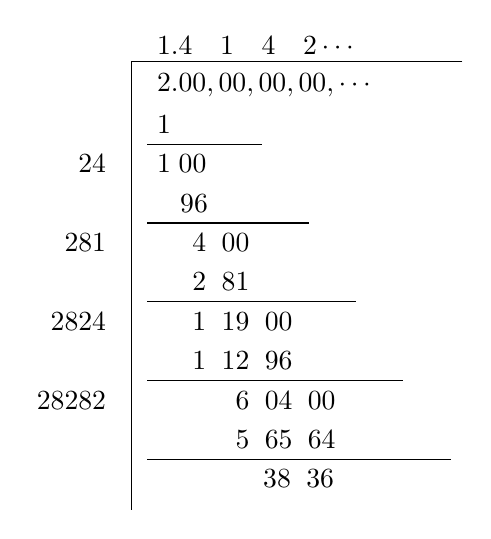
\begin{tikzpicture}[scale=2]
\node at (0,0)[right]{$\qquad \quad\;\;\;  38\;\;36$};
\node at (0,0.25)[right]{$\qquad\;\;\;  5\;\;65\;\;64$};
\node at (0,0.5)[right]{$\qquad \;\;\; 6\;\;04\;\;00$};
\node at (0,0.75)[right]{$\quad \; 1\;\;12\;\;96$};
\node at (0,1)[right]{$\quad \; 1\;\;19\;\;00$};
\node at (0,1.25)[right]{$\quad\; 2\;\;81$};
\node at (0,1.5)[right]{$\quad \; 4\;\;00$};
\node at (0,1.75)[right]{$\;\;\; 96$};
\node at (0,2)[right]{$1\;00$};
\node at (0,2.25)[right]{$1$};
\node at (0,2.5)[right]{$2.00,00,00,00,\cdots$};
\node at (0,2.75)[right]{$1.4\quad1\quad4\quad2\cdots$};
\draw(2,2.65)--(-0.1,2.65)--(-0.1,-.2);

\foreach \x/\xtext in {2/24,1.5/281,1/2824,.5/28282}
{
   \node at (-.2,\x)[left]{\xtext};
}

\foreach \x in {2.125,1.625,...,0.125}
{
    \draw (0,\x)--(2-.6*\x,\x);
}
\end{tikzpicture}
\end{center}

从计算中知道
\[1.4142<\sqrt{2}<1.4143\]
\[|\sqrt{2}-1.4142|<\frac{1}{10^4}, \qquad |\sqrt{2}-1.4143|<\frac{1}{10^4}\]

因此,1.4142, 1.4143 分别是 $\sqrt{2}$ 的精确到 $\dfrac{1}{10^4}$ 的不足近似值与过剩近似值。

\medskip
总结上面对于逼近法的讨论,我们得到了下列几点简要的初步认识:
\begin{enumerate}
    \item 实数系,有理数系,整数系,自然数系的包含关系是这样的:
\[\begin{split}
    &\qquad \mathbb{R}\quad \supset \quad \mathbb{Q}\quad \supset \quad \mathbb{Z}\quad \supset \quad \mathbb{N}\\
    &\text{实数系\quad 有理数系\quad 整数系\quad 自然数系}
\end{split}
\]

实数系还包括无理数,任何无理数都可以用有理数去逼近它!二分逼近法和 $q$ 分逼近法是各种逼近法中最常用的几种。
\item 一般说来,逼近法就是对于某一给定实数 $x$ 逐步地去求它的近似值 $a_n$,使得误差 $|x-a_n|$ 可以小到任意小。在 $q$ 分法中,使得误差小到任意小的办法是用逐次$q$ 等分同时求出一个“不足近似值” $a_n$ 和一个“过剩近似值” $b_n$,它们把所要逼近的实数 $x$ 夹逼在当中,即 $a_n<x<b_n$。因为当 $n$ 逐步增大时,$b_n-a_n=\dfrac{b_0-a_0}{q^n}$ 是显然可以小到任意小!这也就是说,给定实数 $x$ 由它的不足近似值数列 $\{a_1,a_2,\ldots ,a_n,\ldots\}$ 和过剩近似值数列 $\{b_1,b_2,b_3,\ldots ,b_n,\ldots \}$ 唯一确定。

\item 更普遍地,对给定的实数 $x$, 用某种方法得到两
个无穷数列 $\{a_1,a_2,\ldots ,a_n,\ldots\}$ 和 $\{b_1,b_2,\ldots ,b_n,\ldots \}$, 它们和 $x$ 之间满足下列关系:
\[a_1\leqslant a_2\leqslant \cdots \leqslant a_n\leqslant \cdots<x<\cdots\leqslant b_n\leqslant \cdots\leqslant b_2\leqslant b_1\]
而且在 $n$ 不断增大时,$(b_n-a_n)$ 可以小到任意小,则 $\{a_n\}$ 就叫做 $x$ 的一个“左逼近数列”,$\{b_n\}$ 就叫做 $x$ 的一个“右逼近数列”,它们分别从左、右夹逼 $x$,这样,$x$ 也就由这两组数列唯一确定。
\end{enumerate}


\subsection{实数系的基本性质}
实数系是计算长度、面积、重量、时间等等这一类量不可缺少的工具。实数系具有四则运和大小次序这两种基本结构。现在我们先以线段的长度为例,从几何上定义实数系的四则运算和大小次序,这样,同学就容易从几何上验证实数(线段长度)满足有理数系的四则运算和大小次序的基本性质。然后,我们将在第七章利用数列极限的概念再给出实数的算术运算的定义。

将两个线段 $AB$, $CD $互相叠置,使 $A$ 点与 $C$ 点重合,如果 $D$ 点不与 $B$ 点重合,落在线段 $AB$ 上,那么线段 $AB$ 的长度 $k$ 个单位就大于线段 $CD$ 的长度 $\ell$ 个单位,记作 $k>\ell$;如果 $D$ 点落在线段 $AB$ 的延长线上,那么线段 $AB$ 的长度就小于线段 $CD$ 的长度,记作$k<\ell$;如果 $D$ 点与 $B$ 点重合则说线段 $AB$ 与 $CD$ 有相等长度,记作$k=\ell$。

我们定义,和 $k+\ell$ 与差 $k-\ell\; (k>\ell )$ 分别是线段的几何和与差的长度。

例如线段 $AB$ 的长度是 $k$ 单位,$BC$ 的长度是 $\ell$ 单位,则线段 $AC$ 的长度就是 $(k+\ell)$ 单位,如\cref{fig:length} 所示。
\begin{figure}
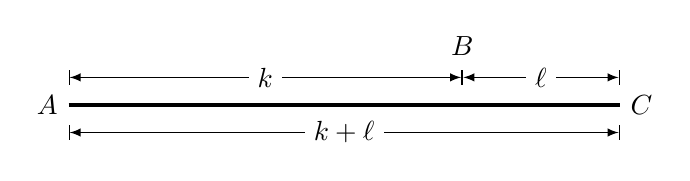
\begin{tikzpicture}[>=latex]
\draw[|<->|] (0,-.35)--node[fill=white]{$k+\ell$}(7,-.35);
\draw[|<->|] (0,.35)--node[fill=white]{$k$}(5,.35);
\draw[|<->|] (5,.35)--node[fill=white]{$\ell$}(7,.35);
\node at (5,.5)[above]{$B$};
\draw[very thick](0,0)node[left]{$A$}--(7,0)node[right]{$C$};

\end{tikzpicture}
    \caption{}\label{fig:length}
\end{figure}

现在我们定义积 $ab$,如\cref{fig:production1},画了一个任意角,在它的一边上,从顶点开始顺次截取长度为 1 和 $b$ 的线段 $OA$ 和 $AC$,在另一边上截取长度为 $a$ 的线段 $OB$,此外,作直线 $CD$ 平行于直线 $AB$,$CD$ 截得的线段 $BD$ 的长度,定义为积 $ab$。这个定义是合理的,因为如果我们在另一个角 $O'$ 上类似地作图(\cref{fig:production2}),那么得到的线段 $B'D'$ 的长度和线段 $BD$ 的长度相等。

\begin{figure}
\begin{minipage}{0.48\linewidth}
  \centering
  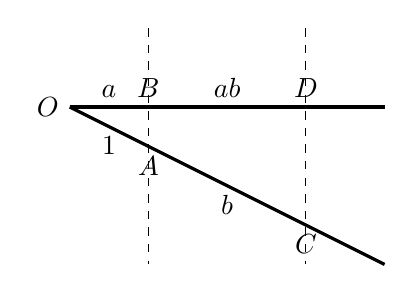
\begin{tikzpicture}
    \draw[very thick] (0,0)node[left]{$O$}--(4,0);
    \draw[very thick] (0,0)--(4,-2);
    \draw[dashed] (1,1)--(1,-2);
    \draw[dashed]  (3,1)--(3,-2);
    \foreach \x/\xtext in {1/B,3/D}
    {
        \node at (\x,0) [above]{$\xtext$};
    }
    \foreach \x/\xtext in {1/A,3/C}
    {
        \node at (\x,-.5*\x) [below]{$\xtext$};
    }
% \node at (2,-2.5){$(1)$};
    \node at (.5,-.25)[below]{1};
    \node at (.5,0)[above]{$a$};
    \node at (2,-1)[below]{$b$};
    \node at (2,0)[above]{$ab$};
  \end{tikzpicture}
  \subcaption{}\label{fig:production1}
\end{minipage}
\begin{minipage}{0.48\linewidth}
  \centering
  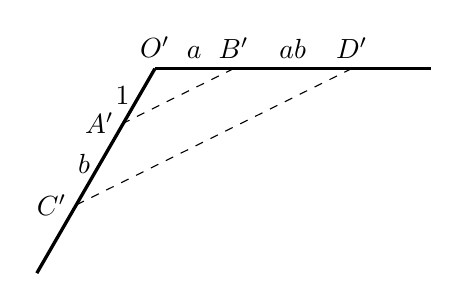
\begin{tikzpicture}
    \draw[very thick] (0,0)node[above]{$O'$}--(3.5,0);
    \draw[very thick] (0,0)--(-120:3);
    \draw[dashed]  (1,0)node[above]{$B'$}--(-120:.8)node[left]{$A'$};
    \draw[dashed]  (2.5,0)node[above]{$D'$}--(-120:2)node[left]{$C'$};
    \node at (.5,0)[above]{$a$};
    \node at (-120:1.4)[left]{$b$};
    \node at (3.5/2,0)[above]{$ab$};
    \node at (-120:.4)[left]{$1$};
  \end{tikzpicture}
  \subcaption{}\label{fig:production2}
\end{minipage}
    \caption{}
\end{figure}

除法运算定义为乘法的逆运算。如\cref{fig:division}, 在角的一边上从顶点开始,顺次截取长度为 $b$ 和 $a$ 的线段,而在另一边上截取单位线段,作 $CD$ 平行于 $AB$, 于是 $AC$ 的长度定义为 $\dfrac{a}{b}$ 这个定义也是合理的,并且 $b\left(\dfrac{a}{b}\right)=a$。

\medskip
最后,我们来规定负长度和零长度。在数轴上,原点 $O$ 右边的点和这点与点 $O$ 的连接线段的长度成一一对应,我们把这种长度称为正的长度。我们把直线上关于原点 $O$ 和点$A$ (即对应长度为 $a$ 的点)对称的点 $A'$ 的相应线段的长度,形式地规定为负的长度 $-a$, 规定点 $O$ 对应于长度零。结果在整个直线上的点和实数之间建立了一一对应。

现在从几何上容易验证实数在四则运算和大小次序这两种结构上满足下面的基本性质,例如,用\cref{fig:distributive_law} 可以验证分配律 $a(b+c)=ab+ac$。

\begin{figure}[htp]
    \begin{minipage}[t]{0.48\textwidth}
    \centering
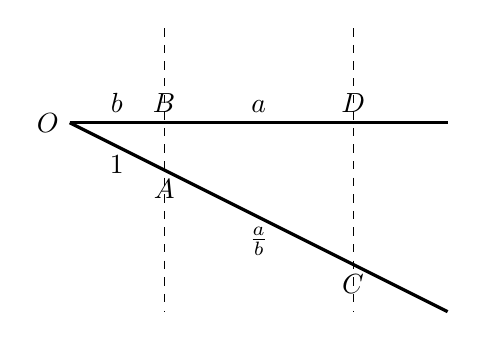
\begin{tikzpicture}[>=latex, scale=1.2]
    \draw[very thick] (0,0)node[left]{$O$}--(4,0);
    \draw[very thick] (0,0)--(4,-2);
    \draw[dashed] (1,1)--(1,-2);
    \draw[dashed]  (3,1)--(3,-2);
    \foreach \x/\xtext in {1/B,3/D}
    {
        \node at (\x,0) [above]{$\xtext$};
    }
    \foreach \x/\xtext in {1/A,3/C}
    {
        \node at (\x,-.5*\x) [below]{$\xtext$};
    }

\node at (.5,-.25)[below]{1};
\node at (.5,0)[above]{$b$};
\node at (2,-1)[below]{$\frac{a}{b}$};
\node at (2,0)[above]{$a$};   
    \end{tikzpicture}
    \caption{}\label{fig:division}
    \end{minipage}
    \begin{minipage}[t]{0.48\textwidth}
    \centering
    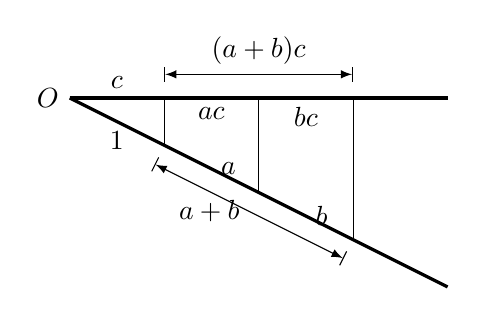
\begin{tikzpicture}[>=latex, scale=1.2]
 \draw[very thick] (0,0)node[left]{$O$}--(4,0);
    \draw[very thick] (0,0)--(4,-2);
    \draw (1,0)--(1,-.5);
    \draw  (2,0)--(2,-1);
    \draw  (3,0)--(3,-1.5);
\node at (.5,-.25)[below]{1};
\node at (.5,0)[above]{$c$};
\node at (1.5,0)[below]{$ac$};   
\node at (2.5,0)[below]{$bc$};   
\node at (1.5,-0.75)[right]{$a$};   
\node at (2.5,-1.25)[right]{$b$};  
\draw[|<->|] (1,.25)--node[above]{$(a+b)c$}(3,.25);
\draw[|<->|] (1-.1,-.5-.2)--node[left]{$a+b$}(3-.1,-1.5-.2);
    \end{tikzpicture}
    \caption{}\label{fig:distributive_law}
    \end{minipage}
    \end{figure}

\subsubsection{加法和乘法的运算性质}

\begin{enumerate}
  \item 交换律:$a+b=b+a;\qquad  ab=ba$
  \item 结合律:$(a+b)+c=a+(b+c);\qquad (a\cdot b)\cdot c=a\cdot (b\cdot c)$
  \item 分配律:$a\cdot (b+c)=a\cdot b+a\cdot c$
  \item 可逆性:$a+x=b;\qquad a\cdot x=b\; (a\ne 0)$ 都是唯一可解的,第一式的解是 $b-a$;第二式的解是 $b/a$。
\end{enumerate}

\subsubsection{顺序性}
\begin{enumerate}
  \item 对于任意实数 $a,b$, 下列关系中有一种且仅有一种成立:
  \[a>b,\qquad a=b\quad \text{或}\quad a<b\]
  \item 由$a<b$和$b<c$推出$a<c$(符号“$<$”的传递性)。
  \item 设$a<b$则$a+c<b+c$
  \item 符号定则
  \[\begin{cases}
      a>0,\qquad b>0\\
      a>0,\qquad b<0\\
      a<0,\qquad b<0
  \end{cases}\Rightarrow\quad  \begin{cases}
      a\cdot b>0\\a\cdot b<0\\a\cdot b>0\\
  \end{cases}\]
  \item 对于任意两个正实数,$a,b>0$, 恒存有一够大的正整数 $n$, 使得 $na<b$。 (通常称之为阿基米德性质)
\end{enumerate}

\subsubsection{ 实数集连续性(完备性)}
我们已经知道实数系与有理数系在加、乘及不等式的运算上有完全相同的性质,但是实数系还具有一个有理数系所没有的优良性质,那就是下面讨论的实数系连续性(完备性)。

在前面,我们用二分法和十分法为例,说明了任何给定的实数 $x$ 都可以用有理数去逼近它。我们所用的是两个有理数列 $\{a_n\}$ 和 $\{b_n\}$ 从左、右夹逼 $x$,$\{a_n\}$,$\{b_n\}$ 和 $x$ 之间的关系可以用下面这一串次序关系来表达:
\[a_1\leqslant a_2\le\cdots\leqslant a_n\leqslant \cdots <x<\cdots\leqslant b_n\leqslant \cdots\leqslant b_2\leqslant b_1\]
$(b_n-a_n)$ 可以任意小,记作 $(b_n-a_n)\to 0$。上面是实数 $x$ 已经先给定了的情况,去求出两串数列 $\{a_n\}$ 和 $\{b_n\}$ 来左、右夹逼实数 $x$,也就是说,数轴$\ell$ 上的每一点,即每一个实数,能够由上述的两个有理数列来唯一确定。反过来问,假如先给定了满足下述这样一串大小次序关系的 $\{a_n\}$ 和 $\{b_n\}$,即
\[a_1\leqslant a_2\le\cdots\leqslant a_n\leqslant \cdots \leqslant b_n\leqslant \cdots\leqslant b_2\leqslant b_1\]
且 $(b_n-a_n)$ 可以任意小,是不是会有那么一个实数 $x$ 去被 $\{a_n\}$、$\{b_n\}$ 左、右夹逼呢?上述问题的答案是肯定的!因为从实数系在长度度量的直观上看,这个实数$x$ 的存在也就是说实数轴上没有空隙存在,即直线是连续不断的,换言之,实数系也是连续不断的,因此我们称实数系为\emph{实数连续统};它说明实数系包含着度量时所有应该包含的数,所以也叫做实数系的\emph{完备性}。下面是直线连续不断的直观概念的解析
描述。

\begin{Theorem}[实数系完备性]{性质}
  对于任给满足下述大小次序关系的两个数列 $\{a_n\}$ 和 $\{b_n\}$,即
\[a_1\leqslant a_2\leqslant \cdots a_n\leqslant \cdots \leqslant b_n\leqslant \cdots \leqslant b_2\leqslant b_1\]
且 $(b_n-a_n)\to 0$,则必定存在一个介于所有 $a_n,b_n$ 之间的实数 $x$。
\end{Theorem}

实数系的完备性是非常基本而且重要的!在以后的章节中,我们将用这个性质来证明极限的存在,从而可进行一切极限运算,而这些运算乃是微积分的基础。在每次用到时,我们将详细解说其用法。这样逐步渐近,同学不难学会它的种种用法。

\begin{Exercise}
\begin{question}
  \item 证明 $\sqrt{3}$ 是无理数。
  \item 设 $\sqrt{5}=a$,$a$ 的小数部分用 $b$ 表示,求 $a-\dfrac{1}{b}$。
  \item 若 $a+\sqrt{b}=c+\sqrt{d}$, 这里 $a,b,c,d$ 是有理数而 $\sqrt{b}$ 是无理数,则 $a=c$,$b=d$,试证之。
  \item 利用“整系数方程 $a_0x^n+a_1x^{n-1}+\cdots+a_{n-1}x+a_n=0$ 的任何有理根,如果写成既约分数时为 $\dfrac{p}{q}$,那么分子 $p$ 是 $a_n$ 的约数,分母 $q$ 是 $a_0$ 的约数”,这一准则使我们能够得到一切有理实根,从而证明任何其它根都是无理数。试证明:$3+2\sqrt{2}$,$1+\sqrt[3]{3}$,$\sqrt[3]{2}+\sqrt[3]{4}$ 都是某一整系数方程的无理根,从而证明这些数都是无理数。
  \item 
  \begin{tasks}
    \task 如果 $a$ 是有理数,$x$ 是无理数,试证明 $a+x$ 是无理数;又如果 $a \neq 0$, 试证明 $ax$ 是无理数。
    \task 试证明任何两个有理数之间至少存在着一个无理数,因而存在着无穷多个无理数。
  \end{tasks}
  \item 试证明:任给无理数 $a$ 和正整数 $m$, 我们可以找到分数 $\dfrac{n}{m}$,使得 \[\left|a-\frac{n}{m}\right|<\frac{1}{2m}\]
  \item 若等腰三角形的顶角为 \ang{36},底边长为 1, 试证它的腰长不能用有理数表示。
  \item 用二分逼近法求下列无理数的有理近似值,使得误差小于 $1/100$:
    \begin{tasks}(2)
        \task $\sqrt{7}$
        \task $\sqrt[3]{2}$
    \end{tasks}
\end{question}
\end{Exercise}

\section{不等式与绝对值}
不等式在高等数学中所起的作用要比在初等数学中大得多,一个量 $x$ 的精确值往往难以确定,不过,对 $x$ 进行估值,即指明 $x$ 大于某个已知量 $a$ 而小于另一个已知量 $b$,却是容易做到的。在许多应用中,重要的只是知道 $x$ 的这种估值。为以后学习方便起见,我们要在这一节比较详细地回顾一下不等式的一些重要性质。

\subsection{不等式的性质}
$a$ 和 $b$ 是实数,如果 $a-b>0$,那么就称 $a$ 大于 $b$,记作 $a>b$;如果 $a-b<0$,那么就称 $a$ 小于 $b$,记作 $a<b$;如果 $a-b=0$ 那么就称 $a$ 等于 $b$,记作 $a=b$。注意若 $a<b$ 有时也说成 $b>a$,因此 $a<b$ 和 $b>a$ 是等价的。

应用两个正实数之和或积仍然是正数这个基本事实,即如果 $a>0$ 和 $b>0$ 则有$a+b>0$ 和 $ab>0$,而且依据不等式 $a>b$ 等价于 $a-b>0$,我们容易推导出下面的性质。

\begin{Theorem}{性质1}
  若 $a>b$ 和 $c>d$,则 $a+c>b+d$。换言之,同向的两个不等式可以相加。
\end{Theorem}

\begin{Theorem}{性质2}
  若 $a>b$ 且 $c>0$,则 $ac>bc$。
\end{Theorem}

\begin{Theorem}{性质3}
  若 $a>b$ 且 $c<0$, 则 $ac<bc$。
\end{Theorem}

上面的性质 2 和性质 3 也可以表达为不等式若乘以正数得到同向不等式;若乘以负数则得到异向的不等式。更一般地可以得到:

若 $a>b>0$ 和 $c>d>0$ 则 $ac>bd$。也就是两个同向的正数不等式可以相乘。
\begin{Theorem}{性质4}
  \begin{itemize}
    \item 若 $a>b>0$, 则 $1/a<  1/b$;
    \item 若 $a>0>b$, 则 $1/a>0>1/b$;
    \item 若 $a<b<0$, 则 $1/a>  1/b$。
  \end{itemize}
\end{Theorem}   

\begin{Theorem}{性质5}
  若 $a>b$ 而 $b>c$, 则 $a>c$。
\end{Theorem}

这就是说不等式具有传递性,在几何上这是显然的,也可由 $(a-b)+(b-c)=a-c$ 为正直接推出,在上述推演中,如果我们处处都用符号 $\geqslant $ 代替 $>$,则各项法则仍然成立。

\begin{Theorem}{性质6}
  若 $a>b>0$, 则 $a^2>b^2$。
\end{Theorem}

我们注意到 $a^2-b^2=(a+b)(a-b)$, 因为 $a+b$ 是正数,由 $a>b$ 可以推出,$a^2>b^2$。这样正数之间不等式可以进行平方运算。

\begin{Theorem}{性质7}
  若 $a>b>0$, 则 $\sqrt{a}>\sqrt{b}$,即在正实数之间的不等式两端能取平方根。
\end{Theorem}

事实上,$\sqrt{a}-\sqrt{b}=\dfrac{a-b}{\sqrt{a}+\sqrt{b}}$,因为 $\sqrt{a}+\sqrt{b}$ 是正数,从而由 $a>b$ 就可推出 $\sqrt{a}-\sqrt{b}>0$, 即$\sqrt{a}>\sqrt{b}$。

更一般地,若 $a>b>0$ 且 $n$ 是自然数,那么 $a^n>b^n$。

这个结论可以用数学归纳法来证明。这个证明留给同学作为练习。

\medskip
反过来,若 $a>b>0$, 且 $n$ 是一个正整数,则 $a^{\frac{1}{n}}>b^{\frac{1}{n}}$。

\begin{proof}
\linespread{1.5}\selectfont
假设 $a^{\frac{1}{n}}=b^{\frac{1}{n}}$,那么$\Big(a^{\tfrac{1}{n}}\Big)^n>\Big(b^{\tfrac{1}{n}}\Big)^n$,因而,$a=b$,这就与已知 $a>b$ 矛盾。

假设 $a^{\frac{1}{n}}<b^{\frac{1}{n}}$,于是 $\Big(a^{\tfrac{1}{n}}\Big)^n<\Big(b^{\tfrac{1}{n}}\Big)^n$,即 $a<b$,这又与已知条件 $a>b>0$ 矛盾,故我们得出结论 $a^{\tfrac{1}{n}}>b^{\tfrac{1}{n}}$。\par
\end{proof}

\subsection{绝对值不等式}
我们回想到$|x|$的定义是这样的:

\begin{Definition}%{定义}
$x$ 是一个实数,当 $x$ 是一个非负数时,$x$ 的绝对值 $|x|$ 是它本身;当 $x$ 是一个负数时,$x$ 的绝对值 $|x|$ 是 $x$ 的相反数。
\begin{equation}
|x|=\begin{cases}
    x,&x\geqslant 0\\
    -x,&x<0
\end{cases}
\end{equation}
\end{Definition}

我们也可以说,当 $x$ 不为零时,$|x|$ 是 $x$ 和 $-x$ 两数之中的较大者;当 $x$ 为零时,$|x|$ 则等于二者之中任何一个。即
\begin{equation}
  \begin{split}
    |x|&=\max\{x,-x\},\qquad (x\ne 0)\\
    |x|&=x=-x,\qquad (x=0)
  \end{split}
\end{equation}

\begin{example}
\[|5|=\max\{5,-5\}=5,\qquad |-5|=\max\{5,-5\}=5,\qquad |0|=0\]
\end{example}

\subsubsection{$|x|$ 的几何意义}
在 $Oxy$ 平面内,$P(x,0)$ 和原点 $O(0,0)$ 之间的距离是
\[d=\sqrt{(x-0)^2+(0-0)^2}=\sqrt{x^2}=|x|\]
因此我们可以说 $|x|$ 是 $P(x,0)$ 点离开原点有 $x$ 单位的\emph{距离}。

\cref{fig:distance} 说明 $|x_2|=|P_2O|$, $|x_1|=|OP_1|$, 其中 $x_2<0$,
$x_1>0$。
\begin{figure}
 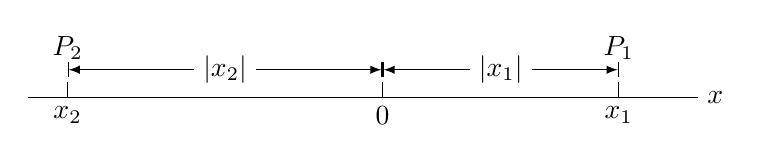
\begin{tikzpicture}[>=latex]
\draw(-.5,0)--(8,0)node[right]{$x$};
\foreach \x/\xtext in {0/x_2,4/0,7/x_1}
{
    \draw (\x,0)node[below]{$\xtext$}--(\x,.2);
}
\draw[|<->|](0,.35)node[above]{$P_2$}--node[fill=white]{$|x_2|$}(4,.35);
\draw[|<->|](7,.35)node[above]{$P_1$}--node[fill=white]{$|x_1|$}(4,.35);

 \end{tikzpicture}
    \caption{}\label{fig:distance}
\end{figure}

如果我们要在 $x$ 轴上描述距离原点不超过 2 个单位的点集,我们把这个条件可以直接写成
\begin{equation}
  \label{eq:abs_neq}
    |x|\leqslant 2
\end{equation}
这个不等式的解集是位于以原点 $O$ 为中心,长度等于 4 的线段上的一切点。\cref{fig:range} 说明这些点的位置。
\begin{figure}
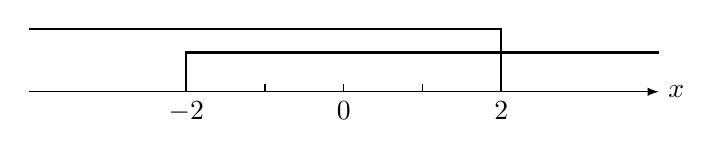
\begin{tikzpicture}[>=latex]
    \draw[->](-4,0)--(4,0)node[right]{$x$};
    \foreach \x in {-2,0,2}
    {
        \draw(\x,0)node[below]{$\x$}--(\x,.1);
    }
    \draw[thick] (-2,0)--(-2,.5)--(4,.5);
    \draw[thick] (2,0)--(2,.8)--(-4,.8);
    \foreach \x in {-1,1}
    {
        \draw(\x,0)--(\x,.1);
    }
\end{tikzpicture}
    \caption{}\label{fig:range} 
\end{figure}

从上面看出这些点的坐标满足不等式
\begin{equation}
  \label{eq:range_neq}
    -2\leqslant x\leqslant 2
\end{equation}
这就是说\cref{eq:abs_neq} 和\cref{eq:range_neq} 是等价的不等式。今后我们将经常遇到的不等式具有下面的形式
\begin{equation}
  \label{eq:abs_neq2}
    |x-a|<3
\end{equation}

$|x-a|=\sqrt{(x-a)^2}$ 的几何意义是 $x$ 轴上的 $P(x,0)$ 点离开 $A(a,0)$ 点的距离。因此已给的不等式是描述在 $x$ 轴上距离 $A(a,0)$ 点小于 3 个单位的点集,根据上面的例题的结论,\cref{eq:abs_neq2} 等价于 $-3<x-a<3$。

不等式的各端加 $a$,得到
\begin{equation}
  a-3<x<a+3    
\end{equation}

因此满足不等式 \eqref{eq:abs_neq2} 的点的坐标是在 $a-3$ 与 $a+3$ 之间(不包括 $a-3$ 和 $a+3$)。

\begin{example}
  在 $x$ 轴上哪些点满足不等式 $|x-3|\leqslant 5$。
\end{example}

\begin{solution}
  $|x-3|\leqslant 5$, 即 $-5\leqslant x-3\leqslant 5$,也即
\[-5+3\leqslant x\leqslant 5+3\]
$\therefore\quad -2\leqslant x\leqslant 8$

这些点位于以 3 为中心,长度等于 10 个单位的线段上,见\cref{fig:solution}。
\begin{figure}
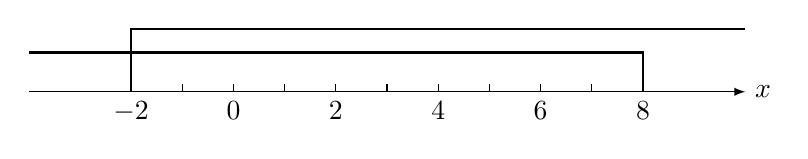
\begin{tikzpicture}[>=latex, xscale=1.3]
    \draw[->](-2,0)--(5,0)node[right]{$x$};
    \foreach \x in {-2,0,2,...,8}
    {
        \draw(\x/2,0)node[below]{$\x$}--(\x/2,.1);
    }
    \foreach \x in {-1,1,...,7}
    {
        \draw(\x/2,0)--(\x/2,.1);
    }
    \draw[thick] (-1,0)--(-1,.8)--(5,.8);
    \draw[thick] (4,0)--(4,.5)--(-2,.5);
\end{tikzpicture}

    \caption{}\label{fig:solution}
\end{figure}

同样地,我们也可以解释 $x>3$ 的几何意义,不等式 $|x|>3$ 是描述在 $x$ 轴上距离原点大于 3 个单位的点集,\cref{fig:solution2} 说明了这些点的位置,图中的圆圈表示去掉 $\pm 3$,因此这些点的坐标小于 $-3$ 或大于 3,即
\[x<-3,\quad \text{或}\quad x>3\]

\begin{figure}
\begin{tikzpicture}[>=latex]
    \draw[->](-4,0)--(4,0)node[right]{$x$};
    \foreach \x in {-3,0,1,3}
    {
        \draw(\x,0)node[below]{$\x$}--(\x,.1);
    }
    \foreach \x in {-2,-1,...,2}
    {
        \draw(\x,0)--(\x,.1);
    }
    \draw[thick] (-3,0)--(-3,.5)--(-4,.5);
    \draw[thick] (3,0)--(3,.5)--(4,.5);
    \foreach \x in {-3,3}
    {
        \draw (\x,0) [fill=white]circle(1.5pt);
    }
\end{tikzpicture}
    \caption{}\label{fig:solution2}
\end{figure}

这就是说,不等式 $|x|>a\; (a>0)$ 等价于不等式 $x<-a$ 或 $x>a\; (a>0)$。
\end{solution}


\begin{example}
  求满足不等式 $(x+2)^2-16>0$ 的点集。
\end{example}

\begin{solution}
  移项
  \[(x+2)^2>16\]
  两边开平方,等价于
  \[|x+2|>4\]
  即
  \[\begin{split}
        x+2<-4\qquad &\text{或}\qquad x+2>4\\  x<-6\qquad &\text{或}\qquad x>2
  \end{split}\]
因此,满足不等式的解集是 $\{x|x<-6\}\cup\{x|x>2\}$。

利用二次函数 $y=(x+2)^2-16$ 的草图,如\cref{fig:parabolic},就更直接地得到 $x<-6$或$x>2$。
\begin{figure}
\begin{tikzpicture}[>=latex, scale=.5]
    \draw[->](-7,0)--(3,0)node[right]{$x$};
    \draw[->](0,-17)--(0,1)node[right]{$y$}; 
\draw[domain=-6.1:2.1, samples=100, thick] plot(\x,{(\x+2)*(\x+2)-16 });
\foreach \y in {-1,-2,...,-16}
{
    \draw (0,\y)--(-.2,\y);
}
\foreach \x in {-6,-5,...,2}
{
    \draw (\x,0)--(\x,.2);
}
\node at (2.5,0)[below]{$2$};
\node at (-6.5,0)[below]{$-6$};
\node at (.5,-.5){$O$};
\node at (0,-16)[right]{$-16$};
\end{tikzpicture}
    \caption{}\label{fig:parabolic}
\end{figure}
\end{solution}

\subsubsection{和、积、商的绝对值}
若 $a$ 和 $b$ 是实数,则 $a\leqslant |a|$ 和 $b\leqslant |b|$,相加得到
\[a+b\leqslant  |a|+|b|\]
同样
\[-a\leqslant |a|\qquad \text{和}\qquad -b\leqslant |b|\]
于是
\[-a-b\leqslant |a|+|b|\]
因为 $a+b$ 和 $-(a+b)$ 都不大于 $|a|+|b|$,所以这两个数中最大者也不大于$|a|+|b|$,于是
\[|a+b|=\max\{a+b,-(a+b)\}\leqslant |a|+|b|\]
这个结果
\begin{equation}
    |a+b|\leqslant |a|+|b|
\end{equation}
常叫做\emph{三角不等式},因为它类似于三角形中任何一边小于其它两边之和这个定理。

有时,我们需要 $|a+b|$ 的下限估值,注意到
\[|a|=|(a+b)-b| \leqslant |a+b| +|-b| =|a+b| +|b|\]
因此下面不等式成立
\begin{equation}
  |a+b|\geqslant |a|-|b|
\end{equation}

若 $a,b$ 是任何实数,则
\[|ab|=\sqrt{(ab)^2}=\sqrt{a^2b^2}=\sqrt{a^2}\cdot \sqrt{b^2}=|a|\cdot |b|\]
即
\begin{equation}
  |ab|=|a|\cdot |b|
\end{equation}
\[\left|\frac{a}{b}\right|=\sqrt{\left(\frac{a}{b}\right)^2}=\sqrt{\frac{a^2}{b^2}}=\frac{\sqrt{a^2}}{\sqrt{b^2}}=\frac{|a|}{|b|}\]
即
\begin{equation}
    \left|\frac{a}{b}\right|=\frac{|a|}{|b|}
\end{equation}


\begin{Exercise}
\begin{question}
  \item 解不等式组:
    \[\begin{cases}
      \dfrac{x}{2}-\dfrac{x}{3}>-1\\
      2(x-3)-3(x-2)<0
    \end{cases}\]
  \item 解不等式:
  \begin{tasks}(2)
      \task $|2x-1|<2|1-2x|-3$
      \task $|x+1|+|x-5|>3$
      \task $\left|\dfrac{3x}{x+1}-3\right|<0.01$
      \task $\dfrac{3x-1}{x-5}<2$
  \end{tasks}
  \item 图示满足下面不等式组的点 $(x,y)$的区域 $R$。
  \[\begin{cases}
      |x-1|+|y-5|<1\\
  y>5+|x-1|
  \end{cases}\]
  \item 试证明若 $ax^2+bx+c>0$ 对于任何 $x$ 都成立的充要条件是 $a>0$ 且 $b^2-4ac<0$。
  \item 等差数列与等比数列的首项相等且第 $2n+1$ 项也相等,问第 $n+1$ 项如何?
  \item 若 $x+2y=1$, 求 $xy$ 的最大值。
  \item 平移 $y=-\dfrac{1}{3}x^2$ 使其顶点在抛物线 $y=x^2$ 上,试求这样得到任何一条抛物线都不能经过的范围,并画图表示。
  \item 求证
  \begin{tasks}
    \task $|a+b+c|\leqslant |a|+|b|+|c|$
    \task $|a-b-c|\geqslant |a|-|b|-|c|$
    \task $\Big| |a|-|b| \Big|\leqslant |a+b|$
  \end{tasks}
  \item \begin{tasks}
    \task 若 $|h|<\frac{\varepsilon}{4}$,$|k|<\frac{\varepsilon}{6}$,求证 $|2h-3k|<\varepsilon$。
    \task 若 $|a_n-r|<\varepsilon$,$|a_n-a_n'|<\varepsilon$,求证 $|a_n'-r|<\varepsilon$。
    \task 若 $|b_n|<\varepsilon$,$|a_n-b_n|<\varepsilon$,求证 $|a_n|<2\varepsilon$。
  \end{tasks}
  \item 试用 $a$ 表出从点 $(0,a)$ 到曲线 $y=\left|\frac{x^2}{2}-1\right|$ 上的点 $(x,y)$ 的距离的最小值 $(a>1)$。
  \item 解不等式 $\sqrt{2x^2-3x-2}>x-1$。
\end{question}
\end{Exercise}

\subsection{几个重要的不等式}
下面我们来推导几个常用的著名不等式。

\begin{example}\label{exp:bernoulli}
  贝努利不等式。若 $n\in\mathbb{N}$且$n\geqslant 2$, $a>-1$ 且 $a \neq 0$(即 $a>0$ 或 $-1<a<0$ ),则
\[(1+a)^n>1+na\]
\end{example}

\begin{proof}
\begin{enumerate}
  \item 对于 $n=2$, 因为 $(1+a)^2=1+2a+a^2$,又 $a^2>0$,故不等式成立。
  \item 假设不等式对于 $n=k$ 成立,即
  \[(1+a)^k>1+ka\]
  我们来证明不等式对于 $n=k+1$ 也成立,就是说
  \[(1+a)^{k+1}>1+(k+1)a\]

  事实上,由假设 $1+a>0$,故不等式
  \[(1+a)^k(1+a)>(1+ka)(1+a)\]
  成立,即
  \[(1+a)^{k+1}>1+(k+1)a+ka^2\]
  将上面不等式右边舍去正项 $ka^2$,就知道
  \[(1+a)^{k+1}>1+(k+1)a\]
  成立,因此命题对于 $n\geqslant 2$ 的自然数成立。
\end{enumerate}
\end{proof}

\begin{example}
  无论多少个正数的几何平均数不大于其算术平均数,即
\[\frac{a_1+a_2+\cdots+a_n}{n}\geqslant \sqrt[n]{a_1a_2\cdots a_n}\]
\end{example}

\begin{proof}
令 $A=\dfrac{a_1+a_2+\cdots+a_n}{n}$,则题意是说,
\begin{equation}
  \label{eq:avg_proof}
  A^n\geqslant a_1a_2\cdots a_n
\end{equation}
当 $a_1=a_2=\cdots= a_n$ 时,则\cref{eq:avg_proof} 显然成立。如果 $a_1,a_2,\ldots,a_n$ 这 $n$ 个数有不相等的,由于
    \[nA=a_1+a_2+\cdots+a_n\]
即:
\[(a_1-A)+(a_2-A)+\cdots+(a_n-A)=0\]
则必有一大于 $A$, 也必有一小于 $A$, 不妨设 $a_1>A>a_2$,于是,$A-a_1<0$,$A-a_2>0$,把 $a_1,a_2,\ldots,a_n$ 改换成
\begin{equation}
  \label{eq:new_series}
a_1'=A,\; a_2'=a_2+a_1-A,\; a_3'=a_3,\; \ldots, a_n'=a_n
\end{equation}
由此可见我们新得之 $n$ 个数,其和不变,即
\[\begin{split}
    a'_1+a'_2+\cdots +a'_n&=A+(a_2+a_1-A)+a_3+\cdots +a_n\\
&= a_1+a_2+\cdots +a_n\\
&=nA
\end{split}\]
但其积增大,因为
\[\begin{split}
    A(a_2+a_1-A)-a_1a_2&=Aa_2+Aa_1-A^2-a_1a_2\\
&=A(a_2-A)+a_1(A-a_2)\\
&=(A-a_2)(a_1-A)>0
\end{split}\]
从而
\[A(a_2+a_1-A)a_3\cdots a_n>a_1a_2\cdots a_n\]
若\cref{eq:new_series} 中还有不等于 $A$ 的,比如,$a_s>A>a_m$,我们用同法即用 $A$ 取代其中较大的一个 $a_c$,用 $a_m+a_s-A$ 代换 $a_m$,又可另得 $n$ 个正数,其和同前,而其积更大。由此以往,不过 $n-1$ 次,便可得 $n$ 个相等之正数$\underbrace{A,A,\cdots A}_{\text{$n$个}}$,此时积最大,故有
\[A^n\geqslant a_1a_2\cdots a_n\]
且当 $a_1=a_2=\cdots =a_n$ 时,等式成立。
\end{proof}

\begin{example}\label{exp:Cauchy}
  柯西不等式,若 $a_i,b_i,\; i=1,2,\cdots ,n$ 是实数,则
\[(a_1b_1+a_2b_2+\cdots +a_nb_n)\leqslant (a_1^2+a_2^2+\cdots +a_n^2)(b_1^2+b_2^2+\cdots+b_n^2)\]
当且仅当
$\dfrac{a_1}{b_1}=\dfrac{a_2}{b_2}=\cdots=\dfrac{a_n}{b_n}$ 时,等式成立。
\end{example}

\begin{proof}
对于任何实数 $t$, 不等式
\begin{equation}
  \label{eq:cauchy_binom}
  (a_1+tb_1)^2+(a_2+tb_2)^2+\cdots +(a_n+tb_n)^2\geqslant 0
\end{equation}
成立,将\cref{eq:cauchy_binom} 的左端改写成按 $t$ 的降幂排列,得
\begin{equation}
  \label{eq:cauchy_binom2}
   ( b^2_1+b^2_2+\cdots +b^2_n)t^2+2(a_1b_1+\cdots +a_nb_n)t+(a^2_1+a_2^2+
+\cdots +a_n^2)\geqslant 0
\end{equation} 
设 $A=a^2_1+\cdots +a_n^2$,$B=a_1b_1+\cdots +a_nb_n$,$C=b^2_1+\cdots +b^2_n$,
于是\cref{eq:cauchy_binom2} 写成 $Ct^2+2Bt+A>0$,其中 $C\geqslant 0$。
\begin{itemize}
  \item 若 $C=0$, 于是 $b_1=b_2=\cdots =b_n=0$,显然,柯西不等式成立。
  \item 若 $C>0$,因而 
  \[C\left(t+\frac{B}{C}\right)^2+\left(A-\frac{B^2}{C}\right)\geqslant 0\]
  对于任意实数 $t$ 成立。故令 $t=-\dfrac{B}{C}$ 代入,得到
  \[A-\frac{B^2}{C}\geqslant 0,\qquad \text{即}\qquad \frac{AC-B^2}{C}\geqslant 0\]
  $\because\quad C>0,\qquad \therefore\quad B^2\leqslant AC$, 即
\[(a_1b_1+\cdots +a_nb_n)^2\leqslant (a^2_1+\cdots +a^2_n)(b^2_1+\cdots +b^2_n)\]
再由\cref{eq:cauchy_binom} 推知当且仅当 $-t=\dfrac{a_1}{b_1}=\dfrac{a_2}{b_2}=\cdots=\dfrac{a_n}{b_n}$ 时,等式成立。
\end{itemize}
\end{proof}

\begin{example}
  设 $a_1,a_2,\ldots,a_n,b_1,b_2,\ldots,b_n$ 是实数,则
\[\sqrt{\sum^n_{i=1}(a_i+b_i)^2}\leqslant \sqrt{\sum^n_{i=1}a^2_i}+\sqrt{\sum^n_{i=1}b^2_i}\]
\end{example}

\begin{proof}
 \[   \sum^n_{i=1}(a_i+b_i)^2=\sum^n_{i=1}a_i^2+2\sum^n_{i=1}a_ib_i+\sum^n_{i=1}b_i^2\]
由\cref{exp:Cauchy} 柯西不等式知
\[\sum^n_{i=1}a_ib_i\le\left|\sum^n_{i=1}a_ib_i\right|\leqslant \sqrt{\sum^n_{i=1}a_i^2}\sqrt{\sum^n_{i=1}b_i^2}\]
因此:
\[\begin{split}
    \sum^n_{i=1}(a_i+b_i)^2&\leqslant \sum^n_{i=1}a_i^2+2\sqrt{\sum^n_{i=1}a_i^2}\sqrt{\sum^n_{i=1}b_i^2}+\sum^n_{i=1}b_i^2\\
    &=\left(\sqrt{\sum^n_{i=1}a^2_i}+\sqrt{\sum^n_{i=1}b^2_i}\right)^2
\end{split}\]
两边开平方,取算术根即得所证。
\end{proof}    

% \section*{习题6.3}
% \addcontentsline{toc}{subsection}{习题6.3}
\begin{Exercise}
\begin{question}
   \item  若 $a,b,c,d$ 是不相等正数,求证:
\begin{tasks}
    \task $\displaystyle \frac{b}{a}+\frac{c}{b}+\frac{d}{c}+\frac{a}{d}>4$
    \task $\displaystyle \frac{b}{\sqrt{a}}+\frac{a}{\sqrt{b}}>\sqrt{a}+\sqrt{b}$
\end{tasks}
   \item  若 $a_1,a_2$ 表示正数,$p,q$ 表示正整数,求证:
\begin{tasks}
    \task $\displaystyle a_1^{p+q}+a_2^{p+q}\geqslant a_1^pa_2^q+a_1^qa_2^q$
    \task $\displaystyle \frac{a_1^{p+q}+a_2^{p+q}}{2}\geqslant \left(\frac{a_1^p+a_2^p}{2}\right)\left(\frac{a_1^q+a_2^q}{2}\right)$
\end{tasks}

\item 用数学归纳法证明:
若 $a_1>0$,$a_2>0$,$n$ 是正整数,则
\[\frac{a_1^n+a_2^n}{2}\geqslant \left(\frac{a_1+a_2}{2}\right)^n\]
\item 求证,当 $n$ 是 1 或不小于 5 的自然数时,总有 $2^n>n^2$。
\item 设 $0<a<1$,$0<x_0<1$,$x_n=a(1-x_{n-1})+(1-a)x_{n-1},\quad (n=1,2,3,\ldots)$,
\begin{tasks}
  \task 用 $a$ 与 $x_0$ 表示 $x_n$;
  \task 证明 $0<x_n<1$。
\end{tasks}

\item 设 $a>2$,给定数列 $\{x_n\}$,其中$x_1=a$,$x_{n+1}=\dfrac{x^2_n}{2(x_n-1)},\quad (n=1,2,3,\ldots)$,
求证:
\begin{tasks}
  \task $x_n>2$,且$\dfrac{x_{n+1}}{x_n}<1$;
  \task 如果 $a<3$,那么 $x_n\leqslant 2+\dfrac{1}{2^{n-1}}$。
\end{tasks}

\item 若长方形的体积是定值,求全面积的最小值。
\item 求证球内接长方体中,以正方体的体积为最大。
\item 求证在周长都为 $2L$ 的所有三角形中,面积最大的必是等边三角形。
\item 若 $a,b,c$ 是正数且 $abc=8$。

求证:$\sqrt{a^2+b^2}+\sqrt{b^2+c^2}+\sqrt{c^2+a^2}\geqslant 6\sqrt{2}$

\item 若$a>0$, $b>0$, 且$a+b=1$, 
求证:\[\left(a+\frac{1}{a}\right)\left(b+\frac{1}{b}\right)\geqslant \frac{25}{4}\]

\item 若 $a+b+c=1$, 且 $a>0$, $b>0$, $c>0$, 求证:
\begin{tasks}
    \task $\displaystyle \left(\frac{1}{a}-1\right)\left(\frac{1}{b}-1\right)\left(\frac{1}{c}-1\right)\geqslant 8$
    \task $\displaystyle \frac{1}{a}+\frac{1}{b}+\frac{1}{c}\geqslant 9$
\end{tasks}

\item 若 $x,y$ 是实数,且 $x^2+y^2\leqslant 1$,
求证:$|x^2+2xy-y^2|\leqslant \sqrt{2}$

\item 对于任何实数,求证:
\[\sqrt{\frac{a_1^2+a_2^2+\cdots+a_n^2}{n}}\geqslant \frac{a_1+a_2+\cdots+a_n}{n}\]
当且仅当诸数相等时,等式成立。
\item $a+b=1$, $a>0$, $b>0$, 求证 $\sqrt{2a+1}+\sqrt{2b+1}\leqslant 2\sqrt{2}$。
\item 求证:
\[\frac{|x_1+x_2|}{|4+x_1^2| |4+x_2^2|}<\frac{1}{8}\]
\item 对于 $n\geqslant 2$ 的自然数 $n$, 证明不等式
\[2^n>1+n\sqrt{2^{n-1}}\]
\item 对于任何正整数 $k\leqslant n$, 求证:
\[1+\frac{k}{n}\leqslant \left(1+\frac{1}{n}\right)^k\leqslant 1+\frac{k}{n}+\frac{k^2}{n^2}\]
\item 已知 $a,b,c,d,e$ 是实数,满足
\[a+b+c+d+e=8,\qquad a^2+b^2+c^2+d^2+e^2=16\]
试确定 $e$ 的最大值。
\item 半径为 1 的圆内接三角形面积等于 $\dfrac{1}{4}$,设此三角形三边长为 $a,b,c$,求证:
\begin{tasks}
  \task $abc=13$;
  \task $\sqrt{a}+\sqrt{b}+\sqrt{c}<\dfrac{1}{a}+\dfrac{1}{b}+\dfrac{1}{c}$。
\end{tasks}

\item 直角三角形斜边长等于10, 内切圆半径为$a$。求何
时内切圆的半径最大,最大值是多少?
\item 若$n>2$, 求证$(n!)^2>n^n$。
\item 有$n$个实数$a_1,a_2,\ldots,a_n$且
$a_1+a_2+\cdots+a_n=n$
\begin{tasks}
  \task 求证:$\sqrt{|a_1|}+\sqrt{|a_2|}+\cdots+\sqrt{|a_n|}\geqslant \sqrt{n}$
  \task 又 $a^2_1+a_2^2+\cdots+a^2_n=n$,求 $a_1,a_2,\ldots,a_n$ 的值。
\end{tasks}

\item 若 $a,b,c$ 是正实数,求证:$\dfrac{c}{a+b}+\dfrac{a}{b+c}+\dfrac{b}{c+a}\geqslant \dfrac{3}{2}$。
\end{question}
\end{Exercise}


\input{contents/4-07.tex}
\input{contents/4-08.tex}
\chapter{反三角函数与简单三角方程的解法}
\section{反正弦函数}
我们知道,正弦函数$y=\sin x$是一个周期等于$2\uppi$的振动函
数,它的定义域是$(-\infty,+\infty)$, 而值域是闭区间$[-1,1]$, 它的图象如图9.1。

\begin{figure}[htp]
    \centering
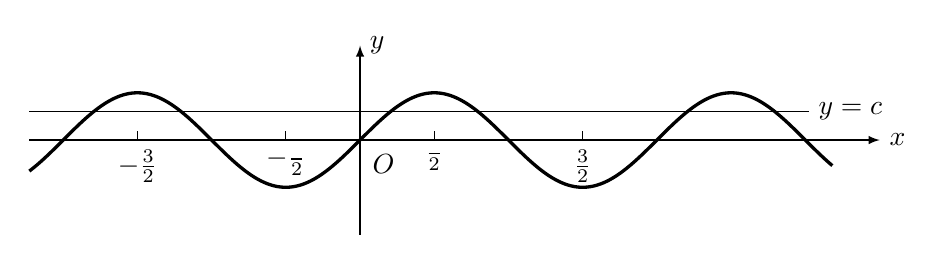
\begin{tikzpicture}[>=latex, scale=.6]
\draw[->] (-7,0)--(11,0)node[right]{$x$};
\draw [->] (0,-2)--(0,2)node[right]{$y$};

\draw[domain=-7:10, samples=1000, very thick] plot(\x,{sin(\x r)});
\draw  (-7,.6)--(9.5,0.6)node[right]{$y=c$};

\foreach \x/\xtext in {-1.5*pi/-\frac{3\uppi}{2}, -.5*pi/-\frac{\uppi}{2},.5*pi/\frac{\uppi}{2}, 1.5*pi/\frac{3\uppi}{2}}
{
    \draw (\x,0)node[below]{$\xtext$}--(\x,.2);
}
\node at (.5,-.5){$O$};
\end{tikzpicture}
    \caption{}
\end{figure}


每取一数$y=c,\; -1\leqslant c\leqslant 1$, 作直线$y=c$, 可与正弦曲线
$y=\sin x$交于无穷多个点,这些交点的横坐标是
\[x=x_0+2k\uppi\qquad \text{和}\qquad x=(\uppi -x_0)+2k\uppi\quad (k\in\mathbb{Z})\]
因此有无数多个$x$的值满足方程$\sin x =c$, 而和那个$y=c$对
应。可见对于变数$x$的一切可能实数值来说,我们不能由函
数$f:\mathbb{R}\to [-1,1]$, $f(x)=\sin x$得出它的反函数来。把定
义域分成无数个单调区间,则在各区间$\left[-\frac{\uppi}{2}+2k\uppi, \frac{\uppi}{2}+2k\uppi\right]$上,$y=\sin x$由$-1$上升到1,而在各区间$\left[\frac{\uppi}{2}+2k\uppi, \frac{3\uppi}{2}+2k\uppi\right]$上,$y=\sin x$由1下降到$-1$,于是由前一章中的
反函数定理知道,对于上述每一个单调区间存在一个反函数。

如果我们强调的是在闭区间$\left[-\frac{\uppi}{2},\frac{\uppi}{2}\right]$上
来考虑正弦
函数的反函数,我们就说它是反正弦函数的主值,并把这个函数记作
$x=\arcsin y$,使得
$$x=\arcsin y\qquad \Longleftrightarrow \qquad y=\sin x$$
这里$x\in \left[-\frac{\uppi}{2},\frac{\uppi}{2}\right],\quad y\in[-1,+1]$。

对于使得$y=\sin x$是单调的另一区间,例如$x\in \left[\frac{\uppi}{2},\frac{3\uppi}{2}\right]$,
我们就得到另一个反正弦函数。假如我们没有明确地指出反正弦函数的值域所在的区间,我们就不能由函数 $y=\sin x$ 得出它的反函数。为了明确起见,现在我们规定

\begin{Definition}%{定义1}
函数 $y=\sin x$ 在闭区间 $\left[-\frac{\uppi}{2},\frac{\uppi}{2}\right]$ 上
的反函数叫做\emph{反正弦函数}或\emph{反正弦},这个函数用记号写作
$x=\arcsin y$ (即$x$是一角或弧,其相应的正弦值为$y$),
它的定义域是闭区间$-1\leqslant y\leqslant 1$, 值域是闭区间$-\frac{\uppi}{2}\leqslant x\leqslant \frac{\uppi}{2}$。
\end{Definition}

用习惯上的写法,将字母 $x$ 与 $y$ 互换而写成 $y=\arcsin x$,
现在,我们将反正弦函数(主值)的定义用几何名词叙述如下:

在闭区间 $-1\leqslant x\leqslant 1$ 上,数 $x$ 的反正弦 $y=\arcsin x$ 是在
闭区间 $\left[-\frac{\uppi}{2},\frac{\uppi}{2}\right]$ 上的一个角或弧,它的正弦值等于 $x$,即 $\sin y=x$。

由反正弦函数的定义和前一章的反函数定理可得到
它的一些性质如下:
\begin{itemize}
    \item $\arcsin(\sin y)=y,\qquad -\frac{\uppi}{2}\leqslant y\leqslant \frac{\uppi}{2}$
    
    $\sin(\arcsin x)=x,\qquad -1\leqslant x\leqslant 1$

    \item 函数$f(x)=\arcsin x$在闭区间$[-1,1]$上单调递
    增,并且连续。
    \item $y=\arcsin x,\; -1\leqslant x\leqslant 1$的图象与$y=\sin x,\; -\frac{\uppi}{2}\leqslant y\leqslant \frac{\uppi}{2}$
    的图象关于直线$y=x$对称(图5.2)。
\end{itemize}

\begin{figure}[htp]
    \centering
\begin{tikzpicture}[>=latex, scale=1]
\draw[->] (-4,0)--(4,0)node[right]{$x$};
\draw [->] (0,-3)--(0,3)node[right]{$y$};

\draw[domain=-pi:pi, samples=1000, dashed, thick] plot(\x,{sin(\x r)});
\draw[domain=-1:1, samples=1000, very thick] plot(\x,{asin(\x)*pi/180});
\draw[dashed] (-3,-3)--(2.5,2.5)node [above]{$y=x$};
\draw [dashed] (0,.5*pi)node[left]{$\frac{\uppi}{2}$}--(1,.5*pi)node[above]{$y=\arcsin x$};
\draw [dashed] (0,-.5*pi)node[right]{$-\frac{\uppi}{2}$}--(-1,-.5*pi);
\node at (.25,-.25){$O$};
\node at (pi+.5,0)[above]{$y=\sin x$};
\foreach \x in {-1,1}
{
    \draw (\x,0)node[below]{$\x$}--(\x,.1);
}
\draw (0,1)node[left]{$1$}--(.1,1);
\draw (0,-1)--(-.1,-1)node[right]{$-1$};

\end{tikzpicture}
    \caption{}
\end{figure}



我们已知正弦函数是奇函数,它的图象关于原点对称,
现在我们要证明 $f(x)=\arcsin x$是奇函数,即
$\arcsin(-x)=-\arcsin x$。

\begin{proof}
    因为$-\frac{\uppi}{2}\leqslant \arcsin x\leqslant \frac{\uppi}{2}$,
    角$-\arcsin x$也被限制在由$-\frac{\uppi}{2}$到$\frac{\uppi}{2}$
    的区间内:
    $$-\frac{\uppi}{2}\leqslant -\arcsin x\leqslant \frac{\uppi}{2}$$
    又,角$-\arcsin x$的正弦等于$-x$
\[\sin(-\arcsin x)=-\sin(\arcsin x)=-x\]
因此:$\arcsin(-x)=-\arcsin x$。
\end{proof}

\begin{example}
    求下列各式的值(口答):
    \begin{enumerate}
        \item $\arcsin\frac{1}{2}$
        \item $\arcsin\left(-\frac{1}{2}\right)$
        \item $\arcsin 1$
    \end{enumerate}
\end{example}

\begin{solution}
\begin{enumerate}
    \item $\arcsin\frac{1}{2}=\frac{\uppi}{6}$,因为$\sin\frac{\uppi}{6}=\frac{1}{2}$,且$-\frac{\uppi}{2}<\frac{\uppi}{6}<\frac{\uppi}{2}$

    \item $\arcsin\left(-\frac{1}{2}\right)=-\frac{\uppi}{6}$,因为$\sin\left(-\frac{\uppi}{6}\right)=-\frac{1}{2}$,且
    $-\frac{\uppi}{2}<-\frac{\uppi}{6}<\frac{\uppi}{2}$
    \item $\arcsin 1=\frac{\uppi}{2}$,因为$\sin\frac{\uppi}{2}=1$,而且$\frac{\uppi}{2}$不超出$\left[-\frac{\uppi}{2},\frac{\uppi}{2}\right]$的界限。
\end{enumerate}
\end{solution}

\begin{example}
    求下列各式的值:
\[\arcsin\left(-\frac{\sqrt{3}}{2}\right),\qquad \arcsin (-0.2672) \]
\end{example}

\begin{solution}
\begin{enumerate}
    \item $\arcsin\left(-\frac{\sqrt{3}}{2}\right)=-\arcsin\frac{\sqrt{3}}{2}=-\frac{\uppi}{3}$
    \item $\arcsin(-0.2672)=-\arcsin0.2672=-15^{\circ}30'\approx -0.2705$
\end{enumerate}
    
\end{solution}



\begin{example}
    求下列各式的值:
\begin{tasks}(2)
  \task $\sin\left(\arcsin\frac{1}{3}\right)$
  \task $\tan\left(\arcsin\frac{\sqrt{2}}{2}\right)$
  \task $\cos\left(\arcsin\frac{3}{5}\right)$
  \task $\sin\left[2\arcsin\left(-\frac{3}{5}\right)\right]$
  \task $\arcsin\left(\sin\frac{7\uppi}{6}\right)$
\end{tasks}
\end{example}

\begin{solution}
\begin{enumerate}
    \item $\sin\left(\arcsin\frac{1}{3}\right)=\frac{1}{3}$
    \item $\tan\left(\arcsin\frac{\sqrt{2}}{2}\right)=\tan\frac{\uppi}{4}=1$
    \item 设$\arcsin\frac{3}{5}=\alpha$,其中$-\frac{\uppi}{2}\le\alpha\le\frac{\uppi}{2}$,那么$\sin\alpha=\frac{3}{5}$。由于$-\frac{\uppi}{2}\le\alpha\le\frac{\uppi}{2}$,$\sin\alpha>0$,可以知道,$\alpha$是第一象限的角,所以
    $$\cos\left(\arcsin\frac{3}{5}\right)=\sqrt{1-\left(\frac{3}{5}\right)^2}=\frac{4}{5}$$
    \item 设$\arcsin\left(-\frac{3}{5}\right)=\alpha$,其中$-\frac{\uppi}{2}\le\alpha\le\frac{\uppi}{2}$,那么
    \[\sin\alpha =\sin\left[\arcsin\left(-\frac{3}{5}\right)\right]=-\frac{3}{5}\]
由于$-\frac{\uppi}{2}\le\alpha\le\frac{\uppi}{2}$和$\sin\alpha<0$,可以知道$\alpha$是第四象限的角,所以
\[\cos\alpha=\sqrt{1-\left(-\frac{3}{5}\right)^2}=\frac{4}{5}\]
即:
$\sin\left[2\arcsin\left(-\frac{3}{5}\right)\right]=\sin2\alpha=2\sin\alpha\cdot \cos\alpha=2\left(-\frac{3}{5}\right)\cdot\left(\frac{4}{5}\right)=-\frac{24}{25}$
    \item \[\begin{split}
\arcsin\left(\sin\frac{7\uppi}{6}\right)&=\arcsin\left[\sin\left(\uppi+\frac{\uppi}{6}\right)\right]\\
&=\arcsin\left(-\sin\frac{\uppi}{6}\right)\\
&=-\arcsin\left(\sin\frac{\uppi}{6}\right)=-\frac{\uppi}{6}        
    \end{split}\]
\end{enumerate}
\end{solution}

关于 $y=\sin x$, 只要知道了它在闭区间 $-\frac{\uppi}{2}\leqslant x\leqslant \frac{\uppi}{2}$ 上
的反函数 $x=\arcsin y$,我们便能求出 $y=\sin x$ 在其它单调区间上的反函数。

\begin{Theorem}{命题}
\begin{enumerate}
    \item $y=\sin x$在闭区间$\left[-\frac{\uppi}{2}+2k\uppi,\frac{\uppi}{2}+2k\uppi\right]$上,由$-1$上升到1,它们相应的反函数是
\[x=\arcsin y+2k\uppi,\quad k\in\mathbb{Z}\]
因为
\[\sin x= \sin(\arcsin y+ 2k\uppi) = \sin(\arcsin y) = y\]
而且
\[-\frac{\uppi}{2}+2k\uppi\leqslant \arcsin y+2k\uppi \leqslant \frac{\uppi}{2}+2k\uppi
,\quad k\in\mathbb{Z}\]
    
\item\label{itm:arcsin_case2} $y=\sin x$在闭区间$\left[\frac{\uppi}{2},\frac{3\uppi}{2}\right]$上,由1下降到$-1$,
它的反函数是
\[x=\uppi-\arcsin y\]
因为
\[\sin x=\sin(\uppi- \arcsin y) = \sin(\arcsin y) = y\]
而且
\[\frac{\uppi}{2}=\uppi-\frac{\uppi}{2} \leqslant \uppi-\arcsin y \leqslant \uppi+\frac{\uppi}{2}=\frac{3\uppi}{2}\]
我们也可以在单位圆上作图来说明 \ref{itm:arcsin_case2},如图9.3所示。

\item $y=\sin x$ 在闭区间 $\left[\dfrac{\uppi}{2}+2k\uppi,\dfrac{3\uppi}{2}+2k\uppi\right]$上,由
1下降到$-1$, 相仿地证得它在相应区间上的反函数是
\[x=(\uppi-\arcsin y)+2k\uppi,\quad k\in\mathbb{Z} \]
\end{enumerate}
\end{Theorem}

\begin{figure}[htp]
    \centering
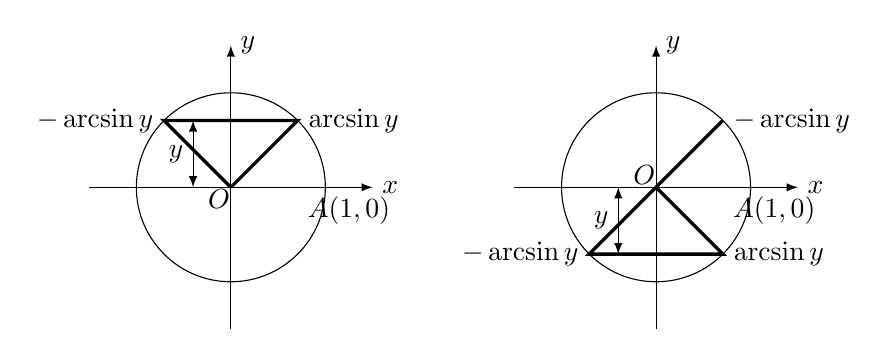
\begin{tikzpicture}[>=latex, scale=.6]
\begin{scope}
    \draw[->] (-3,0)--(3,0)node[right]{$x$};
    \draw[->] (0,-3)--(0,3)node[right]{$y$};
    \draw (0,0) circle(2);
    \node at (-.25,-.25){$O$};
\node at (2.5,0)[below]{$A(1,0)$};
\draw[very thick] (0,0)--(45:2)node[right]{$\arcsin y$}--(90+45:2)node[left]{$\uppi-\arcsin y$}--(0,0);

\draw[<->] (-.8,0)--node[left]{$y$}(-.8,1.414);
\end{scope}

\begin{scope}[xshift=9cm]
    \draw[->] (-3,0)--(3,0)node[right]{$x$};
    \draw[->] (0,-3)--(0,3)node[right]{$y$};
    \draw (0,0) circle(2);
    \node at (-.25,.25){$O$};
\node at (2.5,0)[below]{$A(1,0)$};

\draw[<->] (-.8,0)--node[left]{$y$}(-.8,-1.414);
\draw[very thick] (0,0)--(-45:2)node[right]{$\arcsin y$}--(-90-45:2)node[left]{$\uppi-\arcsin y$}--(0,0);
\draw[very thick] (0,0)--(45:2)node[right]{$-\arcsin y$};
\end{scope}
\end{tikzpicture}

    \caption{}
\end{figure}


\begin{example}
  讨论函数 $y=\arcsin(\sin x)$ 的图象。
\end{example}

\begin{solution}
  由于正弦的周期性,函数 $\arcsin(\sin x),\; x\in\mathbb{R}$ 也以 $2\uppi$ 为周期,因此,只研究它在长度为 $2\uppi$ 的区间内情形即可。由于
  \[\sin y=\sin[\arcsin(\sin x)]=\sin x\]
  这里 $-\frac{\uppi}{2}\leqslant y\leqslant \frac{\uppi}{2}$,而 $x\in\mathbb{R}$,故
  \begin{itemize}
    \item 当 $x\in\left[-\frac{\uppi}{2},\frac{\uppi}{2}\right]$ 时,则 $y=x$。
    \item 当 $x\in\left[\frac{\uppi}{2},\frac{3\uppi}{2}\right]$ 时,则由上面的命题 2 知
    \[x=\uppi-y\quad \Rightarrow\quad y=\uppi-x\in \left(-\frac{\uppi}{2},\frac{\uppi}{2}\right)\]
  \end{itemize}
因之,在此区间内函数的图象与直线 $y=\uppi-x$ 一致,总之,由上面的命题中的 1 和 3 的结果:
\begin{enumerate}
  \item 当$x\in \left[-\frac{\uppi}{2}+2k\uppi,\frac{\uppi}{2}+2k\uppi\right]$时,则$x=y+2k\uppi$,则$y=x-2k\uppi$;
  \item 当$x\in \left[\frac{\uppi}{2}+2k\uppi,\frac{3\uppi}{2}+2k\uppi\right]$时,则$x=\uppi-y+2k\uppi$,则$y=(\uppi-x)-2k\uppi$。
\end{enumerate}
由上面讨论的结果,得到函数 $y= \arcsin(\sin x)$ 的图象是折线的形状,如图 5.4所示。
\begin{figure}[htp]
    \centering
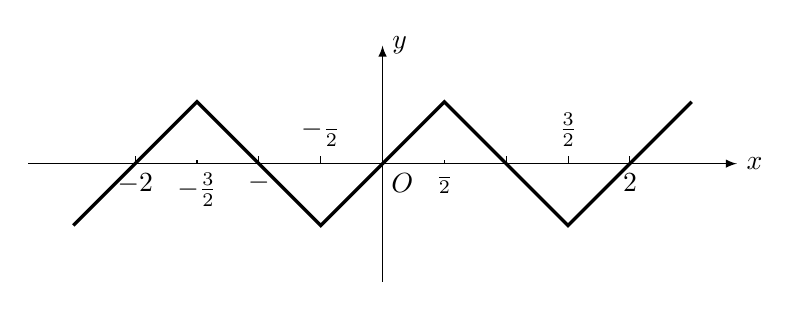
\begin{tikzpicture}[>=latex, scale=.5]
    \draw[->] (-9,0)--(9,0)node[right]{$x$};
    \draw[->] (0,-3)--(0,3)node[right]{$y$};
\draw[very thick] (-2.5*pi,-0.5*pi)--(-1.5*pi,.5*pi)--(-.5*pi,-0.5*pi)--(.5*pi,.5*pi)--(1.5*pi,-0.5*pi)--(2.5*pi,.5*pi);
\foreach \x/\xtext in {-2/-2\uppi, -1/-\uppi,1/\uppi,2/2\uppi}
{
    \draw (pi*\x,0)node[below]{$\xtext$}--(pi*\x,0.2);
}
\foreach \x/\xtext in {.5/\frac{\uppi}{2},-1.5/-\frac{3\uppi}{2}}
{
    \draw (pi*\x,0)node[below]{$\xtext$}--(pi*\x,0.1);
}
\foreach \x/\xtext in {1.5/\frac{3\uppi}{2},-.5/-\frac{\uppi}{2}}
{
    \draw (pi*\x,0)--(pi*\x,0.2)node[above]{$\xtext$};
}
\node at (.5,-.5){$O$};

\end{tikzpicture}
    \caption{}
\end{figure}
\end{solution}


\begin{Exercise}
\begin{question}
    \item 用反三角函数表示下面等式中的角。
\begin{tasks}(2)
    \task $\sin\frac{\uppi}{4}=\frac{\sqrt{2}}{2}$
    \task $\sin\frac{5\uppi}{3}=-\frac{\sqrt{3}}{3}$
    \task $\sin\frac{7\uppi}{3}=\frac{\sqrt{3}}{2}$
    \task $\sin(-2.314)=-0.04038$
\end{tasks}
    \item 当$\frac{1}{2}\leqslant x\le\frac{\sqrt{3}}{2}$
    时,求函数$y=x\arcsin x$的最大值
    和最小值。
    \item 不求值,确定下面差的符号:
\begin{tasks}
    \task $\arcsin 0.7-\arcsin 0.5$
    \task $\arcsin\left(-\frac{3}{5}\right)-\arcsin\left(-\frac{3}{4}\right)$
    \task $\arcsin\left(\sqrt{2}-1\right)-\arcsin\left(\sqrt{5}-2\right)$
\end{tasks}
\item 求下列各式的值:
\begin{tasks}(2)
    \task $\arcsin\frac{\sqrt{3}}{2}$
    \task $\arcsin\left(-\frac{\sqrt{2}}{2}\right)$
    \task $\arcsin0$
    \task $\arcsin(-1)$
    \task $\arcsin\left(-\frac{1}{4}\right)$
    \task $\arcsin0.7841$
\end{tasks}

\item 计算下列各式的值:
    \begin{tasks}(2)
        \task $\tan\left(\arcsin\frac{\sqrt{2}}{2}\right)$
        \task $\cos\left(\arcsin \frac{3}{5}\right)$
        \task $\arcsin \left[\sin\left(-\frac{\uppi}{7}\right)\right]$
        \task $\arcsin\left(\sin\frac{5\uppi}{6}\right)$
        \task $\arcsin(\cos1)$
    \end{tasks}
    \item 计算下列各式的值:
    \begin{tasks}(2)
        \task $\cot\left(2\arcsin\frac{\sqrt{2}}{2}\right)$
        \task $\cos\left(2\arcsin\frac{1}{3}\right)$
        \task $\sin\left(3\arcsin\left(-\frac{\sqrt{3}}{2}\right)\right)$
        \task $\tan\left(\frac{1}{2}\arcsin\frac{2}{3}\right)$
    \end{tasks}

    \item 讨论函数$y=x \arcsin(\sin x)$的图象,并作草图。
\item 画出$f(x)=\sin(3\arcsin x)$的图象。
\end{question}
\end{Exercise}

\section{反余弦函数}
由余弦函数$y=\cos x$的图象(图9.5)看出,函数$y=\cos x$
在闭区间$[2k\uppi ,(2k+1)\uppi ]$上,由1下降到$-1$, 而在闭区间
$[(2k-1)\uppi ,2k\uppi]$上,由$-1$上升到1; 因此,对于上述每一
个单调区间,函数$y=\cos x$都带来一个反函数。

\begin{figure}[htp]
    \centering
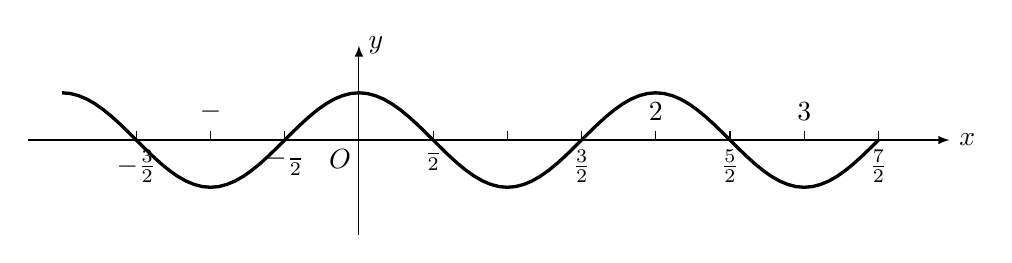
\begin{tikzpicture}[>=latex, scale=.6]
\draw[->] (-7,0)--(12.5,0)node[right]{$x$};
\draw[->] (0,-2)--(0,2)node[right]{$y$};
\foreach \x/\xtext in {-3/-\frac{3\uppi}{2},-1/-\frac{\uppi}{2},1/\frac{\uppi}{2},3/\frac{3\uppi}{2},5/\frac{5\uppi}{2},7/\frac{7\uppi}{2}}
{
    \draw(\x*pi/2, 0)node[below]{$\xtext$}--(\x*pi/2,.2);
}
\foreach \x/\xtext in {-1/-\uppi, 1/\uppi, 2/2\uppi, 3/3\uppi}
{
    \draw(\x*pi, 0)--(\x*pi,.2)node[above]{$\xtext$};
}
\draw [domain=-2*pi:3.5*pi, samples=100, very thick]plot(\x, {cos(\x r)});
\node at (-.4,-.4){$O$};
\end{tikzpicture}
    \caption{}
\end{figure}

\begin{Definition}
    函数$y=\cos x$在闭区间$[0,\uppi]$上的反函数叫做\emph{反
余弦函数}或\emph{反余弦},记作
\[x=\arccos y\]
它的定义域是闭区间$[-1,1]$。
\end{Definition}

用几何名词来叙述这个定义,便是(互换字母$x$、$y$的
位置):在闭区间$-1\leqslant x\leqslant 1$上,数$x$的反余弦
$y=\arccos x$
是在闭区间$[0,\uppi]$的一个角或弧,它的余弦值等于$x$, 即
$\cos y=x$。

\begin{example}
    求下列各式的值(口答):
\begin{tasks}(2)
    \task $\arccos\frac{1}{2}$
    \task $\arccos\left(-\frac{1}{2}\right)$
    \task $\arccos1$
    \task $\arccos0$
\end{tasks}
\end{example}

\begin{solution}
\begin{enumerate}
    \item $\arccos\frac{1}{2}=\frac{\uppi}{3}$,因为$\cos\frac{\uppi}{3}=\frac{1}{2}$,而且$0<\frac{\uppi}{3}<\uppi$。
    \item $\arccos\left(-\frac{1}{2}\right)=\frac{2\uppi}{3}$,因为$\cos\frac{2\uppi}{3}=\cos\left(\uppi-\frac{\uppi}{3}\right)=\frac{1}{2}$,而且$0<\frac{2\uppi}{3}<\uppi$。
    \item $\arccos1=0$,因为$\cos 0=1$而且0不出$[0,\uppi]$的界限。
    \item $\arccos0=\frac{\uppi}{2}$,因为$\cos\frac{\uppi}{2}=1$,而且$0<\frac{\uppi}{2}<\uppi$。
\end{enumerate}
\end{solution}

由反余弦函数的定义和反函数的定理得到反余弦的性质
如下:
\begin{enumerate}
\item $\arccos(\cos y)=y,\; 0\leqslant y\leqslant \uppi,\qquad \cos(\arccos x)=x,\; -1\leqslant x\leqslant 1$
\item 函数$f(x)=\arccos x$在闭区间$[-1,1]$上,由$\uppi$下
降到0, 且连续。
\item 我们知道互补的两个角$\alpha$和$\uppi-\alpha$的余弦是相反
数,即
\[\cos(\uppi-\alpha)=-\cos\alpha\]
反之,在区间$[-1,1]$内的相反数的反余弦互为补角,即
\[\arccos(-x)=\uppi-\arccos x,\qquad x\in [-1,1]\]

\item 反余弦函数$y=\arccos x$的图象如图9.6所示。
\begin{figure}[htp]
    \centering
\begin{tikzpicture}[>=latex, scale=1.8]
    \draw[->] (-2,0)--(2,0)node[right]{$x$};
    \draw[->] (0,-.5)--(0,3.5)node[right]{$y$};
\draw[domain=-1:1, samples=1000, very thick] plot(\x, {acos(\x)*pi/180});
\node at (.1,-.1){$O$};
\foreach \x/\xtext in {-1/-1,1/1,-.4/-x,.4/x}
{
    \draw (\x,0)node[below]{$\xtext$}--(\x,.1);
}
\node at (0,.5*pi) [right]{$\frac{\uppi}{2}$};
\node at (-1,pi) [left]{$y=\arccos x$};
\draw[dashed](-1,0)--(-1,pi)--(0,pi)node[right]{$\uppi$};
\draw[dashed](-.4,0)--(-.4,1.98)--(0,1.98)node[right]{$\arccos(-x)$};
\draw[dashed](.4,0)--(.4,1.16)node[right]{$\arccos x$}--(0,1.16);

\end{tikzpicture}
    \caption{}
\end{figure}
\end{enumerate}

\begin{proof}
    因为$0\leqslant \arccos(-x)\leqslant \uppi$, 又$0\leqslant \uppi -\arccos x\leqslant x$
而且
\[\cos(\uppi -\arccos x)=-\cos(\arccos x)=-x\]
由余弦函数在$[0,\uppi]$ 上是单调的,得到
\[\uppi -\arccos x=\arccos (-x)\]
\end{proof}

\begin{example}
    求下列各式的值:
$\arccos\left(-\frac{\sqrt{2}}{2}\right),\qquad \arccos(-0.9695)$
\end{example}


\begin{solution}
\[\arccos\left(-\frac{\sqrt{2}}{2}\right)=\uppi-\arccos\left(\frac{\sqrt{2}}{2}\right)=\uppi-\frac{\uppi}{4}=\frac{3\uppi}{4}\]
\[\begin{split}
    \arccos(-0.9695)&=180^{\circ}-\arccos0.9695\\
    &=180^{\circ}-14^{\circ}11'=165^{\circ}49'\approx 165.82^{\circ}\\
    &\approx 0.9212\uppi\approx 2.894\text{弧度}
\end{split}\]
\end{solution}


\begin{example}
求$\tan\left[\arccos\left(-\frac{2\sqrt{2}}{3}\right)\right]$的值。
\end{example}

\begin{solution}
设$\arccos\left(-\frac{2\sqrt{2}}{3}\right)=\alpha$,其中$0\leqslant \alpha\leqslant \uppi$,那么,$\cos\alpha=-\frac{2\sqrt{2}}{3}$,由于$0\le\alpha\leqslant \uppi$和$\cos\alpha<0$。可以知道$\alpha$是第二象限的角,所以
\[\tan\alpha=-\sqrt{\frac{1}{\cos^2\alpha}-1}=-\sqrt{\frac{9}{8}-1}=-\sqrt{\frac{1}{8}}=-\frac{\sqrt{2}}{4}\]
\end{solution}


\begin{example}
证明:若$|x|\leqslant 1$,则$\arcsin x+\arccos x=\frac{\uppi}{2}$

\end{example}

\begin{proof}
 $\because\quad    \sin\left(\frac{\uppi}{2}-\arccos x\right)=\cos(\arccos x)=x$

    又    $\sin(\arcsin x)=x$, 且
  \[  0\leqslant \arccos x\leqslant \uppi,\qquad -\frac{\uppi}{2}\leqslant \frac{\uppi}{2}-\arccos x\leqslant \frac{\uppi}{2}\]

$\therefore\quad \arcsin x$和$\frac{\uppi}{2}-\arccos x$是$\sin x$在单调区间$\left[-\frac{\uppi}{2},\frac{\uppi}{2}\right]$上的角。

根据$\sin x$在这区间上的单调性,有
$\arcsin x=\frac{\uppi}{2}-\arccos x$
即:
\[\arcsin x+\arccos x=\frac{\uppi}{2}\]
\end{proof}

\begin{example}
证明:$\arcsin\frac{4}{5}+\arccos\frac{12}{13}+\arcsin\frac{16}{65}=\frac{\uppi}{2}$
\end{example}

\begin{proof}
\[\begin{split}
    \arcsin\frac{4}{5}+\arccos\frac{12}{13}&=\frac{\uppi}{2}-\arcsin\frac{16}{65}\\
&=\arccos\frac{16}{65}
\end{split}\]
    
令$\alpha=\arcsin\frac{4}{5}$,则$\sin\alpha=\frac{4}{5}$,$0<\alpha<\frac{\uppi}{2}$,$\cos\alpha=\frac{3}{5}$。

令$\beta=\arccos\frac{12}{13}$,则$\cos\beta=\frac{12}{13}$,$0<\beta<\frac{\uppi}{2}$,$\sin\beta=\frac{5}{13}$。

因此:\[\begin{split}
    \cos(\alpha+\beta)&=\cos\alpha\cos\beta-\sin\alpha\sin\beta\\
    &=\frac{3}{5}\cdot \frac{12}{13}-\frac{4}{5}\cdot \frac{5}{13}=\frac{16}{65}
\end{split}\]

$\because\quad 0<\alpha+\beta<\uppi$, $\therefore\quad \alpha+\beta=\arccos\frac{16}{65}$,即:
\[\arcsin\frac{4}{5}+\arccos\frac{12}{13}=\arccos\frac{16}{65}=\frac{\uppi}{2}-\arcsin\frac{16}{65}\]

\[\therefore\quad \arcsin\frac{4}{5}+\arccos\frac{12}{13}+\arcsin\frac{16}{65}=\frac{\uppi}{2}\]
\end{proof}

在余弦函数的其它单调区间内,其反函数可按下列方式
去找:

\begin{blk}{命题1}
\begin{enumerate}
    \item 在闭区间$[2k\uppi ,(2k+1)\uppi]$ 上,$y=\cos x$由
    1下降到$-1$, 在这些闭区间上的反函数是
 \[   x=\arccos y+2k\uppi \]
    事实上,角$x\in [2k\uppi ,(2k+1)\uppi]$, 而且它的余弦等于$y$。
    \item 在闭区间$[(2k-1)\uppi ,2k\uppi]$ 上,$y=\cos x$的反函数
    是
\[    x=-\arccos y+2k\uppi \]
    证明相仿。
\end{enumerate}
\end{blk}

\begin{example}
    讨论函数$y=\arccos(\cos x)$的图象。
\end{example}

\begin{solution}
因为$\cos x$的周期是$2\uppi$, 函数$\arccos(\cos x)$也是周期函
数,周期是$2\uppi$, 且
\[\cos y=\cos[\arccos(\cos x)]\]
即:
$\cos y=\cos x$, 这里$0\leqslant y\leqslant \uppi$, $x\in\mathbb{R}$根据上面的命题,
知道:
\begin{enumerate}
    \item 当$x\in[2k\uppi ,(2k+1)\uppi]$ 时,$x=y+2k\uppi$, 即
$y=x-2k\uppi$;
\item  当$x\in[(2k-1)\uppi ,2k\uppi]$ 时,$x=-y+2k\uppi$, 即
$y=-x+2k\uppi$。
\end{enumerate}
函数$y=\arccos(\cos x)$的图象是折线(图5.7)。

\begin{figure}[htp]
    \centering
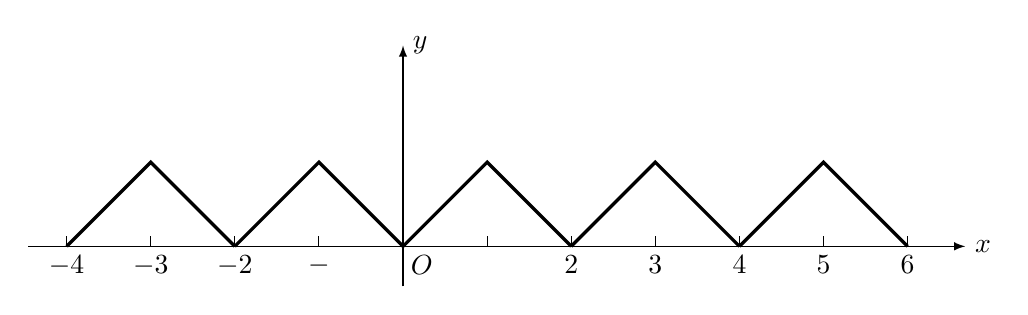
\begin{tikzpicture}[>=latex, scale=.34]
    \draw[->] (-14,0)--(21,0)node[right]{$x$};
    \draw[->] (0,-1.5)--(0,7.5)node[right]{$y$};
\foreach \x in {-4,-2,...,4}
{
    \draw[very thick] (\x*pi,0)--(\x*pi+pi,pi)--(\x*pi+pi+pi,0);
}
\foreach \x in {-4,-3,-2,2,3,4,5,6}
{
    \draw (\x*pi,0)node[below]{$\x\uppi$}--(\x*pi,.4);
}
\foreach \x/\xtext in {-1/-\uppi,1/\uppi}
{
    \draw (\x*pi,0)node[below]{$\xtext $}--(\x*pi,.4);
}
\node at (.7,-.7){$O$};


\end{tikzpicture}    
    \caption{}
\end{figure}
\end{solution}


\begin{Exercise}
\begin{question}
    \item 用反余弦的形式表示下列各式的角($x\in[0,\uppi]$)。
\begin{tasks}(2)
    \task $\cos\uppi =1$
    \task $\cos\frac{5\uppi}{3}=-\frac{1}{2}$
    \task $\cos(-3)=-0.9900$
    \task $\cos\frac{7\uppi}{6}=-\frac{\sqrt{3}}{2}$
    \task $\cos x=-0.8065$
    \task $\cos x=-1$
\end{tasks}

\item 决定下面差的符号:
\begin{tasks}(2)
  \task $\arccos0.7-\arccos0.5$
  \task $\arccos\left(-\frac{3}{5}\right)-\arccos\left(-\frac{3}{4}\right)$
  \task $\arccos\left(\sin\frac{\uppi}{12}\right)-\arccos\left(\sin\frac{\uppi}{13}\right)$
\end{tasks}
\item 不作计算,确定下列各比的符号:
\begin{tasks}(2)
    \task $\frac{\arcsin0.85-\arcsin0.8}{\arccos0.85-\arccos0.8}$
    \task $\frac{\uppi -2\arcsin(0.9)}{\uppi -2\arccos(0.1)}$
    \task $\frac{\arcsin(0.4)+\frac{\uppi}{6}}{\arcsin(0.6)-\frac{\uppi}{3}}$
\end{tasks}

\item 在同一个坐标系中,作函数$y=\arccos x$
和函数$y=\arccos\frac{x}{2}$
的图象,试根据函数图象说明当$x$为何值时,函数
的差$\arccos\frac{x}{2}-\arccos x$
取最大值、最小值、等于零。
\item 计算下列各式的值:
    \begin{tasks}(2)
\task $\sin \left(\arccos \frac{1}{2}\right)$
\task $\sin \left(\arccos \frac{3}{5}\right)$
\task $\tan \left(\arccos \frac{5}{13}\right)$
\task $\arcsin (\cos 1)$
\task $\arccos (\cos 2 \uppi)$
\task $\arccos \left(-\cos \frac{36}{7} \uppi\right)$
\task $\sin \left(\frac{1}{2} \arccos \frac{1}{2}\right)$
\task $\sin \left[3 \arccos \left(-\frac{\sqrt{3}}{2}\right)\right]$
\task $\sin \left[2 \arccos \left(-\frac{2 \sqrt{2}}{3}\right)\right]$
\task $\cos \left(\arcsin \frac{3}{5}-\arccos \frac{5}{13}\right)$    
\task $\sin\left[2\left(\arcsin\frac{\sqrt{5}}{3}-\arccos\frac{\sqrt{5}}{3}\right)\right]$
    \item $\tan\left(\arcsin\frac{1}{2}+\arccos\frac{\sqrt{3}}{2}\right)$
    \end{tasks}

\item 证明下面的恒等式:
\begin{enumerate}
\item 若$0<x<1$, 则:
$\arcsin x=\arccos\sqrt{1-x^2}$
\item 若$0<x<1$, 则:
$\arccos x=\arcsin\sqrt{1-x^2}$
\item 若$-1\leqslant x\leqslant 0$, 则:
$\arcsin x=-\arccos\sqrt{1-x^2}$
\item 若$-1\leqslant x\leqslant 0$, 则:
$\arccos x=\uppi-\arcsin\sqrt{1-x^2}$
\end{enumerate}

\item 解下面的方程:
    \begin{enumerate}
\item $\arccos x=\frac{\uppi}{3}$
\item $\arccos 2x=0.5$
\item $\arcsin x=\arccos x,\; |x|\leqslant 1$
\item $\arcsin x+\arcsin (1-x)=\arccos x$
\item $\arcsin x-\arccos x=\arcsin (3x-2)$
    \end{enumerate}

\item 当$-\frac{1}{2}\leqslant x\leqslant 0$时,求$f(x)
=\arccos x+x^2$的最小值。
\end{question}
\end{Exercise}

\section{反正切函数}

由正切函数$y=\tan x$的图象(图9.8)可以看出,函数$\tan x$
在每个开区间$\left(-\frac{\uppi}{2}+2k\uppi, \frac{\uppi}{2}+2k\uppi\right)$内,由$-\infty$上升到$+\infty$。
所以在每个这样的开区间里能带来一个反函数。


\begin{figure}[htp]
    \centering
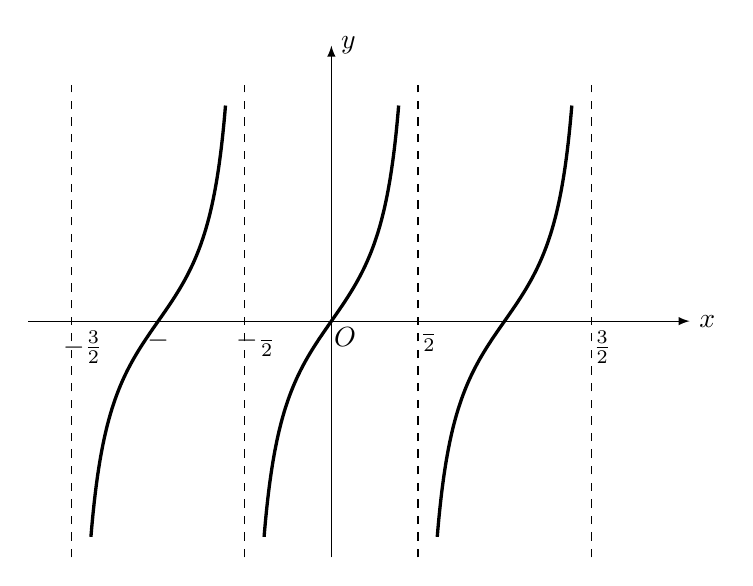
\begin{tikzpicture}[>=latex, xscale=.7]
    \draw[->] (-5.5,0)--(6.5,0)node[right]{$x$};
\draw[->] (0,-3)--(0,3.5)node[right]{$y$};
\foreach \x in {-.5,.5,1.5,-1.5}
{
    \draw[dashed] (\x*pi,-3)--(\x*pi,3);
}

\foreach \y in {-.5,.5,-1.5}
{
    \draw [domain=\y*pi+.35:(\y+1)*pi-.35, samples=1000, very thick] plot(\x, {tan(\x r)});
}

\node at (.25,-.2){$O$};
\node at (-pi,0)[below]{$-\uppi$};
\node at (pi,0)[above]{$\uppi$};

\node at (-.5*pi+.2,0)[below]{$-\frac{\uppi}{2}$};
\node at (.5*pi+.2,0)[below]{$\frac{\uppi}{2}$};
\node at (1.5*pi+.2,0)[below]{$\frac{3\uppi}{2}$};
\node at (-1.5*pi+.2,0)[below]{$-\frac{3\uppi}{2}$};
\end{tikzpicture}
    \caption{}

\end{figure}



\begin{blk}{定义3}
    函数$y=\tan x$在开区间$-\frac{\uppi}{2}<x<\frac{\uppi}{2}$
内的反函数叫做反正切函数 或 反正
切,记作
\[x=\arctan y\]
因为任何实数都可以作为正
切的值,所以反正切定义域是开区间$-\infty<y<+\infty$
\end{blk}

用几何名词来叙述反正
切的定义就是:在开区间
$(-\infty, +\infty)$内,数$y$的反
正切$x=\arctan y$是在开区间$-\frac{\uppi}{2}<x<\frac{\uppi}{2}$
内的一个角或弧,它的正切等于$y$,即:$\tan x=y$。

由定义和反函数定理直接得到反正切的性质如下:
\begin{enumerate}
    \item $\arctan (\tan x)=x, \qquad -\frac{\uppi}{2}<x<\frac{\uppi}{2}$
    
    $\tan (\arctan y)=y,\qquad -\infty<x<+\infty$
    \item $y=\arctan x,\; x\in\mathbb{R}$是单调递增的并且连续;
    \item $\arctan x$是奇函数,即
    \[\arctan (-x)=-\arctan x\]
    证明留给同学们去完成。
    \item 反正切函数$y=\arctan x,\; -\infty<x<+\infty$的图象如
    图5.9所示。
\end{enumerate}

\begin{figure}[htp]
    \centering
\begin{tikzpicture}[>=latex, scale=.7]
    \draw[->] (-5.5,0)--(6.5,0)node[right]{$x$};
    \draw[->] (0,-3)--(0,3)node[right]{$y$};
\draw[dashed] (-5.5,pi/2)--(6.5,pi/2);
\draw[dashed] (-5.5,-pi/2)--(6.5,-pi/2);

\draw [domain=-5.5:5.5, samples=100, very thick]plot(\x, {atan(\x)*pi/180});
\node at (.35,-.35){$O$};
\node at (0,2)[right]{$\frac{\uppi}{2}$};
\node at (0,-2)[right]{$-\frac{\uppi}{2}$};
\node at (5.5,pi/2-.3)[right]{$y=\arctan x$};
\end{tikzpicture}
    \caption{}
\end{figure}



\begin{example}
    求下列各式的值(口答):
\begin{tasks}(2)
    \task $\arctan 1$
    \task $\arctan (-1)$
    \task $\arctan \sqrt{3}$
    \task $\arctan (-\sqrt{3})$
\end{tasks}
\end{example}

\begin{solution}
\begin{enumerate}
    \item $\arctan 1=\frac{\uppi}{4}$,因为$\tan\frac{\uppi}{4}=1$,而且$-\frac{\uppi}{2}<\frac{\uppi}{4}<\frac{\uppi}{2}$
    \item $\arctan (-1)=-\frac{\uppi}{4}$,因为$\tan\left(-\frac{\uppi}{4}\right)=-1$,而且$-\frac{\uppi}{2}<-\frac{\uppi}{4}<\frac{\uppi}{2}$
    \item $\arctan \sqrt{3}=\frac{\uppi}{3}$,因为$\tan\frac{\uppi}{3}=\sqrt{3}$,而且$-\frac{\uppi}{2}<\frac{\uppi}{3}<\frac{\uppi}{2}$
    \item $\arctan (-\sqrt{3})=-\frac{\uppi}{3}$,因为$\tan\left(-\frac{\uppi}{3}\right)=-\sqrt{3}$,而且$-\frac{\uppi}{2}<-\frac{\uppi}{3}<\frac{\uppi}{2}$
\end{enumerate}
\end{solution}

\begin{example}
    求$\cos\left[\arctan\left(-\frac{3}{4}\right)\right]$
\end{example}

\begin{solution}
设$\alpha=\arctan\left(-\frac{3}{4}\right)$,其中$-\frac{\uppi}{2}<\alpha<\frac{\uppi}{2}$,则$\tan\alpha=-\frac{3}{4}$。

由于$-\frac{\uppi}{2}<\alpha<\frac{\uppi}{2}$和$\tan\alpha<0$,可以知道$\alpha$是第四象限的角。所以
\[\begin{split}
    \sec\alpha&=\sqrt{1+\tan^2\alpha}=\sqrt{1+\frac{9}{16}}=\frac{5}{4}\\
    \cos\alpha&=\frac{4}{5}
\end{split}\]
就是
\[\cos\left[\arctan\left(-\frac{3}{4}\right)\right]=\cos\alpha=\frac{4}{5}\]
\end{solution}

关于$y=\tan x$在其它单调区间内的反函数,请看下面命题。

\begin{blk}{命题}
    在开区间$\left(-\frac{\uppi}{2}+k\uppi ,\frac{\uppi}{2}+k\uppi 
\right)$,$k\in\mathbb{Z}$内$y=\tan x$
由$-\infty$上升到$+\infty$, 在这些区间上的反函数是
$x=\arctan y+k\uppi$。
\end{blk}

事实上,$x\in \left(-\frac{\uppi}{2}+k\uppi ,\frac{\uppi}{2}+k\uppi 
\right)$而
且
\[\tan x=\tan (\arctan y+k\uppi )=\tan (\arctan y)=y\]




\begin{example}
    求$\arctan 2+\arctan 3$的值。
\end{example}

\begin{solution}
    $\because\quad \frac{\uppi}{4}=\arctan 1<\arctan 2<\frac{\uppi}{2}$,$\frac{\uppi}{4}=\arctan 1<\arctan 3<\frac{\uppi}{2}$,

    $\therefore\quad \frac{\uppi}{2}<\arctan 2+\arctan 3<\uppi$。而且
\[\begin{split}
    \tan(\arctan 2+\arctan 3)&=\frac{\tan (\arctan 2)+\tan (\arctan  3)}{1-\tan(\arctan 2)\cdot \tan (\arctan 3)}\\
    &=\frac{2+3}{1-2\times 3}=-1
\end{split}\]
由于$\arctan (-1)\in \left(-\frac{\uppi}{2},0\right)$,于是
\[\arctan 2+\arctan 3=\arctan (-1)+\uppi=-\frac{\uppi}{4}+\uppi=\frac{3\uppi}{4}\]
\end{solution}

\begin{example}
    讨论 $y=\arctan (\tan x)$的图象。
\end{example}

\begin{solution}
函数$\arctan (\tan x)$的定义域是除去$x=\frac{\uppi}{2}+k\uppi,\; k\in\mathbb{Z}$
的实数集$\mathbb{R}$, 也就是无数个开区间$\left(-\frac{\uppi}{2}+k\uppi,\frac{\uppi}{2}+k\uppi\right),\; k\in\mathbb{Z}$
所组成的一个并集。因此函数$y=\arctan (\tan x)$的图象在
$x=\frac{\uppi}{2}+k\uppi,\; k\in\mathbb{Z}$这些点处间断。由于
\[\tan y=\tan[\arctan(\tan x)]\]
即:
$\tan y=\tan x$, 这里$-\frac{\uppi}{2}<y<\frac{\uppi}{2}$, $x\ne \frac{\uppi}{2}+k\uppi$。

所以,当$x\in\left(-\frac{\uppi}{2}+k\uppi,\frac{\uppi}{2}+k\uppi\right)$时,$x=y+k\uppi$, 也就是$y=x-k\uppi$。于是:
\begin{itemize}
    \item 当$x\in\left(-\frac{\uppi}{2},\frac{\uppi}{2}\right)$时,$y=x$;
    \item 当$x\in\left(\frac{\uppi}{2},\frac{3\uppi}{2}\right)$时,$y=x-\uppi$;
    \item 当$x\in\left(\frac{3\uppi}{2},\frac{5\uppi}{2}\right)$时,$y=x-2\uppi$;
    \item ………………
    \item 当$x\in\left(-\frac{3\uppi}{2},-\frac{\uppi}{2}\right)$时,$y=x+\uppi$;
    \item ………………
\end{itemize}
现在考虑间断点的情形:

当$\frac{\uppi}{2}+(k-)\uppi<x<\frac{\uppi}{2}+k\uppi$时,$y=x-k\uppi$, 于是当$x$
取每一个数列$\{x_n\}$从左边趋近$\frac{\uppi}{2}+k\uppi$ 时,记作
$x_n\to \left(\frac{\uppi}{2}+k\uppi \right)^-$, 
便有
\[\lim_{x_n\to \left(\tfrac{\uppi}{2}+k\uppi \right)^-}y=\lim_{x_n\to \left(\tfrac{\uppi}{2}+k\uppi \right)^-}(x_n-k\uppi)=\frac{\uppi}{2}+k\uppi-k\uppi=\frac{\uppi}{2}\]

当 $\dfrac{\uppi}{2}+k\uppi <x<\dfrac{\uppi}{2}+(k+1)\uppi$ 时,$y=x-(k+1)\uppi$。于
是当 $x$ 取每一个数列 $\{x_n\}$从右边趋近 $\dfrac{\uppi}{2}+k\uppi$ 时,记作 $x_n\to \left(\frac{\uppi}{2}+k\uppi\right)^+$,便有
\[\lim_{x_n\to \left(\tfrac{\uppi}{2}+k\uppi \right)^+}y=\lim_{x_n\to \left(\tfrac{\uppi}{2}+k\uppi \right)^+}[x_n-(k+1)\uppi]=\frac{\uppi}{2}+k\uppi-k\uppi-\uppi=-\frac{\uppi}{2}\]
因之,函数 $\arctan(\tan x)$ 在间断点$x=\dfrac{\uppi}{2}+k\uppi$ 处的左、右极限存在,其左极限等于 $\dfrac{\uppi}{2}$ 右极限等于 $-\dfrac{\uppi}{2}$,函数图象在这些间断点处,有一个等于 $\uppi$ 的跃度,它的图象如图9.10。

\begin{figure}
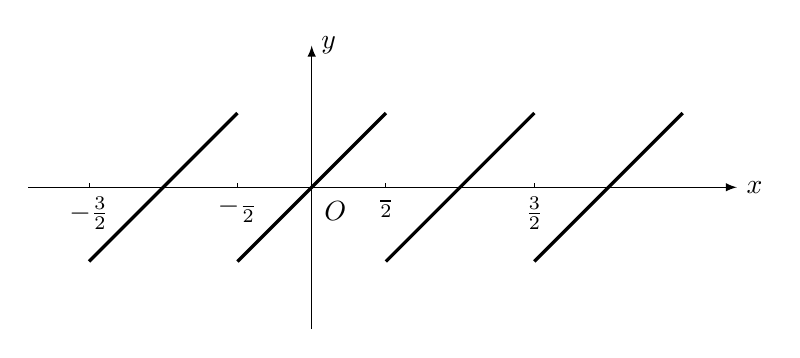
\begin{tikzpicture}[>=latex,scale=.6]
\draw[->] (-6,0)--(9,0)node[right]{$x$};
\draw[->] (0,-3)--(0,3)node[right]{$y$};    
\foreach \x/\xtext in {-1.5*pi/-\frac{3\uppi}{2},-.5*pi/-\frac{\uppi}{2},.5*pi/\frac{\uppi}{2},1.5*pi/\frac{3\uppi}{2}}
{
    \draw (\x,0)node[below]{$\xtext$}--(\x,.1);
}
\foreach \x in {-1.5*pi,-.5*pi,.5*pi,1.5*pi}
{
    \draw[very thick] (\x,-0.5*pi)--(\x+pi,0.5*pi);
}
\node at (.5,-.5){$O$};
\end{tikzpicture}
    \caption{}
\end{figure}
\end{solution}

\section{反余切函数}
由余切函数 $y=\cot x$ 的图象可以看出函数 $\cot x$ 在每个开区
间 $(k\uppi ,(k+1)\uppi ),\; k\in\mathbb{Z}$ 内,由 $+\infty$ 递减到 $-\infty$,所以在每个这样的开区间里,反函数是存在的。

\begin{Definition}
  函数 $y=\cot x$ 在开区间 $(0,\uppi )$ 内的反函数叫\emph{反余切函数或反余切},记作
\[x=\arccot y\]
它的定义域是开区间 $-\infty<y<+\infty$。
\end{Definition}

用几何名词来叙述反余切的定义便是:在开区间 $-\infty<y<+\infty$ 内,数 $y$ 的反余切 $x=\arccot y$ 是开区间 $0<x<\uppi$ 内的一个角或弧,它的余切等于 $y$,即 $\cot x=y$。

由反余切的定义和反函数定理得到反余切的性质如下:
\begin{enumerate}
  \item $\arccot (\cot x)=x,\; 0<x<\uppi ,\qquad \cot (\arccot y)=y,\; -\infty<y<+\infty$
  \item 反余切是递减的函数并且连续;
  \item $\arccot (-x)=\uppi -\arccot x$。

  这是因为$\arccot x$ 和 $\arccot (-x)$ 都属于 $(0,\uppi )$ 内的角,且
  \[0=\uppi -\uppi <\uppi - \arccot x<0+\uppi =\uppi \]
  又 $\cot (\uppi -\arccot x)=-\cot (\arccot x)=-x$,
  所以
  \[\uppi -\arccot x=\arccot (-x)\]
  即
  \[\arccot (-x)=\uppi -\arccot x\]
  \item 反余切 $y=\arccot x,\; -\infty<x<+\infty$ 的图象如\cref{fig:graph_arccot} 所示。
\end{enumerate}

\begin{figure}[htp]
    \centering
\begin{tikzpicture}[>=latex, scale=.8]
\draw[->] (-5,0)--(6,0)node[right]{$x$};
\draw[->] (0,-1)--(0,5)node[right]{$y$};
\draw (-5,pi)--(5,pi);
\node at (.25,-.25){$O$};
\node at (.2,pi)[above]{$\uppi$};
\node at (.2,0.5*pi)[above]{$\frac{\uppi}{2}$};
\draw [domain=.01:5, samples=100, very thick]plot(\x,{atan(1/\x)*pi/180});
\draw [domain=-5:-.01, samples=100, very thick]plot(\x,{atan(1/\x)*pi/180+pi});
\node at (-3.5,2.5){$y=\arccot x$};
\end{tikzpicture}    
    \caption{}\label{fig:graph_arccot}
\end{figure}



\begin{example}
  求下列各式的值:(口答)
  \begin{tasks}(2)
    \task $\arccot 1$
    \task $\arccot (- 1)$
    \task $\arccot \sqrt{3}$
    \task $\arccot \left(-\sqrt{3}\right)$
  \end{tasks}
\end{example}

\begin{solution}
\begin{tasks}
  \task $\arccot 1=\dfrac{\uppi}{4}$,因为 $\cot\dfrac{\uppi}{4}=1$,而且 $0<\dfrac{\uppi}{4}<\uppi$。
  \task $\arccot (- 1)=\uppi-\arccot 1=\uppi-\dfrac{\uppi}{4}=\dfrac{3\uppi}{4}$
  \task $\arccot \sqrt{3}=\dfrac{\uppi}{6}$,因为 $\cot\dfrac{\uppi}{6}=\sqrt{3}$,而且 $0<\dfrac{\uppi}{6}<\uppi$。
  \task $\arccot \left(-\sqrt{3}\right)=\uppi-\arccot\sqrt{3}=\uppi-\dfrac{\uppi}{6}=\dfrac{5\uppi}{6}$
\end{tasks}
\end{solution}

\begin{example}
  求 $\sin\left[\arccot\left(-\dfrac{1}{3}\right)\right]$ 的值
\end{example}

\begin{solution}
  设 $\arccot\left(-\dfrac{1}{3}\right)=\alpha$,其中 $0<\alpha<\uppi$,那么 $\cot\alpha=-\dfrac{1}{3}$。

  由于 $0<\alpha<\uppi$,$\cot\alpha<0$,可以知道 $\dfrac{\uppi}{2}<\alpha<\uppi$
\[\begin{split}
    \csc\alpha&=\sqrt{1+\cot^2\alpha}=\sqrt{1+\frac{1}{9}}=\sqrt{\frac{10}{9}}=\frac{\sqrt{10}}{3}\\
    \sin\alpha&=\frac{1}{\csc\alpha}=\frac{3}{\sqrt{10}}
\end{split}\]
$\therefore\quad \sin\left[\arccot\left(-\dfrac{1}{3}\right)\right]=\sin\alpha=\dfrac{3}{\sqrt{10}}=\dfrac{3\sqrt{10}}{10}$
\end{solution}

\begin{example}
    求证:对于任何实数 $x$ 有
\[\arctan x+\arccot x=\frac{\uppi}{2}\]
\end{example}

\begin{solution}
设 $\arctan x=\alpha$,其中 $-\dfrac{\uppi}{2}<\alpha<\dfrac{\uppi}{2}$,则 $\tan\alpha=x$。

又 $\cot\left(\dfrac{\uppi}{2}-\alpha\right)=\tan\alpha=x$,而 $0<\dfrac{\uppi}{2}-\alpha<\uppi$,所以 $\dfrac{\uppi}{2}-\alpha=\arccot x$。

将 $\alpha=\arctan x$ 代入上式,得到
\[\frac{\uppi}{2}-\arctan x=\arccot x\]
所以:$\arctan x+\arccot x=\dfrac{\uppi}{2},\quad x\in\mathbb{R}$
\end{solution}


\begin{example}
  证明 $\arctan 3+\arccot\left(-\dfrac{1}{5}\right)=\uppi-\arctan\dfrac{1}{8}$
\end{example}

\begin{solution}
设 $\alpha=\arctan 3$,其中 $0<\alpha<\dfrac{\uppi}{2}$,则 $\tan\alpha=3$。

又设 $\beta=\arccot\left(-\dfrac{1}{5}\right)$,其中 $\dfrac{\uppi}{2}<\beta<\uppi$,则:
\[\cot\beta=-\dfrac{1}{5},\qquad \tan\beta=-5\]
\[\begin{split}
 \tan\left[\arctan 3+\arccot\left(-\frac{1}{5}\right)\right]
&=\tan(\alpha+\beta)\\
&=\frac{\tan\alpha+\tan\beta}{1-\tan\alpha\cdot \tan\beta}\\
&=\frac{3+(-5)}{1-3(-5)}=-\frac{1}{8}
\end{split}\]
而且 $\dfrac{\uppi}{2}<\alpha+\beta<\dfrac{3\uppi}{2}$,
\[\therefore\quad \arctan 3+\arccot\left(-\frac{1}{5}\right)=\arctan\left(-\frac{1}{8}\right)+\uppi=\uppi-\arctan\frac{1}{8}\]
\end{solution}

\begin{Exercise}
\begin{question}
  \item 用反三角函数表示下面等式中的角。
  \begin{tasks}(2)
    \task $\displaystyle \tan\left(-\frac{\uppi}{4}\right)=-1$
    \task $\displaystyle \tan\left(\frac{7\uppi}{4}\right)=-1$
    \task $\displaystyle \tan\left(\frac{5\uppi}{6}\right)=-\frac{1}{\sqrt{3}}$
    \task $\displaystyle \tan\left(-\frac{3\uppi}{4}\right)=1$
    \task $\displaystyle \cot\frac{\uppi}{6}=\sqrt{3}$
    \task $\displaystyle \cot\left(-\frac{5\uppi}{4}\right)=-1$
    \task $\displaystyle \cot\left(-1\right)=-0.6421$
  \end{tasks}
  \item 指出下列各函数哪些是偶函数?哪些是奇函数?哪些既不是奇函数也不是偶函数。
  \begin{tasks}(2)
    \task $y=\arcsin x+2 \arctan x$
    \task $y=\arccos x+\arctan x$
    \task $y=\dfrac{\arcsin x}{\arccos x}$
    \task $y=\dfrac{\arctan x}{x}-x \arcsin x$
  \end{tasks}
  \item 计算下列各式的值:
  \begin{tasks}(2)
    \task  $\displaystyle \cos [\arctan(-\sqrt{3})]$;
    \task  $\displaystyle \sin (\arctan 2)$;
    \task  $\displaystyle \arctan(\tan2)$
    \task  $\displaystyle \arctan(\tan0.7 \uppi)$
    \task  $\displaystyle \tan\left(\arctan \frac{1}{4}-\arccot  5\right)$
    \task  $\displaystyle \sin \left(\arctan \frac{8}{15}-\arcsin \frac{7}{18}\right)$
    \task  $\displaystyle \tan\left[2 \arctan\left(-\frac{1}{2}\right)\right]$
    \task  $\displaystyle \cos \left[2 \arctan \frac{1}{4}+\arccos \frac{3}{5}\right]$
  \end{tasks}
  \item 检验下列各等式是否正确。
  \begin{tasks}(2)
    \task $\displaystyle \arcsin \frac{15}{17}=\arccos \frac{8}{17}$
    \task $\displaystyle \arcsin \frac{4}{5}=\arccot\frac{3}{4}$
    \task $\displaystyle \arcsin \left(-\frac{7}{25}\right)=-\arctan \frac{7}{24}$
    \task $\displaystyle \arccos \left(-\frac{9}{41}\right)=\uppi-\arcsin \frac{40}{41}$
    \task $\displaystyle \arctan \frac{2}{3}+\arctan \frac{1}{5}=\frac{\uppi}{4}$
    \task $\displaystyle \arccot\frac{1}{9}+\arccot\frac{4}{5}=\frac{3}{4} \uppi$
    \task! $\displaystyle 2 \arctan \frac{1}{3}+\arctan \frac{1}{4}=\arctan \frac{16}{13}$
    \task! $\displaystyle \arcsin \frac{7}{25}+\frac{1}{2} \arccos \frac{7}{25}=\arccos \frac{3}{5}$
  \end{tasks}   
  \item 证明下面恒等式:
  \begin{question}[label=\alph*),listparindent=0pt]
    \item 若 $0<x<1$, 那么
    \[\arcsin x=\arccos\sqrt{1-x^2}=\arctan\frac{x}{\sqrt{1-x^2}}=\arccot\frac{\sqrt{1-x^2}}{x}\]
    \item 若 $0<x<1$, 那么
    \[\arccos x=\arcsin\sqrt{1-x^2}=\arctan\frac{\sqrt{1-x^2}}{x}=\arccot\frac{x}{\sqrt{1-x^2}}\]
    \item 若 $x>0$, 那么
    \[\arctan x=\arccot \frac{1}{x}=\arcsin\frac{x}{\sqrt{1+x^2}}=\arccos\frac{1}{\sqrt{1+x^2}}\]
    \item 若 $x>0$, 那么
    \[\arccot x=\arctan \frac{1}{x}=\arcsin\frac{1}{\sqrt{1+x^2}}=\arccos\frac{x}{\sqrt{1+x^2}}\]
    \item 若 $|x|\leqslant 1$,那么 $\arcsin x=\arctan\dfrac{x}{\sqrt{1-x^2}}$

    若 $-1\leqslant x\leqslant 0$,那么 $\arcsin x=-\arccos{\sqrt{1-x^2}}$

    若 $-1\leqslant x< 0$,那么 $\arcsin x=\arctan\dfrac{\sqrt{1-x^2}}{x}-\uppi$

    \item 若 $-1\leqslant x\leqslant 0$,那么 $\arccos x=\uppi-\arcsin{\sqrt{1-x^2}}$

    若 $-1\leqslant x< 0$,那么 $\arccos x=\uppi+\arctan\dfrac{\sqrt{1-x^2}}{x}$

    若 $|x|\leqslant 1$,那么 $\arccos x=\arctan\dfrac{x}{\sqrt{1-x^2}}$

    \item 若 $x<0$, 那么 $\arctan x=\arccot \dfrac{1}{x}-\uppi$

    若 $x<0$, 那么 $\arccot x=\uppi+\arctan\dfrac{1}{x}$

    \item 若 $x\geqslant 0$,$\dfrac{1}{2}\arccos(2x^2-1)=\arccos x$
    \item 若 $x\geqslant 1$,$2\arctan x+\arcsin\dfrac{2x}{1+x^2}=\uppi$
  \end{question}
  \item 作函数$y=x-\arctan(\tan x)$的草图。
  \item 解下列方程:
  \begin{tasks}(2)
    \task $\displaystyle \arctan x=\frac{\uppi}{4}$
    \task $\displaystyle \arctan x=\frac{\uppi}{2}$
    \task $\displaystyle \arctan x=-\frac{\uppi}{2}$
    \task $\displaystyle \arctan x^2=3$
    \task $\displaystyle \arctan 2x+\arctan 3x=\frac{3\uppi}{4}$
    \task! $\sin\Big\{2\arccos\big[\cot(2\arctan x)\big]\Big\}=0$
  \end{tasks}
  \item 若 $\arctan x+\arctan y+ \arctan z=\uppi$,求证:$x+y+z=xyz$。
  \item 求证:
  \[\arctan x+\arctan\frac{1-x}{1+x}=\begin{cases}
    \dfrac{\uppi}{4},& x>-1\\
    -\dfrac{3\uppi}{4},& x<-1
  \end{cases}\]
\end{question}
\end{Exercise}

\section{最简单的三角方程}
下列方程 $\sin x=a$,$\cos x=a$,$\tan x=a$,$\cot x=a$ 中的 $a$ 为已给的实数,$x$ 是未知数,是最简单的三角方程。适合其中某
个方程的 $x$ 值叫做这个方程的解或根。例如,诸角:$x=\ang{30}$;$x=\ang{150}$;$x=\ang{390}$;$x=\ang{510}$ 等等,为三角方程
$\sin x=\dfrac{1}{2}$ 的解,因为,
\[\sin\ang{30}=\sin\ang{30}=\sin\ang{30}=\sin\ang{30}=\frac{1}{2}\]

解三角方程就是求它的一切解,根据前一节内容知道,已知三角函数值 $a$ 所对应的角的值,如果存在的话,有无穷多个,所以每一个三角方程都有无穷多个解,它的所有解简称为通解。

在本节中,我们来解上面所示的最简单三角方程,从以后的例子即将明白,解三角方程归根到底化为解最简单的三角方程。

\subsection{最简单三角方程的解}
\subsubsection{$\sin x=a$ 的解}
分 $|a|\leqslant 1$ 和 $|a|>1$ 的情形来考虑:

\textbf{第一种情形:} $0<a<1$
 
在坐标系 $x$-$O$-$y$ 中,以原点 $O$ 为圆心作一单位圆,在 $Oy$ 轴上作出纵坐标等于 $a$ 的 $Q$ 点,并过 $Q$ 点引平行于 $Ox$ 轴的直线,交单位圆周于 $A$和$B$二点,如图9.12, $P_0$为$(1,0)$,
$\angle P_0OA=\arcsin a$和$\angle P_0OB=\uppi-\arcsin a$的正弦都等于$a$,
所以$\arcsin a$ 和$\uppi-\arcsin a$是方程$\sin x=a$的特解,为求方程
$\sin x=a$的通解,可将$2k\uppi$加于此两角中的每一个而得到,其
中$k\in\mathbb{Z}$。 因此,原方程的通解是
\[\begin{split}
   x_1&=2k\uppi +\arcsin a\\
x_2&=2k\uppi +\uppi -\arcsin a=(2k+1)\uppi -\arcsin a 
\end{split}\]
合并起来,可写成
\[x=k\uppi +(-1)^k\arcsin a,\qquad k\in\mathbb{Z}\]

我们约定,在三角方程的通解中,“$k\in\mathbb{Z}$”以后不再
交代。

\begin{figure}[htp]\centering
    \begin{minipage}[t]{0.48\textwidth}
    \centering
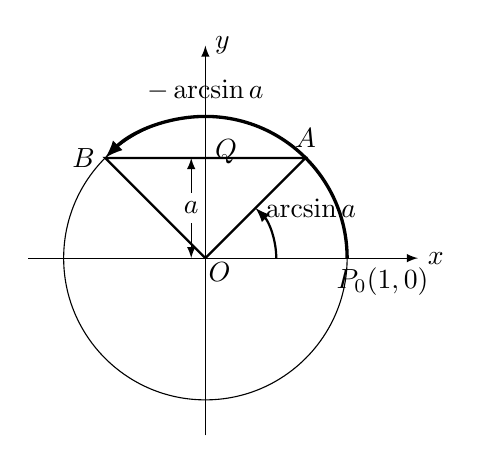
\begin{tikzpicture}[>=latex, scale=.9]
\draw [<->](-.2,0)--node[fill=white]{$a$}(-.2,1.414);
\draw[->] (-2.5,0)--(3,0)node[right]{$x$};
\draw[->] (0,-2.5)--(0,3)node[right]{$y$};
\draw (0,0) circle (2);
\draw[thick] (0,0)--(45:2)node[above]{$A$}--(135:2)node[left]{$B$}--(0,0);
\node at (.2,-.2){$O$};
\node at (0,1.5)[right]{$Q$};
\node at (2.5,0)[below]{$P_0(1,0)$};
\draw[->,  thick] (1,0) arc (0:45:1)node[right]{$\arcsin a$};
\draw[->, very thick] (2,0) arc (0:135:2);
\node at (0,2)[above=2pt]{$\uppi-\arcsin a$};
    \end{tikzpicture}
    \caption{}
    \end{minipage}
    \begin{minipage}[t]{0.48\textwidth}
    \centering
    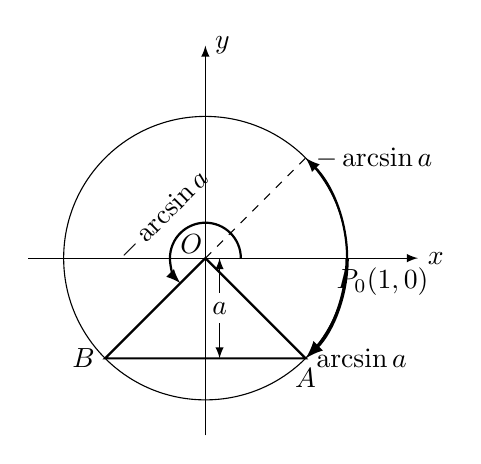
\begin{tikzpicture}[>=latex, scale=.9]
\draw [<->](.2,0)--node[fill=white]{$a$}(.2,-1.414);
\draw[->] (-2.5,0)--(3,0)node[right]{$x$};
\draw[->] (0,-2.5)--(0,3)node[right]{$y$};
\draw (0,0) circle (2);
\node at (-.2,.2){$O$};
\node at (2.5,0)[below]{$P_0(1,0)$};
\draw[thick] (0,0)--(-45:2)node[below]{$A$}--(-135:2)node[left]{$B$}--(0,0);
\draw[dashed] (0,0)--(45:2);
\draw[->, thick] (2,0) arc (0:45:2)node[right]{$-\arcsin a$};
\draw[->, very thick] (2,0) arc (0:-45:2)node[right]{$\arcsin a$};
\draw[->, thick] (.5,0) arc (0:180+45:.5);
\node at (-.6,.6)[rotate=45]{$\uppi-\arcsin a$};

    \end{tikzpicture}
    \caption{}
    \end{minipage}
    \end{figure}


\emph{第二种情形:} $-1<a<0$

用同样的方法作图,如图9.13所示:
$\angle P_0OA=\arcsin a$和$\angle P_0OB=\uppi-\arcsin a$是方程$\sin x=a,\; -1<a<0$的特解,因此,原方程的通解仍是
\[\begin{split}
  x_1&=2k\uppi +\arcsin a\\
x_2&=2k\uppi +\uppi -\arcsin a=(2k+1)\uppi -\arcsin a  
\end{split}\]
合并起来,可写成
\[x=k\uppi +(-1)^k\arcsin a\]

\emph{第三种情形:} $a=1$

方程$\sin x=1$的特解是$x=\frac{\uppi}{2}$,
因此,原方程的通解是
\[x=\frac{\uppi}{2}+2k\uppi\quad \text{或者}\quad x=90^{\circ}+k\cdot 360^{\circ}\]

\emph{第四种情形:} $a=-1$

\[\sin x=-1\]
特解:$x=-\frac{\uppi}{2}$(或$x=-90^{\circ}$),

通解:$x=-\frac{\uppi}{2}+2k\uppi$ (或$x=-90^{\circ}+k\cdot 360^{\circ}$)。

\emph{第五种情形:} $a=0$

\[\sin x=0\]
特解:$x_1=0$和$x_2=\uppi$。

通解:$x_1=2k\uppi$和$x_2=\uppi +2k\uppi =(2k+1)\uppi$,
合并成:\[x=k\uppi\]

\emph{第六种情形:} $|a|>1$

在这种情形下,$\sin x=a$没有解。

将结果总结于下表内
\begin{center}
\begin{tabular}{c|c}
    \hline
$a$的数值& 方程$\sin x=a$的解\\
    \hline
$-1<a<0,\; 0<a<1$ & $x=k\uppi +(-1)^k\arcsin a$\\
$a=-1$& $x=-\frac{\uppi}{2}+2k\uppi$\\
$a=0$&   $x=k\uppi$\\
$a=1$& $x=\frac{\uppi}{2}+2k\uppi$\\
$|a|>1$ & 方程无解\\
    \hline
\end{tabular}   
\end{center}

\begin{example}
    解方程$\sin x=\frac{1}{2} $
\end{example}

\begin{solution}
    \[x=k\uppi+(-1)^k\arcsin\frac{1}{2}=k\uppi+(-1)^k\frac{\uppi}{6}\]
    或者\[x=k\cdot 360^{\circ}+(-1)^k\cdot 30^{\circ},\qquad (k\in\mathbb{Z})\]
\end{solution}


\begin{example}
    解方程$\sin x=-\frac{1}{2} $
\end{example}

\begin{solution}
\[x=k\uppi+(-1)^k\arcsin\left(-\frac{1}{2}\right)=k\uppi+(-1)^{k+1}\frac{\uppi}{6}\]
    或者\[x=k\cdot 360^{\circ}+(-1)^{k+1}\cdot  30^{\circ},\qquad (k\in\mathbb{Z})\]
\end{solution}


\begin{example}
    解方程$\sin (2x-1)=\frac{\sqrt{3}}{2} $
\end{example}

\begin{solution}
\[\begin{split}
   2x-1&=k\uppi+(-1)^k \arcsin\frac{\sqrt{3}}{2}\\ 
2x&=k\uppi+(-1)^k \cdot \frac{\uppi}{3}+1\\
  x &=k\cdot\frac{\uppi}{2}+(-1)^k\cdot \frac{\uppi}{6}+\frac{1}{2} ,\qquad (k\in\mathbb{Z})
 \end{split}\]   
\end{solution}

\subsubsection{$\cos x=a$的解}

\emph{第一种情形:} $0<a<1$
在$Ox$轴上作出横坐标等于$a$的$P$点,并过$P$点作平行于$Oy$
轴的直线交单位圆周于$C$和$D$二点,$P_0$为$(1,0)$(图9.14)。
$\angle P_0OC=\arccos a$和$\angle P_0OD=-\arccos a$的余弦等于$a$, 故它
们是方程的解,原方程的通解是
\[x=2k\uppi\pm \arccos a\]

\emph{第二种情形:} $-1<a<0$
作类似的图形,如图9.15同样可得原方程的通解是
\[x=2k\uppi\pm \arccos a\]

\begin{figure}[htp]\centering
    \begin{minipage}[t]{0.48\textwidth}
    \centering
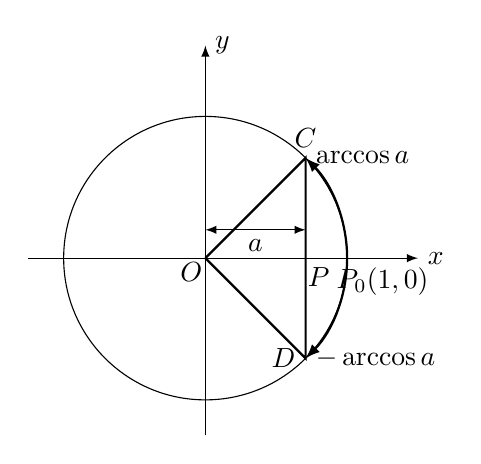
\begin{tikzpicture}[>=latex, scale=.9]
\draw [<->](0,.4)--node[below]{$a$}(1.414,.4);
\draw[->] (-2.5,0)--(3,0)node[right]{$x$};
\draw[->] (0,-2.5)--(0,3)node[right]{$y$};
\draw (0,0) circle (2);
\draw[thick] (0,0)--(45:2)node[above]{$C$}--(-45:2)node[left]{$D$}--(0,0);
\node at (-.2,-.2){$O$};
\node at (1.6,0)[below]{$P$};
\node at (2.5,0)[below]{$P_0(1,0)$};
\draw[->,  thick] (2,0) arc (0:45:2)node[right]{$\arccos a$};
\draw[->,  thick] (2,0) arc (0:-45:2)node[right]{$-\arccos a$};
    \end{tikzpicture}
    \caption{}
    \end{minipage}
    \begin{minipage}[t]{0.48\textwidth}
    \centering
    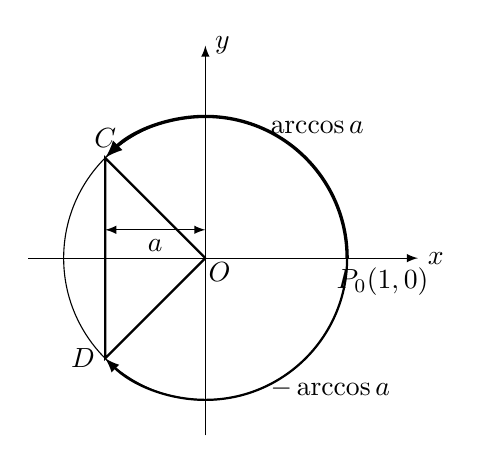
\begin{tikzpicture}[>=latex, scale=.9]
\draw [<->](0,.4)--node[below]{$a$}(-1.414,.4);
\draw[->] (-2.5,0)--(3,0)node[right]{$x$};
\draw[->] (0,-2.5)--(0,3)node[right]{$y$};
\draw (0,0) circle (2);
\draw[thick] (0,0)--(135:2)node[above]{$C$}--(-135:2)node[left]{$D$}--(0,0);
\node at (.2,-.2){$O$};
\node at (2.5,0)[below]{$P_0(1,0)$};
\draw[->, very thick] (2,0) arc (0:135:2);
\draw[->,  thick] (2,0) arc (0:-135:2);
\node at (67:2)[right]{$\arccos a$};
\node at (-67:2)[right]{$-\arccos a$};
    \end{tikzpicture}
    \caption{}
    \end{minipage}
    \end{figure}

\emph{第三种情形:} $a=1$

\[\cos x=1\]

方程的特解:$x=0$, 方程的通解:$x=2k\uppi$。

\emph{第四种情形:} $a=-1$

\[\cos x=-1\]
方程的特解:$x=\uppi$, 方程的通解:$x=\uppi+2k\uppi=(2k+1)\uppi$。

\emph{第五种情形:} $a=0$
\[\cos x=0\]
方程的特解:$x_1=\frac{\uppi}{2}$和$x_2=-\frac{\uppi}{2}=\frac{\uppi}{2}-\uppi$。

方程的通解:$x=\frac{\uppi}{2}+k\uppi$。

\emph{第六种情形:} $|a|>1$

在这种情形下,方程$\cos x=a$无解。

将结果综合于下表内:
\begin{center}
    \begin{tabular}{c|c}
        \hline
    $a$的数值& 方程$\cos x=a$的解\\
        \hline
    $-1<a<0,\; 0<a<1$ & $x=2k\uppi \pm \arccos a$\\
    $a=-1$& $x=(2k+1)\uppi$\\
    $a=0$&   $x=\frac{\uppi}{2}+k\uppi$\\
    $a=1$& $x=2k\uppi$\\
    $|a|>1$ & 方程无解\\
        \hline
    \end{tabular}   
    \end{center}



\begin{example}
    解方程$2\cos x+1=0$
\end{example}

\begin{solution}
    化简为$\cos x=-\frac{1}{2}$,通解如下:
\[\begin{split}
    x&=2k\uppi\pm\arccos\left(-\frac{1}{2}\right)\\
    &=2k\uppi\pm \left(\uppi-\arccos\frac{1}{2}\right)\\
    &=2k\uppi\pm \left(\uppi-\frac{\uppi}{3}\right)\\
    &=2k\uppi\pm \frac{2\uppi}{3}
\end{split}\]
\end{solution}


\begin{example}
    解方程$\cos\left(\frac{x}{4}+\frac{\uppi}{5}\right)=0$
\end{example}

\begin{solution}
    \[\begin{split}
        \frac{x}{4}+\frac{\uppi}{5}&=\frac{\uppi}{2}+k\uppi\\
        \frac{x}{4}&=\frac{\uppi}{2}-\frac{\uppi}{5}+k\uppi=\frac{3\uppi}{10}+k\uppi\\
        x&=4\left(\frac{3\uppi}{10}+k\uppi\right)=\frac{6\uppi}{5}+4k\uppi
    \end{split}
    \]
\end{solution}

\subsubsection{$\tan x=a$的解}

如图9.16所示,$\angle P_0OA=\arctan a$和$\angle P_0OB=\uppi+\arctan a$
是方程的解,因为它们的正切等于 $a$。原方程的通解是
\[x=k\uppi+\arctan a\]


\begin{example}
    解方程$\tan x=-1$    
\end{example}

\begin{solution}
\[x=k\uppi+\arctan(-1)=k\uppi-\arctan1=k\uppi-\frac{\uppi}{4}\]
\end{solution}

\subsubsection{$\cot x=a$的解}

如图9.17所示,$\angle P_0OA=\arccot a$ 和 $\angle P_0OB=\uppi+\arccot a$ 是方
程的特解,因为它们的余切等于$a$。原方程的通解是
\[x=k\uppi+\arccot a,\qquad (k\in\mathbb{Z})\]

\begin{figure}[htp]\centering
    \begin{minipage}[t]{0.48\textwidth}
    \centering
\begin{tikzpicture}[>=latex, scale=.9]
\draw [|<->|](2.2,0)--node[right]{$a$}(2.2,2);
\draw[->] (-2.5,0)--(3,0)node[right]{$x$};
\draw[->] (0,-2.5)--(0,3)node[right]{$y$};
\draw (0,0) circle (2);
\draw[thick] (-135:2)node[below]{$B$}--(0,0)--(45:2)node[above]{$A$}--(2,2);
\node at (.2,-.2){$O$};
\node at (2.7,0)[below]{$P_0(1,0)$};
\draw[->, very thick] (2,0) arc (0:45:2);
\draw[->,  thick] (2,0) arc (0:180+45:2);
\node at (1,.3){$\arctan a$};
\node at (-2,1.5){$\uppi+\arctan a$};
\draw(2,-2.5)--(2,3)node[right]{正切线};
    \end{tikzpicture}
    \caption{}
    \end{minipage}
    \begin{minipage}[t]{0.48\textwidth}
    \centering
    \begin{tikzpicture}[>=latex, scale=.9]
\draw [|<->|](0,2.2)--node[above]{$a$}(2,2.2);
\draw[->] (-2.5,0)--(3,0)node[right]{$x$};
\draw[->] (0,-2.5)--(0,3)node[right]{$y$};
\draw (0,0) circle (2);
\draw[thick] (-135:2)node[below]{$B$}--(0,0)--(45:2)node[above]{$A$}--(2,2);
\node at (.2,-.2){$O$};
\node at (2.7,0)[below]{$P_0(1,0)$};
\draw[->, very thick] (2,0) arc (0:45:2);
\draw[->,  thick] (2,0) arc (0:180+45:2);
\node at (23:2.2)[right]{$\arccot a$};
\node at (-2,1.5){$\uppi+\arccot a$};
\draw(-2.5,2)--(3,2)node[above]{余切线};
    \end{tikzpicture}
    \caption{}
    \end{minipage}
    \end{figure}


\begin{example}
    解方程 $9\cot^2 2x-25=0$
\end{example}

\begin{solution}
    \[\begin{split}
        \cot^2 2x&=\frac{25}{9}\\
        \cot 2x&=\pm\frac{5}{3}\approx \pm 1.6667
    \end{split}\]
由$\cot 2x=1.6667$,得:
\[\begin{split}
    2x&=30^{\circ}58'+k\cdot 180^{\circ}\\
    x&=15^{\circ}29'+k\cdot 90^{\circ}
\end{split}\]
由$\cot 2x=-1.6667$,得:
\[\begin{split}
    2x&=(180^{\circ}-30^{\circ}58')+k\cdot 180^{\circ}\\
    2x&=149^{\circ}2'+k\cdot 180^{\circ}\\
    x&=74^{\circ}31'+k\cdot 90^{\circ}
\end{split}\]
$\therefore\quad $原方程的近似解是:
\[x=15^{\circ}29'+k\cdot 90^{\circ}\quad \text{和}\quad x=74^{\circ}31'+k\cdot 90^{\circ}\]
\end{solution}

\subsection{解简单三角方程的例子}
在本节中,我们来研究某些三角方程的解法。解这些方程时,一般是应用三角函数的恒等变形和解代数方程的一般知识把它归结成解一个或几个最简单的三角方程,从而求出所有解。在解三角方程的过程中,应当避免作可能破坏方程同解性的变形,如果这类变形不可避免,则需研究哪些根会失掉,哪些根是增根,对最终方程的诸解,应当进行检验,确定它们是否是原方程的解。下面通过例子来阐明。

\subsubsection{含有同角的同名三角函数的方程}
\begin{example}
  解方程 $2\cos^2x+\cos x-1=0$
\end{example}

\begin{solution}
把方程看作关于未知数为 $\cos x$ 的二次方程,按照二次方程的解法,可得
\[\cos x=\frac{-1\pm\sqrt{1+8}}{4}=\frac{-1\pm 3}{4}\]
由此得:$\cos x=\dfrac{1}{2}$ 或 $\cos x=-1$。

由 $\cos x=\dfrac{1}{2}$,得:$x=2k\uppi+\frac{\uppi}{3}$;由 $\cos x=-1$,得:$x=(2k+1)\uppi$。

$\therefore\quad $ 原方程的解集是
\[\left\{x\big| x=2k\uppi\pm \frac{\uppi}{3}\right\}\cup \left\{x\big| x=(2k+1)\uppi \right\}\]
\end{solution}

\begin{example}
  解方程 $2\sin^2x+2\sin x-\sqrt{3}\sin x=\sqrt{3}$
\end{example}

\begin{solution}
\textbf{解法1:} 把一切项都移至左端,得:$2\sin^2x+\left(2-\sqrt{3}\right)\sin x-\sqrt{3}=0$。解关于 $\sin x$ 的二次方程,得
\[\begin{split}
\sin x&=\frac{-2+\sqrt{3}\pm \sqrt{\left(2-\sqrt{3}\right)^2+8\sqrt{3}}}{4}\\
&=\frac{-2+\sqrt{3}\pm \sqrt{4+4\sqrt{3}+3}}{4}\\
&=\frac{-2+\sqrt{3}\pm \sqrt{\left(2+\sqrt{3}\right)^2}}{4}\\
&=\frac{-2+\sqrt{3}\pm \left(2+\sqrt{3}\right)}{4}
\end{split}\]
由此得
\[\sin x=\frac{\sqrt{3}}{2}\quad \text{或}\quad \sin x=-1\]

由 $\sin x=\dfrac{\sqrt{3}}{2}$ 得:$x=k\cdot \ang{180}+(-1)^k\cdot \ang{60}$。

由 $\sin x=-1$ 得:$x=-\ang{90}+k\cdot \ang{360}$。

$\therefore\quad $ 原方程的解集是
\[\left\{x|x=k\cdot 180^{\circ}+(-1)^k\cdot 60^{\circ}\right\}\cup \left\{x|x=-90^{\circ}+k\cdot 360^{\circ}\right\}\]
这里 $k\in\mathbb{Z}$。

\emph{解法2:} 把一切项都移至左端得:$2\sin^2x+2\sin x-\sqrt{3}\sin x-\sqrt{3}=0$

方程左端可以分解因式:
\[\begin{split}
    2\sin x(\sin x+1)-\sqrt{3}(\sin x+1)&=0\\
    (\sin x+1)\left(2\sin x-\sqrt{3}\right)&=0
\end{split}\]

若两个因式的乘积等于零,则至少有一个因式等于零,同时应当满足下列条件:对于使第一个因式为零的解,应当使方程的第二个因式有确定的值。上面的方程可分为这样的
两个方程:
\[2\sin x-\sqrt{3}=0\quad \text{或}\quad \sin x+1=0\]
分别由$\sin x=\frac{\sqrt{3}}{2} $和$\sin x=-1$,得到:
\[x=k\uppi+(-1)^k \cdot\frac{\uppi}{3}\quad \text{和}\quad x=-\frac{\uppi}{2}+2k\uppi\]

把$x=k\uppi+(-1)^k \cdot\frac{\uppi}{3}$代入$\sin x+1$中,有确定值,同
样把$x=-\frac{\uppi}{2}+2k\uppi$代入$2\sin x-\sqrt{3}$中,也有确定值,所以
原方程的解集是
\[\left\{x\Big|x=k\uppi+(-1)^k \cdot\frac{\uppi}{3}\right\}\bigcup \left\{x\Big|x=-\frac{\uppi}{2}+2k\uppi\right\}\]
\end{solution}

一般的情况下,在三角方程中,不只有一个三角函数,
我们可以利用同一个角的各三角函数值之间的关系式,把方
程中未知角的各三角函数都用某一个三角函数表示出来,这
样,就把所解的三角方程先归结到多项式方程的问题。

\begin{example}
    解方程 $\sin^2 x+\cos x+1=0$
\end{example}

\begin{solution}
$\because\quad \sin^2 x=1-\cos^2x$,\qquad $\therefore\quad $原方程可化为:
\[\begin{split}
    \cos^2x-\cos x-2&=0\\
    \cos x&=\frac{1\pm 3}{2}
\end{split}\]
由此得到
\[\cos x=2\quad \text{或}\quad \cos x=-1\]

$\because\quad \cos x=2>1$,\qquad  $\therefore\quad $方程无解。

由$ \cos x=-1$,得:$x=(2k+1)\uppi$

$\therefore\quad $原方程的解集是$\{x|x=(2k+1)\uppi,\; k\in\mathbb{Z}\}$。
\end{solution}

\begin{example}
    解方程$\cos x-\sin x=0$
\end{example}

\begin{solution}
    如果用$\cos x$表示$\sin x$或用$\sin x$表示$\cos x$, 那么我们就
    得到根式方程,为了避免这点,可以用$\cos x$去除方程的两
    边,得到
    \[1-\tan x=0\]
    因为原方程的解不含有$\cos x=0$的解,所以我们有根据这样
    做。事实上,由$\cos x=0$, 得到
    $x=\frac{\uppi}{2}+k\uppi$, 代入$\cos x-\sin x$中,有
   \[ \cos\left(\frac{\uppi}{2}+k\uppi \right)-sin\left(\frac{\uppi}{2}+k\uppi \right)=0-(-1)^k\sin \frac{\uppi}{2}=(-1)^{k+1}\ne 0\]
    不满足原方程。
    
    因此,用$\cos x$去除原方程的两边,得到和原方程同解的方程
    \[\tan x=1\]
    由此,
   $ x=k\uppi +\frac{\uppi}{4}$。

   所以原方程的解集是
$\left\{x\Big|x=k\uppi+\frac{\uppi}{4},\; k\in\mathbb{Z}\right\}$
\end{solution}

\begin{rmk}
当解$\cos x-\sin x=0$时,也可以把
$\cos x$提出括号之外,而不用$\cos x$去除两端,原方程可写成下面的形式
$$\cos x (1-\tan x)=0$$
由此得到
$$\cos x=0\quad \text{或}\quad \tan x=1$$
但是使$\cos x=0$的解:$x=\frac{\uppi}{2}+k\uppi$却使因式$1-\tan x$无意义,这就表示$x=\frac{\uppi}{2}+k\uppi$是原方程的增根,因此必须舍去,同样我们得到原方程的同解方程
$\tan x=1$。

对于例9.29这种方程的解法还可以应用到下面更一般的类
型上去。

左端是关于$\sin x$和$\cos x$的齐次多项式右端是零的方程,
称为\emph{齐次方程},例9.29的方程是齐次方程的一个特例。
\end{rmk}




\begin{example}
    解齐次方程$2\sin^2x-7\sin x\cos x+6\cos^2x=0$
\end{example}

\begin{solution}
用$\cos^2x$除原方程的两端,得
\[2\tan^2 x-7\tan x+6=0\]
由此得$\tan x=2\quad \text{或}\quad \tan x=1.5$

由$\tan x=2$得
\[x\approx k\cdot 180^{\circ}+63^{\circ}26'\]

由$\tan x=1.5$得
\[x\approx k\cdot 180^{\circ}+56^{\circ}19'\]
$\therefore\quad $原方程的解集是:
\[\left\{x\big|x=k\cdot 180^{\circ}+63^{\circ}26' \right\}\cup \left\{x\big|x=k\cdot 180^{\circ}+56^{\circ}19' \right\}\]
或者
\[\left\{x\big|x=k\uppi+\arctan 2 \right\}\bigcup\left\{x\big|x=k\uppi+\arctan\frac{3}{2} \right\}\]

又这样的方程
$2\sin^2x+5\sin x\cos x+\cos^2x=4$
也可以归入齐次方程,因为原方程可写成
\[2\sin^2x+5\sin x\cos x+\cos^2x-4(\cos^2x+\sin^2x)=0\]
化简得
\[2\sin^2x-5\sin x\cos x+3\cos^2x=0\]
\end{solution}

\begin{example}
    解方程$8\sin^2\frac{x}{2}+3\sin x-4=0$
\end{example}

\begin{solution}
    原方程可以变形为齐次方程
\[8\sin^2\frac{x}{2}+6\sin \frac{x}{2}\cos\frac{x}{2}-4\left(\sin^2\frac{x}{2}+\cos^2\frac{x}{2}\right)=0\]
化简得:$2\sin^2\frac{x}{2}+3\sin\frac{x}{2}\cos\frac{x}{2}-2\cos^2\frac{x}{2}=0$。

两边除以$\cos^2\frac{x}{2}$, 得
    \[2\tan^2\frac{x}{2}+3\tan\frac{x}{2}-2=0\]
所以$\tan\frac{x}{2}=-2\quad \text{或}\quad \tan\frac{x}{2}=\frac{1}{2}$。

由$\tan\frac{x}{2}=-2$得:
\[\begin{split}
    \frac{x}{2}&=-\arctan 2+k\uppi\\
    x=-2\arctan 2+2k\uppi
\end{split}\]

由$\tan\frac{x}{2}=\frac{1}{2}$得:
\[\begin{split}
    \frac{x}{2}&=\arctan \frac{1}{2}+k\uppi\\
    x=2\arctan \frac{1}{2}+2k\uppi
\end{split}\]
因为原方程的解不含有$\cos^2\frac{x}{2}=0$的解,所以,这样解不会
丢根,由此知原方程的解是
\[\left\{x\big|x=-2\arctan 2+2k\uppi \right\}\cup \left\{x\big|x=2\arctan \frac{1}{2}+2k\uppi \right\}\]
\end{solution}

\subsubsection{一边为零,另一边可以分解为因式的乘积的方程}
\begin{example}
    解方程
$1-\cos x =\tan x-\sin x$
\end{example}

\begin{solution}
    原方程可变形为:$1-\cos x =\tan x(1-\cos x)$

    如果方程的两边除以$1-\cos x$, 那么,原方程中就会丢掉$1-\cos x=0$的根。
为了不致丢掉这些根,把因式$1-\cos x$
提出,方程就变
形为:
\[(1-\cos x)(1-\tan x)=0\]
于是
$$1-\cos x=0\quad  \text{或}\quad 1-\tan x=0$$
由$\cos x=1$得到$x=2k\uppi$, 由$\tan x=1$得到$x=\frac{\uppi}{4}+k\uppi$。

由于方程$\cos x=1$的解使因式$1-\tan x$有确定值,而方程
$\tan x=1$的解也使因式$1-\cos x$有确定值,所以原方程的解集是
\[\left\{x\big|x=2k\uppi\right\}\cup \left\{x\big|x=\frac{\uppi}{4}+k\uppi\right\}\]
\end{solution}


\begin{example}
    解方程 $\tan x+\tan 2x-\tan 3x=0$
\end{example}

\begin{solution}
    原方程可写成
    $\tan 3x(1-\tan x\cdot \tan 2x)-\tan 3x=0$

    化简得:$\tan x\cdot \tan 2x\cdot \tan 3x=0$,由此得:
 \[ \tan  x=0 \quad \text{或}\quad \tan 2x=0 \quad \text{或}\quad \tan 3x=0\]
    由$\tan x=0$得$x=k\uppi$;由$\tan 2x=0$得
    $x=\frac{k\uppi}{2}$;由$\tan 3x=0$得$x=\frac{k\uppi}{3}$
 
    把各方程的解标在单位圆上,得到满足各方程的角的终
    边,如图9.18所示。
\begin{figure}[htp]
    \centering
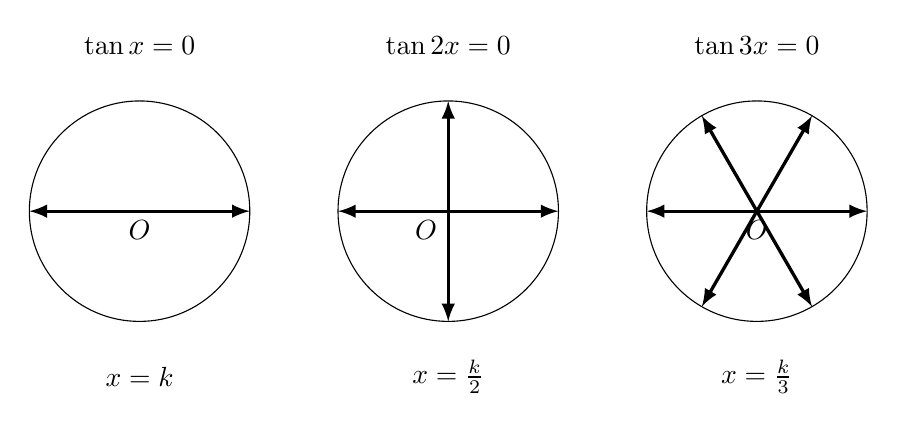
\begin{tikzpicture}[>=latex, scale=1.4]
\begin{scope}
    \draw (0,0) circle (1);
    \draw[<->, very thick] (0:1)--(180:1);
    \node at (0,0)[below]{$O$};
\node at (0,1.5){$\tan x=0$};
\node at (0,-1.5){$x=k\uppi$};
\end{scope}
\begin{scope}[xshift=2.8cm]
    \draw (0,0) circle (1);
    \draw[<->, very thick] (0:1)--(180:1);
    \draw[<->, very thick] (90:1)--(-90:1);
    \node at (-.2,0)[below]{$O$};
\node at (0,1.5){$\tan 2x=0$};
\node at (0,-1.5){$x=\frac{k\uppi}{2}$};
\end{scope}
\begin{scope}[xshift=5.6cm]
    \draw (0,0) circle (1);
    \draw[<->, very thick] (0:1)--(180:1);
    \draw[<->, very thick] (60:1)--(180+60:1);
    \draw[<->, very thick] (120:1)--(-60:1);
    \node at (0,0)[below]{$O$};
\node at (0,1.5){$\tan 3x=0$};
\node at (0,-1.5){$x=\frac{k\uppi}{3}$};
\end{scope}
\end{tikzpicture} 
    \caption{}
\end{figure}

$\because\quad \tan x=0$的解$x=k\uppi=3k\cdot \frac{\uppi}{3}\in \{x|tan 3x=0\}=\left\{x\big| x=k\cdot \frac{\uppi}{3}\right\}$

又$\tan 2x=0$的解$x=k\cdot \frac{\uppi}{2}$
中,当$k=2n+1$时,使$\tan x$没有确定
值,必须舍去;又当$k=2n$时,
\[x=n\uppi=3n\cdot \frac{\uppi}{3}\in\left\{x\big|x=k\cdot \frac{\uppi}{3}\right\}=\{x|\tan 3x=0\}\]
因此,所求方程的解集是
$\left\{x\big|x=k\cdot \frac{\uppi}{3},\quad k\in\mathbb{Z}\right\}$
\end{solution}

\begin{example}
    解方程
$\sin x+\tan x=\sec x-\cos x$
\end{example}

\begin{solution}
两边同乘以$\cos x$, 得到
$\sin x\cos x+\sin x=1-\cos^2x$
移项,提取公因式得
\[\sin x(\cos x +1-\sin x)=0\]
由此得
\[\sin x=0\quad  \text{或}\quad \cos x+1-\sin x=0\]

由 $\sin x=0$, 得 $x=k\uppi$。 

由 $\sin x-\cos x=1$,变形为 $\sin x-\sin(90^{\circ}-x)=1$,即:
\[2\cos45^{\circ} sin\left(x-\frac{\uppi}{4}\right)=1\]
即 $\sin\left(x-\frac{\uppi}{4}\right)=\frac{\sqrt{2}}{2}$

由此得:
\[x-\frac{\uppi}{4}=\frac{\uppi}{4}+2k\uppi\quad  \text{或}\quad x-\frac{\uppi}{4}=\frac{3\uppi}{4}+2k\uppi\]
即
\[x=\frac{\uppi}{2}+2k\uppi\quad  \text{或}\quad x=(2k+1)\uppi\]
这样,我们由已知方程得到 3 组解:
\begin{align}
    x&=k\uppi\\
    x&=\frac{\uppi}{2}+2k\uppi\\
    x&=(2k+1)\uppi
\end{align}
因为$\{x|x=(2k+1)\uppi\}\subset \{x|x=k\uppi\}$,又$x=\frac{\uppi}{2}+2k\uppi$使$\cos x=0$,因此对于$x$的这些值,原方
程中的函数$\tan x$及$\sec x$无意义,这就是说$x=\frac{\uppi}{2}+2k\uppi$是增
根,必须舍去,所以原方程的解集是$\{x|x=k\uppi,\; k\in\mathbb{Z}\}$。
\end{solution}

\begin{example}
    解方程$\sin7x=\sin5x$
\end{example}

\begin{solution}    
\emph{解法1:}移项,得$\sin7x-\sin5x=0$,利用和差化积公式得
\[2\cos6x\sin x=0\]
由此得
\[\cos6x=0\quad  \text{或}\quad \sin x=0\]
由$\cos6x=0$,得:
\[\begin{split}
    6x&=\frac{\uppi}{2}+k\uppi\\
    x&=\frac{\uppi}{12}+k\cdot \frac{\uppi}{6}
\end{split} \]
由$\sin x=0$,得:$x=k\uppi$。
    
所求方程的解集是
\[\left\{x\big|x=\frac{\uppi}{12}+k\cdot \frac{\uppi}{6}\right\}\cup\left\{x\big|x=k\uppi\right\} \]
    
\emph{解法2:} 利用二角正弦相等条件有
\[7x=5x+2k\uppi \quad \text{或}\quad 7x=\uppi -5x+2k\uppi \]

由$7x=5x+2k\uppi$得 $2x=2k\uppi$,因此:$x=k\uppi$。

由$7x=\uppi -5x+2k\uppi$得
$12x=\uppi +2k\uppi$, 因此:$x=\frac{\uppi}{12}+k\cdot \frac{\uppi}{6}$

$\therefore\quad $方程的解集是
\[\left\{x\big|x=k\uppi\right\}\cup\left\{x\big|x=\frac{\uppi}{12}+k\cdot \frac{\uppi}{6}\right\} \]

我们得到与第一种解法相同的结果。
\end{solution}

\subsubsection{$a\sin x +b\cos x=c$型的方程}

\paragraph{第一种方法} 引入辅助角$\varphi$,让方程的两端除以$\sqrt{a^2+b^2}$, 得到
\[\frac{a}{\sqrt{a^{2}+b^{2}}} \sin x+\frac{b}{\sqrt{a^{2}+b^{2}}} \cos x=\frac{c}{\sqrt{a^{2}+b^{2}}}\]
令$\cos \varphi=\frac{a}{\sqrt{a^{2}+b^{2}}}, \quad \sin \varphi=\frac{b}{\sqrt{a^{2}+b^{2}}}$,
由点 $(a, b)$ 所在的象限定出角 $\varphi$ 是第几象限角, 可由 
$\tan \varphi=\frac{b}{a}$ 求出$\varphi$的值, 于是原方程可写成
\[\sin x \cos \varphi+\cos x \sin \varphi=\frac{c}{\sqrt{a^{2}+b^{2}}}\]
即 $\sin (x+\varphi)=\frac{c}{\sqrt{a^{2}+b^{2}}}$

解出 
\begin{equation}
    x+\varphi=2 k \uppi+\arcsin \frac{c}{\sqrt{a^{2}+b^{2}}}
\end{equation}
或
\begin{equation}
    x+\varphi=2 k \uppi+\uppi-\arcsin \frac{c}{\sqrt{a^{2}+b^{2}}}
\end{equation}
由此得到
\[x=2 k \uppi+\arcsin \frac{c}{\sqrt{a^{2}+b^{2}}}-\varphi\]
或
\[x=(2 k+1) \uppi-\arcsin \frac{c}{\sqrt{a^{2}+b^{2}}}-\varphi\]

讨论:原方程有解的必要且充分条件是 $\left| \dfrac{c}{\sqrt{a^{2}+b^{2}}}\right|\leqslant 1$,即 $\dfrac{c^2}{a^2+b^2}\leqslant 1$,由此得到
$a^2+b^2\geqslant c^2$。

\begin{example}
  解方程 $-\sqrt{3}\sin x+\cos x=1$
\end{example}

\begin{solution}
原方程两边除以 $\sqrt{(-\sqrt{3})^2+1}=2$,得到
\[-\frac{\sqrt{3}}{2}\sin x+\frac{1}{2}\cos x=\frac{1}{2}\]
令 $\cos\varphi=-\frac{\sqrt{3}}{2}<0,\quad \sin\varphi=\frac{1}{2}>0$,则角 $\varphi$ 是第一象限角,
\[\varphi=\arccos\left(-\frac{\sqrt{3}}{2}\right)=\uppi-\arccos\frac{\sqrt{3}}{2}=\uppi-\frac{\uppi}{6}=\frac{5\uppi}{6}\]
于是,原方程可写成
\[\sin x\cos\frac{5\uppi}{6}+\cos x\sin \frac{5\uppi}{6}=\frac{1}{2}\]
即:$\sin\left(x+\frac{5\uppi}{6}\right)=\frac{1}{2}$。

$\therefore\quad x+\frac{5\uppi}{6}=2k\uppi+\frac{\uppi}{6}\quad \text{或}\quad x+\frac{5\uppi}{6}=2k\uppi+\left(\uppi-\frac{\uppi}{6}\right)$

由此:$x=2k\uppi-\frac{2\uppi}{3}\quad \text{或}\quad x=2k\uppi$。

$\therefore\quad $原方程的解集是
\[\left\{x\big|x=2k\uppi-\frac{2\uppi}{3}\right\}\cup \left\{x\big|x=2k\uppi\right\}\]
\end{solution}

\begin{example}
    解方程$2\sin x-3\cos x =\sqrt{13}$
\end{example}

\begin{solution}
方程两边除以$\sqrt{2^2+(-3)^2}=\sqrt{13}$, 得到
\[\frac{2}{\sqrt{13}}\sin x+\frac{(-3)}{\sqrt{13}}\cos x=1\]
令$\cos\varphi=\frac{2}{\sqrt{13}}>0,\quad \sin\varphi=\frac{-3}{\sqrt{13}}<0$则角$\varphi$是第四象限角,且由$\tan \varphi=-\frac{3}{2}=-1.5$, 查表得出
$\varphi=\arctan (-1.5)\approx -56^{\circ}18'$, 于是原方程可写成
\[\sin x\cos(-56^{\circ}18')+\cos x\sin(-56^{\circ}18')=1\]
即:
$\sin(x-56^{\circ}18')=1$,由此:
\[\begin{split}
   x- 56^{\circ}18'&=k\cdot 360^{\circ}+90^{\circ}\\
x&=k\cdot 360^{\circ}+146^{\circ}18'
\end{split}\]

$\therefore\quad $原方程的解集是$\{x\big|x=k\cdot 360^{\circ}+146^{\circ}18'\}$。
\end{solution}

\paragraph{第二种方法} 
利用$\tan\frac{x}{2}$表$\sin x$和$\cos x$的公式(“万能
公式”),
\[\sin x=\frac{2\tan\frac{x}{2}}{1+\tan^2\frac{x}{2}},\qquad \cos x=\frac{1-\tan^2\frac{x}{2}}{1+\tan^2\frac{x}{2}}\]

例如,$-\sqrt{3}\sin x+\cos x=1 $,可写成
\[\frac{-\sqrt{3}\cdot 2\tan\frac{x}{2}}{1+\tan^2\frac{x}{2}}+\frac{1-\tan^2\frac{x}{2}}{1+\tan^2\frac{x}{2}}=1\]
化简得
\[\begin{split}
    2\tan^2\frac{x}{2}+2\sqrt{3}\tan\frac{x}{2}&=0\\
    2\tan\frac{x}{2}\left(\tan\frac{x}{2}+\sqrt{3}\right)&=0
\end{split} 
   \]
$\therefore\quad \tan\frac{x}{2}=0\quad \text{或}\quad \tan\frac{x}{2}+\sqrt{3}=0$

由$\tan\frac{x}{2}=0$得$\frac{x}{2}=k\uppi$,\quad $\therefore\quad x=2k\uppi$

由$\tan\frac{x}{2}=-\sqrt{3}$得$\frac{x}{2}=k\uppi+\arctan(-\sqrt{3})$

$\therefore\quad x=2k\uppi+2\left(-\frac{\uppi}{3}\right)=2k\uppi-\frac{2\uppi}{3}$

因为原方程不含使$\tan\frac{x}{2}$
失去意义的解$x=(2k+1)\uppi$, 所以用万能公式进行代换不会丢根。

$\therefore\quad $原方程的解集是
\[\left\{x\big|x=2k\uppi-\frac{2}{3}\uppi\right\}\cup \left\{x\big|x=2k\uppi\right\}\]
所得结果与例9.36第一种解法相同。

\paragraph{第三种方法} 化为$\sin\frac{x}{2}$和$\cos \frac{x}{2}$
的二次齐次方程,例
如$-\sqrt{3}\sin x+\cos x=1$, 可写成
\[-2\sqrt{3}\sin\frac{x}{2}\cos \frac{x}{2}+\cos^2\frac{x}{2}-\sin^2\frac{x}{2}=\cos^2\frac{x}{2}+\sin^2\frac{x}{2}\]
化简为
\[\begin{split}
    -2\sqrt{3}\sin\frac{x}{2}\cos\frac{x}{2}-2\sin^2\frac{x}{2}&=0\\
    -2\sin\frac{x}{2}\left(\sqrt{3}\cos\frac{x}{2}+\sin\frac{x}{2}\right)&=0
\end{split}\]
由$\sin\frac{x}{2}=0$, 得到
$\frac{x}{2}=k\uppi ,\quad \therefore\quad x=2k\uppi $

由$\sqrt{3}\cos\frac{x}{2}+\sin \frac{x}{2}=0$, 两边除以$\cos\frac{x}{2}$
得:
\[\begin{split}
    \sqrt{3}+\tan\frac{x}{2} &=0\\
    \tan\frac{x}{2}&=-\sqrt{3}\\
    \frac{x}{2}&=k\uppi-\frac{\uppi}{3}\\
    x&=2k\uppi-\frac{2\uppi}{3}
\end{split}\]
$\therefore\quad $原方程的解集是
\[\left\{x\big|x=2k\uppi\right\}\cup \left\{x\big|x=2k\uppi-\frac{2}{3}\uppi\right\}\]
所得结果与例9.36第一种解法相同。

\section{三角不等式的解法}
\begin{Theorem}{定理}
  若函数 $f(x)$ 在 $[a,b]$ 上到处连续且对于任何一个 $x\in (a,b)$,$f(x)\ne 0$,则 $f(x)$ 在 $(a,b)$ 上保持相同符号。
\end{Theorem}

\begin{proof}
用反证法,假设 $f(x)$ 在 $(a,b)$ 内的值有相异的符号,即存在 $x_1$ 和 $x_2$ 满足 $a<x_1<x_2<b$ 且使 $f(x_1)f(x_2)<0$,于是根据连续函数中间值定理,必存在一个介于 $x_1$ 和 $x_2$ 之间的常数 $c$, 使得 $f(c)=0$。这和已知条件:对于任何一个 $x\in
(a,b)$,$f(x)\ne 0$ 矛盾,因此,$f(x)$ 在$ (a,b)$ 内保持相同符号。
\end{proof}

我们举例说明如何应用这个定理解不等式。

\begin{example}
  解不等式 $\sin x>a$
\end{example}

\begin{solution}
移项,化为 $\sin x-a>0$

设 $f(x)=\sin x-a$,$f(x)$ 是周期等于 $2\uppi$ 的函数,先讨论在长度等于一个周期的区间 $\left[-\dfrac{\uppi}{2}, \dfrac{3\uppi}{2}\right]$ 内的 $f(x)$ 的符号:
\begin{enumerate}
  \item 若 $|a|\leqslant 1$, 求 $f(x)$ 在 $\left[-\dfrac{\uppi}{2}, \dfrac{3\uppi}{2}\right]$ 内的零点。$\sin x=a$在$\left[-\dfrac{\uppi}{2}, \dfrac{3\uppi}{2}\right]$ 内的解是
  \[x_1=\arcsin a \quad \text{和}\quad x_2=\uppi-\arcsin a\]
  把解的终边画在单位圆上,如\cref{fig:unit_circle_solution1} 且由\cref{fig:unit_circle_solution1} 看出:
  \begin{figure}
    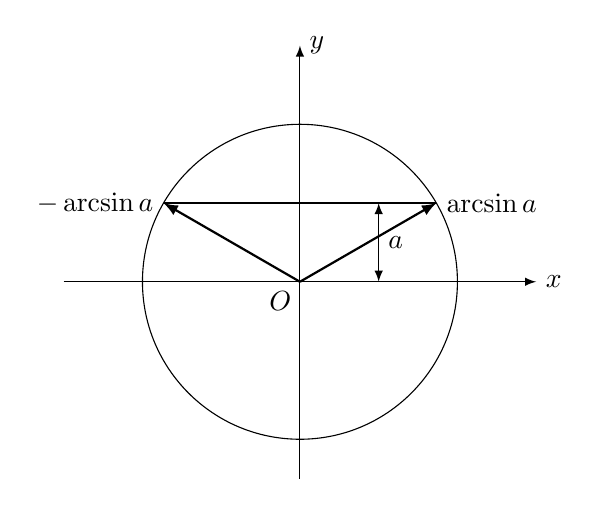
\begin{tikzpicture}[>=latex]
      \draw[->] (-3,0)--(3,0)node[right]{$x$};
      \draw[->] (0,-2.5)--(0,3)node[right]{$y$};
      \node at (-.25,-.25){$O$};
      \draw (0,0) circle(2);
      \draw[thick,->] (0,0)--(30:2)node[right]{$\arcsin a$};
      \draw[thick,->] (0,0)--(150:2)node[left]{$\uppi-\arcsin a$};
      \draw (30:2)--(150:2);
      \draw[<->] (1,0)--node[right]{$a$}(1,1);
    \end{tikzpicture}
    \caption{}\label{fig:unit_circle_solution1}
  \end{figure}

  当 $\arcsin a<x<\uppi-\arcsin a$ 时,$f(x)=\sin x-a>0$ 成立;

  当 $-\dfrac{\uppi}{2}<x<\arcsin a$ 或 $\uppi-\arcsin a<x<\dfrac{3\uppi}{2}$ 时,$f(x)=\sin x-a<0$ 成立,因此,在 $|a|\leqslant 1$ 的场合,$\sin x>a$ 在 $\left[-\dfrac{\uppi}{2}, \dfrac{3\uppi}{2}\right]$ 内的解满足条件:
  \[\arcsin a<x<\uppi-\arcsin a\]
  由于 $f(x)=\sin x-a$ 是周期等于 $2\uppi$ 的函数,因此 $\sin x>a$ 的一切解满足条件:
  \[2k\uppi+\arcsin a<x<(2k+1)\uppi-\arcsin a,\quad k\in\mathbb{Z}\]
  \item 若 $a>1$, 则对于任何 $x\in\mathbb{R}$,有 $f(x)=\sin x-a<0$,因此,不等式 $\sin x>a$ 没有解。
  \item 若 $a<-1$,则对于任何 $x\in\mathbb{R}$,有 $f(x)=\sin x-a>0$,因此,不等式 $\sin x>a$ 的解集是实数集 $\mathbb{R}$。
\end{enumerate}

总之:
\begin{enumerate}
  \item 当 $|a|\leqslant 1$ 时,所求不等式的解集是
  \[\{x|2k\uppi+\arcsin a<x<(2k+1)\uppi-\arcsin a\}\]
  \item 当 $a>1$ 时,所求不等式的解集是空集 $\emptyset$;
  \item 当 $a<-1$ 时,所求不等式的解集是实数集 $\mathbb{R}$。
\end{enumerate}
\end{solution}

\begin{example}
  解不等式 $\cos x<a$
\end{example}

\begin{solution}
移项,化为 $\cos x-a<0$

设 $f(x)=\cos x-a$,$f(x)$ 是周期等于 $2\uppi$ 的函数,先讨论在长度等于一个周期的区间 $[-\uppi,\uppi]$ 内的 $f(x)$ 的符号:
\begin{enumerate}
  \item 若 $|a|\leqslant 1$,$f(x)=\cos x-a$ 在 $[-\uppi,\uppi]$ 内的解是
  \[x_1=\arccos a\quad \text{和}\quad x_2=-\arccos a\]
  把解的终边画在单位圆上,如\cref{fig:unit_circle_solution2} 且由\cref{fig:unit_circle_solution2} 容易
看出:
  \begin{figure}
    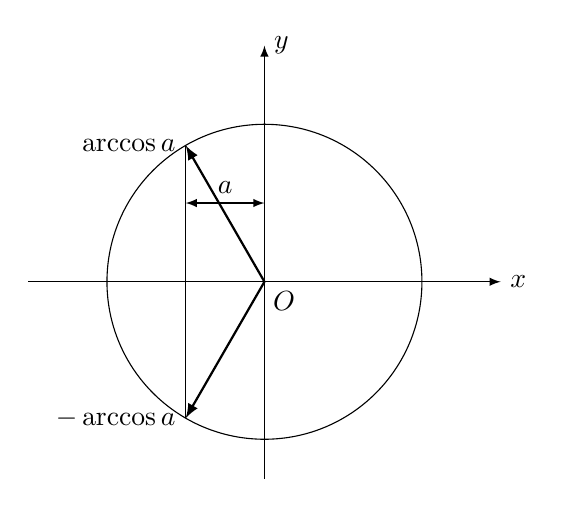
\begin{tikzpicture}[>=latex]
      \draw[->] (-3,0)--(3,0)node[right]{$x$};
      \draw[->] (0,-2.5)--(0,3)node[right]{$y$};
      \node at (.25,-.25){$O$};
      \draw (0,0) circle(2);
      \draw[thick,->] (0,0)--(120:2)node[left]{$\arccos a$};
      \draw[thick,->] (0,0)--(-120:2)node[left]{$-\arccos a$};
      \draw (120:2)--(-120:2);
      \draw[<->] (0,1)--node[above]{$a$}(-1,1);
    \end{tikzpicture}
    \caption{}\label{fig:unit_circle_solution2}
  \end{figure}

当 $\arccos a<x<\uppi$ 或 $-\uppi <x<-\arccos a$ 时,$f(x)=\cos x-a<0$ 成立,而且仅在此时成立,又因为 $f(x)=\cos x-a$的周期是 $2\uppi$,所以,$\cos x<a$ 的一切解,满足
\begin{equation}
  \label{eq:solution_cos_negative}
   2k\uppi +\arccos a<x<(2k+1)\uppi  
\end{equation}
或
\begin{equation}
  \label{eq:solution_cos_positive}
    (2k-1)\uppi <x<2k\uppi -\arccos a
\end{equation}
又\cref{eq:solution_cos_positive} 也可以写成
\begin{equation}
  \label{eq:solution_cos_positive2}
    (2k+1)\uppi <x<(2k+2)\uppi -\arccos a
\end{equation}
再将\cref{eq:solution_cos_negative,eq:solution_cos_positive2} 合并为
\begin{equation}
  \label{eq:solution_cos}
  2k\uppi +\arccos a<x<(2k+2)\uppi -\arccos a
\end{equation} 
因此,在 $|a|\leqslant 1$ 的场合,$\cos x<a$ 的一切解满足 \eqref{eq:solution_cos}。

\item 若 $a>1$,则对于任何 $x\in\mathbb{R}$,有$f(x)=\cos x-a<0$ 成立,因此,不等式 $\cos x<a$ 的解集是实数集 $\mathbb{R}$。
\item 若$a<-1$,则对于任何 $x\in\mathbb{R}$,有 $f(x)=\cos x-a>0$ 成立,因此,不等式 $\cos x<a$ 没有解。
\end{enumerate}

总之,
\begin{enumerate}
  \item 当 $|a|\leqslant 1$ 时,所求不等式的解集是
  \[\{x|2k\uppi  +\arccos a<x<(2k+2)\uppi -\arccos a\}\]
  \item 当 $a>1$ 时,所求不等式的解集是实数集 $\mathbb{R}$。
  \item 当 $a<-1$ 时,所求不等式的解集是空集 $\emptyset$。
\end{enumerate}
\end{solution}


\begin{example}
  解不等式 $2\cos^2 2x<1$
\end{example}

\begin{solution}
移项,化简为 $\cos4x<0$。设 $f(x)=\cos4x$,它是周期等于 $\dfrac{2\uppi}{4}=\dfrac{\uppi}{2}$ 的函数。

$f(x)=\cos4x$ 在 $\left[0,\dfrac{\uppi}{2}\right]$ 内的零点为 $\dfrac{\uppi}{8}$,$\dfrac{3\uppi}{8}$。

显然,当 $0\leqslant x<\dfrac{\uppi}{8}$ 时,$f(x)=\cos4x>0$;当 $\dfrac{\uppi}{8}<x<\dfrac{3\uppi}{8}$ 时,$f(x)=\cos4x<0$;当 $\dfrac{3\uppi}{8}<x\leqslant \dfrac{\uppi}{2}$ 时,$f(x)=\cos4x>0$。

$\therefore\quad \cos4x<0$ 在 $\left[0,\dfrac{\uppi}{2}\right]$ 内的部分解满足条件:$\dfrac{\uppi}{8}<x<\dfrac{3\uppi}{8}$

又 $f(x)$ 的周期是 $\dfrac{\uppi}{2}$。

$\therefore\quad \cos4x<0$ 的一切解满足条件
\[\frac{\uppi}{8}+n\cdot\frac{\uppi}{2}<x<\frac{3\uppi}{8}+n\cdot\frac{\uppi}{2}\qquad (n\in\mathbb{Z})\]
$\therefore\quad 2\cos^2 2x<1$ 的解集是
\[\left\{x\Big| \frac{\uppi}{8}+n\cdot\frac{\uppi}{2}<x<\frac{3\uppi}{8}+n\cdot\frac{\uppi}{2}\right\}\]
\end{solution}


\begin{example}
  解不等式 $\dfrac{\cos2x+\cos x-1}{\cos2x}>2,\quad (0<x<2\uppi)$
\end{example}

\begin{solution}
移项,并将 $\cos2x=2\cos^2x-1$ 代入得
\[\frac{\cos x(1-2\cos x)}{2\cos^2x-1}>0\] 
因为原不等式的解使 $\cos2x\ne 0$(即 $2\cos^2x-1\ne 0$),两边乘以 $(2\cos^2x-1)^2$,得到同解不等式
\[\cos x(1-2\cos x)(2\cos^2x-1)>0\]
即
\[\left(\cos x+\frac{1}{\sqrt{2}}\right)\cos x\left(\cos x-\frac{1}{2}\right)\left(\cos x-\frac{1}{\sqrt{2}}\right)<0\]
上面不等式右端的函数式 $f(x)$ 的零点依大小排列是 $-\dfrac{1}{\sqrt{2}},\; 0,\; \dfrac{1}{2},\; \dfrac{1}{\sqrt{2}}$。由此得知,仅当
\begin{equation}
  \label{eq:solution_quadrant2}
  -\frac{1}{\sqrt{2}}<\cos x<0
\end{equation}
或
\begin{equation}
  \label{eq:solution_quadrant1}
  \frac{1}{2}<\cos x<\frac{1}{\sqrt{2}}
\end{equation}
时,$f(x)=\cos x(1-2\cos x)(2\cos^2x-1)<0$。

由于 $\cos x$ 在区间 $[0,\uppi]$ 内是递减的,在区间 $[\uppi,2\uppi]$ 内
是递增的,所以由不等式 \eqref{eq:solution_quadrant2}, 得(\cref{fig:solution_negative}):
\[\frac{\uppi}{2}<x<\frac{3\uppi}{4},\qquad \frac{5\uppi}{4}<x<\frac{3\uppi}{2}\]
由不等式 \eqref{eq:solution_quadrant1}, 得(\cref{fig:solution_positive}):
\[\frac{\uppi}{4}<x<\frac{\uppi}{3},\qquad \frac{5\uppi}{3}<x<\frac{7\uppi}{4}\]
因此,原不等式在区间 $0<x<2\uppi$ 内的解集是
\[\left\{x\Big|\frac{\uppi}{4}<x<\frac{\uppi}{3} \right\}\bigcup\left\{x\Big|\frac{\uppi}{2}<x<\frac{3\uppi}{4} \right\}\bigcup\left\{x\Big|\frac{5\uppi}{4}<x<\frac{3\uppi}{2} \right\}\bigcup\left\{x\Big|\frac{5\uppi}{3}<x<\frac{7\uppi}{4} \right\}\]
\end{solution}

\begin{figure}
  \begin{minipage}[t]{0.48\textwidth}
    \centering
    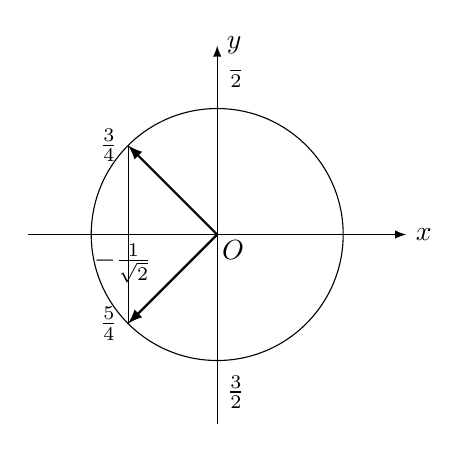
\begin{tikzpicture}[>=latex, scale=.8]
      \draw[->] (-3,0)--(3,0)node[right]{$x$};
      \draw[->] (0,-3)--(0,3)node[right]{$y$};
      \node at (.25,-.25){$O$};
      \draw (0,0) circle(2);
      \draw[thick,->] (0,0)--(135:2)node[left]{$\frac{3\uppi}{4}$};
      \draw[thick,->] (0,0)--(-135:2)node[left]{$\frac{5\uppi}{4}$};
      \draw (135:2)--(-135:2);
      \node at (0,2.5)[right]{$\frac{\uppi}{2}$};
      \node at (0,-2.5)[right]{$\frac{3\uppi}{2}$};
      \node at (-1.5,0)[below]{$-\frac{1}{\sqrt{2}}$};
    \end{tikzpicture}
    \caption{}\label{fig:solution_negative}
  \end{minipage}
  \begin{minipage}[t]{0.48\textwidth}
    \centering
    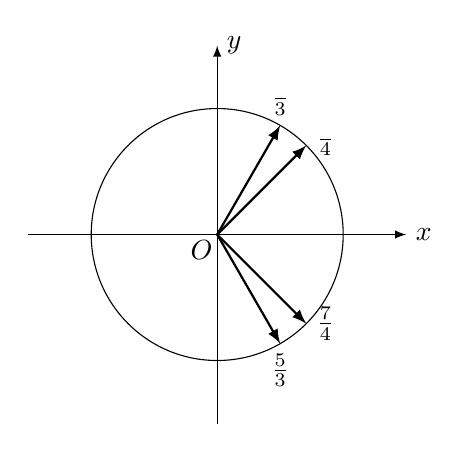
\begin{tikzpicture}[>=latex, scale=.8]
      \draw[->] (-3,0)--(3,0)node[right]{$x$};
      \draw[->] (0,-3)--(0,3)node[right]{$y$};
      \node at (-.25,-.25){$O$};
      \draw (0,0) circle(2);
      \draw[thick,->] (0,0)--(45:2)node[right]{$\frac{\uppi}{4}$};
      \draw[thick,->] (0,0)--(-45:2)node[right]{$\frac{7\uppi}{4}$};
      \draw[thick,->] (0,0)--(60:2)node[above]{$\frac{\uppi}{3}$};
      \draw[thick,->] (0,0)--(-60:2)node[below]{$\frac{5\uppi}{3}$};
    \end{tikzpicture}
    \caption{}\label{fig:solution_positive}
  \end{minipage}
\end{figure}

\begin{Exercise}
\begin{question}
  \item 解下列方程:
  \begin{tasks}(2)
    \task $\sin x=1$
    \task $\sin x=0$
    \task $\cos x=0$
    \task $\cos x=1$
    \task $\cot x=0$
    \task $\sin x=\dfrac{\sqrt{3}}{2}$
    \task $\sin\left(x+\dfrac{\uppi}{6}\right)=-\dfrac{1}{2}$
    \task* $\cos\left(x+\dfrac{\uppi}{6}\right)=\dfrac{1}{2}$
    \task $\tan \left(x-\dfrac{\uppi}{3}\right)=-\sqrt{3}$
    \task $\tan \left(x+\dfrac{\uppi}{4}\right)=-1$
    \task $\cot \dfrac{2x}{3}-1=0$
    \task $\cos\left(x+\dfrac{\uppi}{4}\right)=-\dfrac{\sqrt{3}}{2}$
  \end{tasks}
  \item 解下列各方程(用反三角函数符号表示各方程的解):
  \begin{tasks}(2)
    \task $\sin2x=0.7$
    \task $\tan 3x=3$
    \task $\cot (2x-1)=\sqrt{2}$
    \task $\cos\dfrac{\alpha}{2}=\dfrac{1}{5}$
    \task $\cot \dfrac{x}{4}=\dfrac{1}{4}$
    \task $\sin\left(\alpha+\dfrac{\uppi}{3}\right)=0.1$
    \task $\cos\left(2x-\dfrac{\uppi}{10}\right)=0.85$
    \task $\tan \left(\dfrac{x}{2}+\dfrac{\uppi}{5}\right)=\dfrac{1}{8}$
  \end{tasks}
  \item 解下列各方程:
  \begin{tasks}(2)
    \task $2 \sin \dfrac{x+1}{4}+1=0$
    \task $4 \sin ^{2} 4 x-3=0$
    \task $2 \sin ^{2} x-3 \sin x+1=0$
    \task $\tan ^{2} 3 x=2 \tan  3 x$
    \task! $\cot^{2}\left(\dfrac{x}{2}-\dfrac{\uppi}{8}\right)+3 \cot\left(\dfrac{x}{2}-\dfrac{\uppi}{8}\right)-4=0$
    \task  $4 \cos ^{2} x+\sin x=1$
    \task  $\tan  x+5 \cot x=6$
    \task  $2 \cot 3 x+\tan  3 x+3=0$
  \end{tasks}
  \item $a,b,c$ 满足什么条件,方程 $a\sin^2 x+b\cos^2 x=c$ 有解。
  \item 解下列各方程:
  \begin{tasks}(2)
    \task  $\sin x(1+2 \cos x)=0$
    \task  $\sin 2 x \cos 3 x=0$
    \task  $\cos \left(2 x+\dfrac{\uppi}{3}\right) \sin \left(3 x-\dfrac{\uppi}{3}\right)=0$
    \task  $\cos 5 x(1+\cos 2 x)=0$
    \task! $\cot x-\cos x=1-\sin x$
    \task! $1+\sin x \cos 3 x+\sin x+\cos 3 x=0$
    \task  $\dfrac{\cos x}{1+\sin x}=2-\tan x$
    \task  $\sin 3 x \cdot \cot x=0$
  \end{tasks} 
  \item 解下列各方程:
  \begin{tasks}(2)
    \task   $\sin 3 x=\cos 3 x$
    \task   $\sin ^{2} 3 x=3 \cos ^{2} 3 x$
    \task!  $ 5 \cos x+2 \sin x=5 \cos x \cos 2 x+2 \sin x \cos 2 x$   
    \task!  $\sin x \tan x+\cos x \cdot \cot x=\sin x+\cos x$
    \task!  $\sin ^{2} x+5 \sin x \cos x+4 \cos ^{2} x=0$
    \task! $3 \sin ^{2} x-7 \sin x \cos x+6 \cos ^{2} x=1$
    \task!  $\dfrac{\sin x+2 \cos x}{\sin x-2 \cos x}=3$
    \task!  $\dfrac{2 \sin ^{2} x-4 \cos ^{2} x}{\sin ^{2} x+3 \sin x \cos x+6 \cos ^{2} x}=1$
  \end{tasks}
  \item $a, b$ 满足什么条件, 方程 $\dfrac{a^{2} \sin x^{2}+b \cos x^{2}}{b^{2} \sin ^{2} x+a \cos x}=1$ 有解。
  \item 解下列各方程:
  \begin{tasks}(2)
    \task  $\sin 3 x \cos x=\cos 3 x \sin x$
    \task  $\cos 7 x \cos 3 x=\cos 4 x$
    \task! $\sin \left(\dfrac{\uppi}{2}-x\right) \cos 2 x+\sin (2 x-\uppi) \sin x=0$
    \task! $\sin \dfrac{3 \uppi-x}{2} \cos \left(\dfrac{\uppi}{2}-3 x\right) =\cos (3 x-\uppi) \cos \dfrac{3 \uppi+x}{2}$
    \task  $\tan x\cdot \tan\left(3x-\dfrac{\uppi}{4}\right)=1$
    \task  $\sin x\cos x=\dfrac{1}{4}$
    \task  $\sin(\ang{34}+x)\sin(\ang{56}-x)=\dfrac{\sqrt{2}}{4}$
    \task  $\cos^4x-\sin^4x=1$
    \task! $\cos ^{2}\left(x+\ang{30}\right)-\sin ^{2}\left(x+\ang{30}\right)=\dfrac{1}{2}$
    \task! $\sin \left(x+\dfrac{\uppi}{10}\right) \sin \left(\dfrac{2 \uppi}{5}-x\right)=\dfrac{\sqrt{2}}{4}$
    \task  $\sin \left(x+\dfrac{\uppi}{6}\right)=2 \cos x$
    \task  $1-\tan^{2} x=2 \tan x \tan 2 x$
    \task  $2 \cos 2 x=7 \sin x $
    \task  $\sin 2 x+\sqrt{2} \sin x=0$
    \task  $2 \sin ^{2} x+\sin ^{2} 2 x=2$
    \task  $\dfrac{\cos 2 x}{\cos x-\sin x}=0$
    \task  $\sin 4 x=2 \cos ^{2} x-1 $
    \task  $\sin x \cos x \cos 2 x=\dfrac{1}{8}$
    \task  $\cot x-\tan x=\tan 2 x$
    \task  $2-\sin \dfrac{x}{2}=2 \cos \dfrac{x}{2}$
  \end{tasks}
  \item 解下列各方程:
  \begin{tasks}(2)
    \task  $\sin 2 x=\sin 3 x$
    \task  $\cos \left(2 x+\ang{15}\right)=\cos \left(4 x-\ang{15}\right)$
    \task  $\tan\left(\dfrac{x}{2}+\ang{30}\right)=\tan\left(2 x+\ang{60}\right)$
    \task  $\cos 3 x=\sin \left(x-\dfrac{\uppi}{6}\right)$,
    \task  $\tan\left(\dfrac{\uppi}{8}-x\right)=\cot\left(\dfrac{\uppi}{4}+3 x\right)$
    \task  $\sin 2 x=-\sin \dfrac{x}{2}$
    \task  $\tan 3 x+\cot \dfrac{x}{3}=0$
    \task  $\sin 3 x+\dfrac{\sqrt{3}}{2} \sin 2 x=\dfrac{1}{2} \cos 2 x$
    \task  $\cos x-\sin x=1$
    \task  $2 \cos \left(x+\ang{20}\right) \cos x=\cos \ang{40} $
    \task  $\sin x+\cos x=2 \sqrt{2} \sin x \cos x$
    \task  $\sin 3 x \cos x=\sin 7 x \cos 5 x$
    \task! $\cos \left(2 x+\ang{15}\right)+\cos \left(2 x-\ang{15}\right)=\dfrac{1}{2}$
    \task!  $\sin \left(2 x+\dfrac{\uppi}{18}\right) \cos \left(2 x-\dfrac{\uppi}{9}\right)=-\dfrac{1}{4}$
    \task! $\sin \left(x+\ang{15}\right) \sin \left(x-\ang{30}\right)=$ $\sin \left(\ang{50}+x\right) \cos \left(\ang{85}-x\right)$
  \end{tasks}
  \item 解下列各方程:
  \begin{tasks}(2)
    \task $\cos 7 x+\cos x=\cos 4 x$
    \task $\tan x+\tan 2 x=\sin 3 x \cos x$
    \task $\cos 8 x+\cos 6 x=\sqrt{3} \cos x$
    \task $1-\cos 2 x=4 \sin x$
    \task $\sin x+\sin 2x+ \sin 3x= 0$
    \task $\cos x+\cos2x-\cos3x=1$
    \task $\sin2 x+2\sin x=\sin\dfrac{x}{2}$
    \task $1+\cos2x+\sin x=2\cos^2\dfrac{x}{2}$
    \task $\tan x+\tan 2x=\tan 3x$
  \end{tasks}
  \item 解下列各方程:
  \begin{tasks}(2)
    \task $\sin ^{2}\left(x+10^{\circ}\right)-\sin ^{2} x=\dfrac{1}{2} \sin 20^{\circ}$
    \task $\sin ^{2} x+\sin ^{2} 2 x+\sin ^{2} 3 x=\dfrac{3}{2}$
    \task $\cos ^{2} x+\cos ^{2} 2 x+\cos ^{2} 3 x=1$
    \task $\sin ^{2} 2 x+\sin ^{2} 4 x=\dfrac{3}{2}$
    \task $\sqrt{3} \cos x+\sin x=\sqrt{3} $
    \task $4 \sin x+3 \cos x=2 $
    \task $\sin 3 x+2 \cos 2 x=1 $
    \task! $5 \cos \left(2 x+18^{\circ}\right)-12 \sin \left(2 x+18^{\circ}\right)=13$
    \task! $(4 \sin x-5 \cos x)^{2}-13(4 \sin x-5 \cos x)+42=0$
  \end{tasks}
  \item 解下列方程:
  \begin{tasks}(2)
    \task $\dfrac{1+\tan x}{1-\tan x}=1+\sin 2 x$
    \task $\dfrac{\sin x}{1+\cos x}=2-\cot x$
    \task $\sin 2 x=\cos 2 x-\sin ^{2} x+1$
    \task! $(\cos 5 x+\cos 7 x)^{2}=(\sin 5 x+\sin 7 x)^{2}$
  \end{tasks}
  \item 设关于 $x$ 的方程 $\sin x+\sqrt{3}\cos x+a=0$ 在区间内有相异二解 $\alpha,\beta$。 试求常数 $a$ 的取值范围和 $\tan(\alpha+\beta)$ 的值。
  \item 解下列各方程组:
  \begin{tasks}(2)
    \task $\begin{cases}
        \sin x\sin y=\dfrac{1}{4\sqrt{2}}\\
        \tan x\cdot \tan y=\dfrac{1}{3}
    \end{cases}$
    \task $\begin{cases}
        x+y=\dfrac{\uppi}{4}\\
        \tan x+\tan y=1
    \end{cases}$
    \task $\begin{cases}
        \sin(2x+\sin^2y)=0\\
        x-3\sin^2y=-2
    \end{cases}$
  \end{tasks}
  \item 解下列的不等式:
  \begin{tasks}(2)
    \task $\sin (2 \uppi \cos x)>0$
    \task $\lg \sin x \leqslant 0$
    \task $\cos ^{2} x+7 \sin ^{2} x<8 \sin x \cos x$
    \task $\sin x+\sqrt{3} \cos x>1$
    \task! $2 \cos ^{2}\left(x+30^{\circ}\right)-3 \sin \left(60^{\circ}-x\right)+1>0$
  \end{tasks}
  \item 求下列各函数的定义域:
  \begin{tasks}(2)
    \task $y=\arccos \dfrac{3}{x}$
    \task $y=\arcsin \dfrac{2 x}{1+x^{2}}$
    \task $y=\sqrt{\sin x}$
    \task $y=\sqrt{4 \cos ^{2} 2 x-3}$
  \end{tasks} 
\end{question}
\end{Exercise}
\chapter{指数函数与对数函数}
\section{有理指数函数}
在本教材第三册中,已经把指数幂的定义范围从正整指数逐步推广到“负整数”,“正、负分数”,在逐步推广过程中,我们始终遵守的指导原则是保有指数法则:
\[a^m\cdot a^n=a^{m+n},\qquad  (a^m)^n=a^{m\cdot n}\]
指数在有理数系 $\mathbb{Q}$ 内,我们有下面的指数幂的定义:
\[\begin{split}
  a^n=\underbrace{a\cdot a\cdot a\cdots a}_{\text{$n$个$a$}},&\qquad (n\in\mathbb{N})\\  
a^0=1,&\qquad (a\ne 0)\\  
a^{-n}=\frac{1}{a^n},&\qquad (a\ne 0)\\ 
a^{\tfrac{m}{n}}=\sqrt[n]{a^m}=\left(\sqrt[n]{a}\right)^m,&\qquad (a\geqslant 0,\; m,n\in\mathbb{N})\\ 
a^{-\tfrac{m}{n}}=\frac{1}{a^{\tfrac{m}{n}}},&\qquad (a> 0)\\ 
\end{split}\]
采用上面定义后,我们在第三册中也证明了正实数 $a$ 和 $b$ 的有理指数幂依然满足指数运算法则:
\[a^{\alpha}\cdot a^{\beta}=a^{\alpha+\beta},\qquad (a^{\alpha})^{\beta}=a^{\alpha\beta},\qquad (a\cdot b)^{\alpha}=a^{\alpha}\cdot b^{\alpha}\]
这里 $\alpha,\beta \in \mathbb{Q}$。

这样一来,函数 $a^x\; (a>0)$ 对于任意有理数 $x$ 都有定义了。我们称它为有理指数函数,这个函数具有上面所说的三个性质。下面将进一步研讨这个函数的其它重要性质:

\begin{Theorem}{性质 1}
\begin{enumerate}
  \item 若 $a>1$,当有理数 $x>0$ 时,则 $a^x>1$,当有理数 $x<0$ 时,则 $a^x<1$。
  \item 若 $0<a<1$,当有理数 $x>0$ 时,则 $a^x<1$,当有理数 $x<0$ 时,则 $a^x>1$。
\end{enumerate}
\end{Theorem}

\begin{proof}
\begin{enumerate}
\item 若 $a>1$,
\begin{enumerate}
  \item 设 $x=\frac{m}{n}>0,\; (m,n\in\mathbb{N})$,则 $a^x=a^{\tfrac{m}{n}}=\sqrt[n]{a^m}$,因为 $a>1$,所以 $a^m>1$ (幂函数 $f(x)=x^m$ 在
$[0,+\infty)$ 上是严格递增的),又 $\sqrt[n]{a^m}>1$(幂函数 $f(x)=x^{\tfrac{1}{n}}$ 在 $[0,+\infty)$ 上是严格递增的),即 $a^x>1$。
\item 设 $x<0$,$x=-x_1,\; (x_1>0)$,则 $0<a^x=a^{-x_1}=\dfrac{1}{a^{x_1}}<1$,($\because\; a^{x_1}>1$)。
\end{enumerate}
 
\item 若 $0<a<1$,
\begin{enumerate}
  \item 设 $a=\dfrac{1}{a_1},\; a_1>1$,则当 $x>0$,$a^x=\left(\dfrac{1}{a_1}\right)^x=\dfrac{1}{a^x_1}<1$,($\because\; a_1^{x}>1$)。
  \item 设 $x<0$,$x=-x_1,\; (x_1>0)$ 则
$a^x=a^{-x_1}=\dfrac{1}{a^{x_1}}>1$,($\because\; a^{x_1}<1$)。
\end{enumerate}
\end{enumerate}
\end{proof}

\medskip
性质 1 的几何意义表明:当 $a>1$ 时,有理指数函数 $y=a^x$ 的图象上的点在有单斜线的区域 I 和 II 的部分;当 $0<a<1$ 时,$y=a^x$ 的图象上的点在有双斜线的区域 III 和 IV 的部分(\cref{fig:lg_region})。

\begin{figure}[htp]
  \centering
\begin{tikzpicture}[>=latex, scale=.85]
\draw[->] (-3,0)--(4,0)node[right]{$x$};
\draw[->] (0,-1)--(0,5)node[right]{$y$};
\node at (-.25,-.25){$O$};
\draw[very thick](-3,1)--(3.5,1)node[right]{$y=1$};
\fill[pattern = north east lines] (-3,1)  rectangle (0,0);
\fill[pattern = north east lines] (3,4.5)  rectangle (0,0);
\fill[pattern = crosshatch] (-3,4.5)  rectangle (0,1);
\fill[pattern = crosshatch] (3,1)  rectangle (0,0);
\node[rectangle,fill=white] at (1.5,3){I};
\node[rectangle,fill=white] at (-1.5,0.5){II};
\node[rectangle,fill=white] at (-1.5,3){III};
\node[rectangle,fill=white] at (1.5,0.5){IV};
\end{tikzpicture}
  \caption{}\label{fig:lg_region}
\end{figure}

\begin{Theorem}{性质 2}
\begin{enumerate}
  \item 若 $a>1$,$x_1<x_2$,则 $a^{x_1}<a^{x_2}$,即底数大于 1 的有理指数函数 $a^x$ 是递增的;
  \item 若 $0<a<1$,$x_1<x_2$,则 $a^{x_1}>a^{x_2}$,即底数小于 1 的正数的有理指数函数 $a^x$ 是递减的。
\end{enumerate}
\end{Theorem}

\begin{proof}
  若 $a>1$ 和 $x_1<x_2$,那么
\[a^{x_2}-a^{x_1}=a^{x_1}\left(\frac{a^{x_2}}{a^{x_1}}-1\right)=a^{x_1}\left(a^{x_2-x_1}-1\right)\]
  
因为 $x_2-x_1>0$,$a>1$,所以 $a^{x_2-x_1}>1$,又 $a^{x_1}>0$。因此,$a^{x_2-x_1}>0$,即 $f(x)=a^x,\; (a>1)$ 是递增的。

若 $0<a<1$ 和 $x_1<x_2$,那么
\[a^{x_2}-a^{x_1}=a^{x_1}\left(a^{x_2-x_1}-1\right)\]
因为 $x_2-x_1>0$,$0<a<1$,所以 $a^{x_2-x_1}<1$,又 $a^{x_1}>0$,因此 $a^{x_2-x_1}<0$,即 $f(x)=a^x,\; (0<a<1)$ 是递减的。
\end{proof}

我们现在的任务是要把有理指数函数开拓为一个定义在实数集上的连续函数。能否做到这一点的关键是如何对全体无理点补充定义,使得指数函数在整个实数轴 $\mathbb{R}$ 上处处连续。为此,我们先说明有理指数函数的一个极限性质。


\begin{Theorem}{性质 3}
  设 $a>0$,则当 $n\to +\infty$ 时,数列 $\left\{a^{\tfrac{1}{n}}\right\}$ 的极限是 1,即
  \[\lim_{n\to\infty}a^{\tfrac{1}{n}}=1\]
\end{Theorem}

\begin{proof}
\begin{enumerate}
  \item 当 $a=1$ 时,结论自然成立。
  \item 当 $a>1$ 时,因为 $\dfrac{1}{n}>0$,所以 $a^{\tfrac{1}{n}}>1$(性质 1),设 $a^{\tfrac{1}{n}}=1+h$,其中 $h>0$,两边 $n$ 次方,得到
  \[ a=(1+h)^n\]
 
  由贝努利不等式得
  \[ a=(1+h)^n>1+nh\]
  所以,$0<h<\dfrac{a-1}{n},\qquad 1<1+h<1+\dfrac{a-1}{n}$, 即:
  \[1<a^{\tfrac{1}{n}}<1+\dfrac{a-1}{n}\]  
  再令 $n\to +\infty$,由上式就得到
  \[1\leqslant \lim_{n\to\infty}a^{\tfrac{1}{n}}\leqslant 1 \]
  因此
  \[\lim_{n\to\infty}a^{\tfrac{1}{n}}=1\]
  \item 当 $0<a<1$ 时,令 $a=\dfrac{1}{b}$,则 $b>1$,由上面的证明得到
  \[\lim_{n\to\infty}b^{\tfrac{1}{n}}=1\]
  于是
  \[\begin{split}
    \lim_{n\to\infty}a^{\tfrac{1}{n}}&=\lim_{n\to\infty}\left(\frac{1}{b}\right)^{\tfrac{1}{n}}=\lim_{n\to\infty}\frac{1}{b^{\tfrac{1}{n}}}\\
    &=\frac{1}{\displaystyle\lim_{n\to\infty}b^{\tfrac{1}{n}}}=\frac{1}{1}=1
  \end{split}\]
\end{enumerate} 
\end{proof}

性质 3 可以进一步推广到下面的推论:

\begin{Deduction}{推论}
若 $a>0$ 且 $a\ne 1$,有理数数列 $\{h_i\},\; i=1,2,3,\ldots$,以 0 为极限,即 $\lim\limits_{i\to\infty}h_i=0$,那么
\[\lim_{i\to\infty}a^{h_i}=1\]
\end{Deduction}

\begin{proof}
先设 $a>1$,因为 $\lim\limits_{i\to\infty}h_i=0$,必定存在这样的自然数 $N$,使得当 $i\geqslant N$ 时,$|h_i|<1$,从而 $\dfrac{1}{|h_i|}>1$。用 $m_i$ 表示 $\left[\dfrac{1}{|h_i|}\right]$,即不大于 $\dfrac{1}{|h_i|}$ 的最大整数,于是
\begin{equation}
  m_i=\left[\frac{1}{|h_i|}\right]\leqslant\frac{1}{|h_i|}<m_i+1
\end{equation}
所以,当 $i\geqslant N$ 时,有
\[\frac{1}{m_i+1}<|h_i|\le\frac{1}{m_i}\]
由 $h\to 0$ 知,$\dfrac{1}{|h_i|}\to \infty$。 从而由 $m_i+1>\dfrac{1}{|h_i|}$ 知,$m_i\to\infty$。根据有理指数幂的单调性,得
\[1<a^{|h_i|}<a^{\tfrac{1}{m_i}},\qquad (a>1)\]

仿照性质 3 的证明,令 $b_i=a^{\tfrac{1}{m_i}}-1>0$,于是,
\[\begin{split}
  a^{\tfrac{1}{m_i}}&=(1+b_i)\\
  a&=(1+b_i)^{m_i}>1+m_ib_i\\
  & 0<b_i<\frac{a-1}{m_i}
\end{split}\]
当 $i\to 0$ 时,$m_i\to \infty$,

$\therefore\quad b_i\to 0$,即$a^{h_i}\to 1$, 从而当$i\to \infty$时,$|h_i|\to 0$,$a^{|h_i|}\to 1$,即$a^{h_i}\to 1$。

若 $0<a<1$,令 $b=\dfrac{1}{a}>1$,于是
\[\lim_{i\to \infty} a^{h_i}=\lim_{i\to \infty} \left(\frac{1}{b}\right)^{h_i}=\frac{1}{\lim\limits_{i\to \infty} b^{h_i}}=\frac{1}{1}=1\]
\end{proof}

应用这个推论,我们可以说明当有理数 $x$ 的变化够小时,有理指数函数 $f(x)=a^x$ 的变化可以任意小。

\begin{Theorem}{性质 4}
当指数 $x$ 的变化够小时,有理指数函数 $f(x)=a^x$ 的变化可以任意小。
\end{Theorem}

\begin{proof}
设指数 $x$ 从有理数 $x_1$ 变化到有理数 $x_2=x_1+h_i$,($h_i$ 是有理数),且当 $(x_2-x_1)\to 0$ 时,数列 $\{h_i\}$ 以 0 为极限,于是
\[\begin{split}
  \lim_{x_2\to x_1}\left(a^{x_2}-a^{x_1}\right)&=\lim_{i\to \infty}\left(a^{x_1+h_i}-a^{x_1}\right)\\
  &=a^{x_1}\cdot \lim_{i\to \infty}\left(a^{x_i}-1\right)=0
\end{split}\]
这就是说,只要 $|h_i|$ 够小,那么 $|a^{x_2}-a^{x_1}|$ 就小于任意给定的正数 $\varepsilon$。
\end{proof}


综合有理指数函数的性质,我们可以想象出 $y=a^x\; (a>1)$ 的图象如\cref{fig:4-10-2} 所示,但是我们不能用一条连续不断的曲线把它画出来,因为指数 $x$ 取无理数时,$a^x$ 还没有意义,因而在有理指数函数的图象上,处处有空隙。下一节将由有理指数函数的单调性和性质 4, 适当给无理指数幂补充定义使得指数函数在 $\mathbb{R}$ 上处处连续。

\begin{figure}[htp]
  \centering
\begin{tikzpicture}[>=latex, scale=.7]
\draw[->] (-2,0)--(5,0)node[right]{$x$};
\draw[->] (0,-1)--(0,5)node[right]{$y$};
\node at (-.35,-.35){$O$};
\draw[dashed] (-2,1)--(4.5,1)node[right]{$y=1$};
\draw[domain=-2:3.5, samples=30, very thick, dashed]plot(\x, {1.6^(\x)});
\node at (0,1.3)[left]{$(0,1)$};
\node at (3,1.6^3)[right]{$y=a^x,\quad (a>1)$};
\end{tikzpicture}
  \caption{}\label{fig:4-10-2}
\end{figure}

\begin{Exercise}
\begin{question}
  \item 计算下列各式的值:
  \begin{tasks}(2)
    \task  $25^{3 / 2} \cdot 8^{4 / 3}$ 
    \task  $(0.09)^{1 / 2}+64^{2 / 3}+0.125^{2 / 3}-\dfrac{1}{16^{-3/2}}$
    \task  $64^{1.5} \cdot(32)^{0.4} \div\left(\dfrac{9}{25}\right)^{-3/2}$
    \task  $\left(\dfrac{81}{16}\right)^{-0.25}\left(5^{2}-0.1^{2} \cdot\left(\dfrac{1}{4}\right)^{-3}\right)^{2}$
    \task  $\left[\dfrac{3}{9}-\left(\frac{2}{3}\right)^{-1}\right]^{-1}$
    \task  $(\sqrt{2})^{1.5}+\left(11+\frac{\sqrt[5]{5}}{5^{-0.8}}\right)^{-1 / 4}$
    \task!  $\left[\left(\frac{3}{4}\right)^{0}\right]^{-0.5}-7.5(\sqrt{4})^{2}-(-2)^{-4}+81^{0.25}$
    \task!  $\left[\dfrac{1}{4}\left(0.027^{2 / 3}+15 \times 0.0016^{3 / 4}+1\right)\right]^{-1 / 2}$
    \task!  $6\left[\sqrt{3}\left(\sqrt{3}+2 \sqrt{2}+\frac{2}{3^{1 / 2}}\right)\right] \times\left(3^{1 / 2}+2^{1 / 2}\right)^{-2} \times\left(3^{-1}+2^{-1}\right)$
    \task!  若 $a=(2+\sqrt{3})^{-1},\quad  b=(2-\sqrt{3})^{-1}$,计算 $(a+1)^{-1}+(b+1)^{-1}$
  \end{tasks}
  \item  化简下列各式:
  \begin{tasks}(2)
    \task   $b^{1 / 2} b^{1 / 3}$
    \task   $b^{1 / 2} b^{-1 / 3}$
    \task   $b^{-2 / 3} b^{3 / 5} ;$
    \task   $b^{-2 / 3} b^{3 / 5} ;$
    \task   $\sqrt{a} \cdot \sqrt[3]{a} \cdot \sqrt[5]{a}$
    \task   $\left[1-\left(a^{-1} b^{-1}\right)^{-1}\right]^{-2}$
    \task!  $\left[a^{-1 / 2} b^{-1 / 2}+a^{-1 / 6}\left(b^{-5 / 6}-a^{-1 / 3} b^{-1 / 2}\right)\right]^{-3 / 2}$
    \task!  $\frac{\left(a^{-1}+b^{-1}\right)(a+b)^{-1}}{\sqrt[6]{a^{4} \sqrt[5]{a^{-2}}}}$
    \task!  $\frac{a^{2}+a^{-2}-2}{a^{2}-a^{-2}}$
    \task!  $\left(a^{3 / 4}+b^{3 / 4}\right)\left(a^{3 / 4}-b^{3 / 4}\right) /\left(a^{1 / 2}-b^{1 / 2}\right)$
    \task!  $\left(e^{3 / 2}+2+e^{-3 / 2}\right)\left(e^{3 / 2}-2+e^{-3 / 2}\right)$
    \task!  $\left(a^{1 / 3}+a^{-1 / 3}\right)\left(a^{2 / 3}-1+a^{2 / 3}\right)$
    \task!  $\frac{m-n}{m^{1 / 2}-n^{1 / 2}}+\frac{m^{3 / 2}+n^{3/2}}{m^{1 / 2}+n^{1 / 2}}$
    \task!  $\frac{x^{2 p(q+1)}-y^{2 q(p-1)}}{x^{p(q+1)}-y^{q(p-1)}}$
    \task!  $\left(a^{4 / 3}-2+a^{-4 / 3}\right)\left(a^{2 / 3}-a^{-2 / 3}\right)$
    \task!  $\frac{m-n}{m^{1 / 2}-n^{1 / 2}}+\frac{m^{3 / 2}+n^{3/2}}{m^{1 / 2}+n^{1 / 2}}$
    \task!  $\left[\frac{4 a-9 a^{-1}}{2 a^{1 / 2}-3 a^{-1 / 2}}+\frac{a-4+3 a^{-1}}{a^{1 / 2}-a^{-1 / 2}}\right]^{2}$
  \end{tasks}
  \item  解下列各方程:
  \begin{tasks}(2)
    \task  $\sqrt{2 x-3}=4-x$
    \task  $\sqrt{2 x+8}+\sqrt{x+5}=7$
    \task  $x^{-1 / 4}+x^{-1 / 2}-6=0$
    \task  $x^{1 / 2}+x^{-1 / 2}-\frac{10}{3}=0$
    \task!  $\sqrt[n]{(x+1)^{2}}+\sqrt[n]{(x-1)^{2}}=4 \sqrt[n]{x^{2}-1}$
  \end{tasks}
  \item  设 $h_{i}=\dfrac{100}{2i+1},\quad  m_{i}=\left[\dfrac{1}{h_{i}}\right]=\left[\dfrac{2 i+1}{100}\right]$
  \begin{tasks}
    \task 求证数列 $\{h_i\}=\left\{\dfrac{100}{2i+1}\right\}$ 递减,并求使 $h_i=\dfrac{100}{2i+1}<1$ 的 $i$ 的范围;
    \task 当 $i=10,49,50,100,1000$ 时,求 $m_i$ 的值;
    \task 求证当 $i\geqslant 50$ 时,不等式 $1<100^{\tfrac{100}{2i+1}}<100^{\tfrac{1}{m_i}}$ 成立;
    \task 求证:$\lim\limits_{i\to\infty}\left(100^{\tfrac{1}{m_i}}-1\right)=0,\quad \lim\limits_{i\to\infty}100^{h_i}=1$。
  \end{tasks}
\end{question}
\end{Exercise}

\section{无理指数幂的定义}
要把指数幂的定义由有理数推广到实数,自然又得用逼近法。

设 $\beta$ 是一个无理数,我们可以用两个有理数列 $\{r_n\}$,$\{s_n\}$ 去左、右夹逼,即 $r_n\to \beta\leftarrow s_n$,从而 $\lim\limits_{n\to\infty}r_n=\lim\limits_{n\to\infty}s_n=\beta$。 现在的问题是数列 $\{a^{r_n}\},\{a^{s_n}\}$,(这里 $a>0$)的极限是否存在?如果存在的话,我们就可以定义
\[a^{\beta}=\lim_{n\to\infty}a^{r_n}=\lim_{n\to\infty}a^{s_n}\]

从而就可以把有理指数函数 $a^x$ 开拓为在 $\beta$ 点连续的函数:
\[a^x\; (a>0,\; x\in \mathbb{Q}\cup\{\beta\})=\begin{cases}
  a^x\;  (x\in\mathbb{Q})\\
  a^{\beta}=\lim\limits_{n\to\infty}a^{r_n}=\lim\limits_{n\to\infty}a^{s_n}
\end{cases}\]

\begin{Theorem}{引理}
设 $r_{n} \rightarrow \beta \leftarrow s_{n}$,则
\begin{enumerate}
  \item 当 $a>1$ 时,$a^{r_1}\leqslant a^{r_2}\leqslant\cdots\leqslant a^{r_n}\leqslant\cdots \leqslant a^{s_n}\leqslant\cdots\leqslant a^{s_2}\leqslant a^{s_1}$,且$\left(a^{r_n}-a^{s_n}\right)\to 0$
 
  当 $0<a<1$ 时,$a^{r_1}\geqslant a^{r_2}\geqslant \cdots\geqslant a^{r_n}\geqslant \cdots \geqslant a^{s_n}\geqslant \cdots\geqslant a^{s_2}\geqslant a^{s_1}$,且$\left(a^{r_n}-a^{s_n}\right)\to 0$

  \item $\lim a^{r_n}=\lim a^{s_{n}}=A$ (即极限存在) 
\end{enumerate}
\end{Theorem}

\begin{proof}
$a>1$ 和 $0<a<1$ 这两种情形是完全相似的,只是不等式方向反过来罢了,所以下面只讨论 $a>1$ 的情形,($a=1$ 时它的任何方幂都是 1, 所以 $1^{\beta}=1$)。我们只需证明下述两点:
\begin{enumerate}
  \item $a>1$,$s>r$时,则$a^s>a^r$,(性质 2)。
  \item $\because\quad $当$n\to\infty$时,$s_n-r_n=h_n\to 0$,
  
  $\therefore\quad $由性质 4 得
  \[a^{s_n}-a^{r_n}\to 0\]
  由实数完备性,存在一个唯一实数
  \[ A=\lim a^{s_n}=\lim a^{r_n}\]
\end{enumerate}
\end{proof}

\begin{Definition}
设 $\beta$ 是一任意无理数,$r_n\to\beta\leftarrow s_n$ 是 $\beta$ 的左、右夹逼数列,并且 $u>0$,则定义
\[a^{\beta}=\lim a^{r_n}=\lim a^{s_n}\]
\end{Definition}


我们要说明这个定义的合理性,即上述定义和 $\beta$ 的夹逼有理数列的选取无关。

设 $r'_n\to\beta\leftarrow s'_n$ 是另外一对夹逼数列,则
\[r'_n\to\beta \leftarrow s_n,\qquad r_n\to\beta\leftarrow s'_n\]

由上述引理就有
\[\lim a^{r'_n}=\lim a^{s_n}=\lim a^{r_n}=\lim a^{s'_n}\]

在实数轴 $\mathbb{R}$ 上,对每一个无理点,都补充这样的定义,于是我们就把有理指数函数开拓为一个在实数轴上处处有定义的指数函数 $a^x,\; (a>0,\; x\in\mathbb{R})$。

下面我们将证明这样定义的无理指数幂仍满足指数法则。

\begin{Theorem}{定理}
指数法则 $a^{\beta}\cdot a^{\gamma}=a^{\beta+\gamma}$,$\left(a^{\beta}\right)^{\gamma}=a^{\beta\cdot \gamma}$,$(ab)^{\beta}=a^{\beta}\cdot b^{\beta}$ 对于任何实数 $\beta$,$\gamma$ 都成立。
\end{Theorem}
 
\begin{proof}
当 $\beta$,$\gamma$ 是有理数时,上述等式已在本教材第三册第一章给出证明,所以我们只要说明 $\beta$,$\gamma$ 是无理数的情形。

设 $r_n\to\beta\leftarrow s_n$,$c_n\to\gamma\leftarrow d_n$ 分别是 $\beta$,$\gamma$ 的左、右夹逼数列,于是
\[(r_n+c_n)\to \beta+\gamma \leftarrow (s_n+d_n)\]
\[\begin{split}
  a^{\beta+\gamma}&=\lim a^{r_n+c_n}=\lim a^{r_n}\cdot a^{c_n}\\
  &=\lim a^{r_n}\cdot \lim a^{c_n}=a^{\beta}a^{\gamma}
\end{split}\]

现在让我们来证明 $(a^{\beta})^{\gamma}=a^{\beta\cdot \gamma}$(为了讨论的方便,我们只讨论 $a>1,\; \beta ,\gamma>0$ 的情形),

设 $r_n\to \beta \leftarrow s_n,\quad c_n\to \gamma\leftarrow d_n$,$r_n, s_n,c_n,d_n>0$,则有
\[r_n\cdot c_n\to \beta_{\gamma}\leftarrow s_n\cdot d_n\]
根据正分指数的幂函数与有理指数函数的单调性有
\[(a^{r_n})^{c_n}<(a^{\beta})^{c_n}<(a^{\beta})^{\gamma}<(a^{\beta})^{d_n}<(a^{s_n})^{d_n}\]
所以由有理指数法则,得到
\[a^{r_n\cdot c_n}=(a^{\beta})^{c_n}<(a^{\beta})^{\gamma}<(a^{s_n})^{d_n}=a^{s_n\cdot d_n}\]
\[60+(u,.u,p-pus)\]
$\therefore\quad $ 由引理知,存在唯一的极限
\[(a^{\beta})^{\gamma}=\lim a^{r_n\cdot c_n} =\lim a^{s_n\cdot d_n} =a^{\beta\cdot \gamma}\]

最后证明:$(ab)^{\beta}=a^{\beta}\cdot b^{\beta}$,只讨论 $a>1$,$b>1$ 的情形。

$\because\quad a>1,b>1$

$\therefore\quad ab>1$,于是
\[a^{r_n}b^{r_n}=(ab)^{r_n}<(ab)^{\beta}<(ab)^{s_n}=a^{s_n}b^{s_n}\]
\[(ab)^{s_n}-(ab)^{r_n}\to 0\]
因此,$(ab)^{\beta}=\lim a^{r_n}b^{r_n} = \lim a^{r_n}\cdot \lim b^{r_n}=a^{\beta}\cdot b^{\beta}$
\end{proof}

\begin{example}
  \begin{enumerate}
    \item $10^{\sqrt{2}}\cdot 10^{\sqrt{3}}=10^{\sqrt{2}+\sqrt{3}}$
    \item  $\left[\left(\sqrt[3]{2}\right)^{\sqrt{8}}\right]^{\tfrac{\sqrt{2}}{2}}=2^{\tfrac{1}{3}\times 2\sqrt{2}\times\tfrac{\sqrt{2}}{2}}=2^{\tfrac{2}{3}}=\sqrt[3]{4}$
    \item $\left(5^{-\sqrt{2}}a^{\sqrt{8}}b^{\tfrac{\sqrt{2}}{2}}\right)^{\tfrac{\sqrt{2}}{2}}=5^{-1}a^{2}b^{\tfrac{1}{2}} =\dfrac{a^2\sqrt{b}}{5} $
  \end{enumerate}
\end{example}

\section{实指数函数}
总结上节推广的结果,就得到一个对任意实数 $x$ 都有定义的\emph{实指数函数}:
\[f:\mathbb{R}\mapsto \mathbb{R}^+,\qquad \text{这里}\,\, f(x)=a^x,\; (a>0, \; \text{且}a\ne 1)\]

这个函数就叫做\emph{以 $a$ 为底的指数函数}。上节还说明了指数函数是一个满足下面两个性质的连续函数:
\begin{enumerate}
  \item $f(x_1+x_2)=a^{x_1+x_2}=a^{x_1}\cdot a^{x_2}=f(x_1)\cdot f(x_2)$
  \item $f(kx)=a^{kx}=(a^x)^k=[f(x)]^k$
\end{enumerate}

现在,我们还须验证实指数幂保有有理指数幂的一切性质,并且实指数函数是连续的。

\begin{Theorem}{性质 1}
\begin{enumerate}
  \item 若 $a>1$,当 $x>0$ 时,则 $a^x>1$;当 $x<0$ 时,则 $a^x<1$。
  \item 若 $0<a<1$,当 $x>0$ 时,则 $a^x<1$;当 $x<0$ 时,则 $a^x>1$。
\end{enumerate}
\end{Theorem}

\begin{proof}
如果 $x$ 是有理数,我们在第一节中给过证明,这里不再重述,所以我们只要证明 $x$ 是无理数的情形,设 $x>0$,且 $c_n\to x\leftarrow d_n$ 是 $x$ 的有理数夹逼数列。在数列 $\{c_n\}$ 中一定存在某一项 $c_N$ 和它后面的一切项都是正数,不然的话,如果对于所有的 $n$,有 $c_n\leqslant0$,于是 $\lim c_n\leqslant0$ 即 $x\leqslant0$,这和已知的 $x>0$ 矛盾。

令 $c_N>0$,则 $a^{C_N}>a^0=1$,而 $a^x>a^{c_N}>1$,这就证明了 $a^x>1$。

设 $x<0$,$x=-y$,则 $y>0$,$a^x=a^{-y}=\dfrac{1}{a^y}$

$\because\quad a^y>1,\qquad \therefore\quad a^x=\dfrac{1}{a^y}<1$

\bigskip
$0<a<1$ 的情形,留给同学证明。
\end{proof}

\begin{Theorem}{性质 2}
\begin{enumerate}
  \item 若$a>1$且$x_2>x_1$,则$a^{x_2}>a^{x_1}$
  \item 若$0<a<1$且$x_2>x_1$,则$a^{x_2}<a^{x_1}$
\end{enumerate}
\end{Theorem}

\begin{proof}
设$a>1$且$x_2>x_1$,
\[a^{x_2}-a^{x_1}=a^{x_1}\left(a^{x_2-x_1}-1\right)\]
因为$x_2-x_1>0$,于是$a^{x_2-x_1}>1$,因此$a^{x_2}-a^{x_1}>0$。

设$0<a<1$ 且$x_2>x_1$,
\[a^{x_2}-a^{x_1}=a^{x_1}\left(a^{x_2-x_1}-1\right)\]
因为$x_2-x_1>0$,则$a^{x_2-x_1}<1$,因此$a^{x_2}-a^{x_1}<0$。  
\end{proof}

\begin{Theorem}{性质 3}
\[\lim_{x\to 0} a^x=1\]
\end{Theorem}


对这个极限的证明可以仿照第一节中性质 3 的推论的证法去证。利用性质 3,容易证明实指数函数处处连续。

\begin{Theorem}{性质 4}
当 $x$ 无限增大时,$a^x,\; (a>1)$ 也无限增大,可以写成 $\lim\limits_{x\to\infty} a^x=+\infty$ (注意这个表达式并不表示此极限存在,而是说 $a^x$ 可以超过任何一个指定的正数),若 $0<a<1$,则 $\lim\limits_{x\to\infty} a^x=0$
\end{Theorem}

\begin{proof}
  为确定起见,设 $a>1$,令 $a=1+h\; (h>0)$,因为
\[(1+h)^n>1+nh,\qquad (n\in\mathbb{N})\]
可得:$a^n>1+n(a-1)$。

对于任意给定的一个正数 $M$,当 $n>\dfrac{M-1}{a-1}$ 时,则
\[a^n>1+n(a-1)>1+\frac{M-1}{a-1}(a-1)=M\]
所以,当 $x>n$ 时,便有 $a^x>a^n>M$。

这就是说,当 $x\to +\infty$ 时,$\lim a^x=\infty$。

设 $0<a<1$,$a=\dfrac{1}{b}$,则 $b>1$,$a^x=\left(\dfrac{1}{b}\right)^n=\dfrac{1}{b^n}$,任给 $\varepsilon=\dfrac{1}{M}>0$,则 $M=\dfrac{1}{\varepsilon}$,依前段,当 $x>n>\dfrac{M-1}{a-1}$ 时,有 $b^x>M$。 于是 $a^x=\dfrac{1}{b^x}<\dfrac{1}{M}=\varepsilon$。 这就证明了当 $x\to\infty$ 时,$\lim a^x=0,\; (0<a<1)$。
\end{proof}

\begin{Theorem}{性质 5}
\begin{enumerate}
  \item 若 $a>1$,$\lim_{x\to-\infty} a^x=0$。
  \item 若 $0\leqslant a<1$,$\lim_{x\to-\infty} a^x=+\infty$。
\end{enumerate}  
\end{Theorem}

\begin{proof}
为确定起见,设 $a>1$,令 $x=-y,\; (y>0)$,则当
$x\to-\infty$时,$y\to +\infty$,所以
\[\lim_{x\to-\infty} a^x=\lim_{y\to +\infty} a^{-y}=\lim_{y\to +\infty}\frac{1}{a^y}=\frac{1}{\lim\limits_{y\to +\infty}a^y}=0\]

$0<a<1$ 的情形,证明留给读者。
\end{proof}

总结上面的讨论,指数函数有下面的主要性质:

\begin{Theorem}{定理}
   指数函数$f:(-\infty,+\infty)\mapsto (0,+\infty)$,这里$f(x)=a^x,\; (a>0\text{\; 且\; }a=1)$,满足下列三个性质:
\begin{enumerate}
  \item $f(x_1+x_2)=f(x_1)f(x_2)$
  \item $f(x)$是严格单调的,$a>1$时,递增;$0<a<1$时,递减
  \item $f(x)$是连续的
\end{enumerate}
\end{Theorem}

指数函数的图象如\cref{fig:4-10-3} 所示:
\begin{figure}[htp]
  \centering
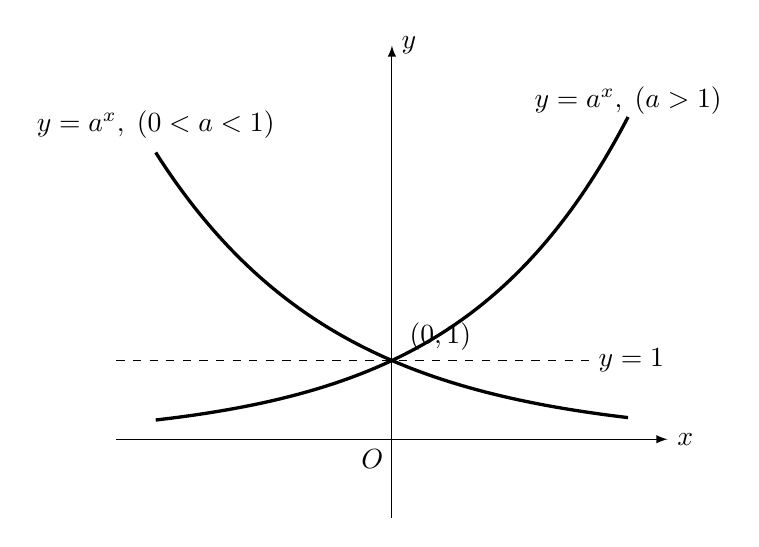
\begin{tikzpicture}[>=latex]
\draw[->](-3.5,0)--(3.5,0)node[right]{$x$};
\draw[->](0,-1)--(0,5)node[right]{$y$};
\draw[dashed] (-3.5,1)--(2.5,1)node[right]{$y=1$};
\draw [domain=-3:3, samples=100, very thick]plot(\x, {1.6^(\x)});
\draw [domain=-3:3, samples=100, very thick]plot(\x, {0.65^(\x)});
\node at (-3,4){$y=a^x,\; (0<a<1)$};
\node at (3,4.3){$y=a^x,\; (a>1)$};
\node at (-.25,-.25){$O$};
\node at (.1,1.3)[right]{$(0,1)$};
\end{tikzpicture}
  \caption{}\label{fig:4-10-3}
\end{figure}

\begin{Theorem}{逆定理}
  任何一个满足上述性质 1 和 2 的函数 $f(x)$ 必定是一个指数函数,其底为 $a=f(1)$。
\end{Theorem}
 
\begin{proof}
由性质 1, 对于任何实数 $x$,有
\[f(0)f(x)=f(0+x)=f(x)\]
即得,$f(0)=1$。 当 $f(x)$ 递增时,$f(1)=a>f(0)=1$,而当 $f(x)$ 递减时,$f(1)=a<f(0)=1$。

由性质 1:
\[\begin{split}
  f(m)&=f\big((m-1)+1\big)=f(m-1)\cdot f(1)\\
  &=f(m-2)\cdot \big(f(1)\big)^2=f(m-3)\cdot \big(f(1)\big)^3\\
  & \cdots  \\
  & =\big(f(1)\big)^m=a^m
\end{split}\]
又因为
\[\begin{split}
  \left[f\left(\frac{m}{n}\right)\right]^n&=f\overbrace{\left(\frac{m}{n}+\frac{m}{n}+\cdots +\frac{m}{n}\right)}^{n\text{个}}\\
  &=f(m)=a^m
\end{split}\]
所以:$f\left(\dfrac{m}{n}\right)=\sqrt[n]{a^m}=a^{\tfrac{m}{n}}$

因为 $f\left(\dfrac{m}{n}\right)f\left(-\dfrac{m}{n}\right)=f\left(\dfrac{m}{n}-\dfrac{m}{n}\right)=f(0)=1$

所以$f\left(-\dfrac{m}{n}\right)=\dfrac{1}{f\left(\dfrac{m}{n}\right)}=\dfrac{1}{a^{\tfrac{m}{n}}}=a^{-\tfrac{m}{n}}$

所以,$f(r)=a'$,对于正、负分数$r$都成立。

再由单调性,和实指数幂的定义,就可以说明 $f(x)=a^x$ 对于任何实数都成立。

设 $x\in\mathbb{R}$ 为一任意实数,$r_n\to x\leftarrow s_n$ 是 $x$ 的左、右夹逼有理数列,即
\begin{equation}
  \label{eq:pinch_sequence}
  r_1\leqslant r_2\leqslant\cdots \leqslant r_n\leqslant\cdots \leqslant x\leqslant\cdots \leqslant s_n\leqslant\cdots \leqslant s_2\leqslant s_1
\end{equation}
并且 $\lim(s_n-r_n)=0$。

由不等式 \eqref{eq:pinch_sequence} 和 $f(x)$ 的递增性(递减性),得到
\begin{equation}
  \label{eq:pinch_function}
  f(r_1)\leqslant f(r_2)\leqslant\cdots \leqslant f(r_n)\leqslant\cdots \leqslant f(x)\leqslant\cdots \leqslant f(s_n)\leqslant\cdots \leqslant f(s_2)\leqslant f(s_1)
\end{equation}
$r_n,s_n$ 都是有理数。
(若 $f(x)$ 递减,我们得到不等式 \eqref{eq:pinch_function} 的反向不等式)。

不等式 \eqref{eq:pinch_function} 可改写成
\begin{equation}
  \label{eq:pinch_function2}
  a^{r_1}\leqslant a^{r_2}\leqslant\cdots \leqslant a^{r_n}\leqslant\cdots \leqslant a^{x}\leqslant\cdots \leqslant a^{s_n}\leqslant\cdots \leqslant a^{s_2}\leqslant a^{s_1}
\end{equation}
而上节实数指数定义中,$a^x$ 是唯一能满足 \eqref{eq:pinch_function2} 的实数,所以 $f(x)=a^x$。

在上面的讨论中,$x$ 是一个任意的实数,因此,$f(x)=a^x$,对于任何实数 $x$ 恒成立。
\end{proof}

\begin{example}\label{eq:exponential_inequality}
设 $a,b$ 是不等的正实数,试证
\[a^ab^b>(ab)^{\tfrac{a+b}{2}}>a^bb^a\]
\end{example}

\begin{proof}
不妨设 $a>b$,则 $\dfrac{a}{b}>1$,$a-b>0$。于是,根据实指数幂性质 1,可得:
\[\frac{a^ab^b}{(ab)^{\tfrac{a+b}{2}}}=a^{\tfrac{a-b}{2}}\cdot b^{\tfrac{b-a}{2}}=\left(\frac{a}{b}\right)^{\tfrac{a-b}{2}}>1\]

由于 $a>0,\;  b>0\Rightarrow ab>0$,因此,$(ab)^{\tfrac{a+b}{2}}>0$,所以,有
\[a^ab^b>(ab)^{\tfrac{a+b}{2}}\]
另外,根据同样的道理,有
\[\frac{(ab)^{\tfrac{a+b}{2}}}{a^bb^a}=a^{\tfrac{a-b}{2}}\cdot b^{\tfrac{b-a}{2}}=\left(\frac{a}{b}\right)^{\tfrac{a-b}{2}}>1\]
又 $a^b>0$,$b^a>0$。 所以 $(ab)^{\tfrac{a+b}{2}}>a^b b^a$,这就证明了
\[a^ab^b>(ab)^{\tfrac{a+b}{2}}>a^b b^a\]
\end{proof}

\begin{Exercise}
\begin{question}
  \item 利用实指数幂的性质,指出下列不等式中,$a$ 是大于 1, 还是大于 0 而小于 1?
  \begin{tasks}(2)
    \task $a^{\sqrt{2}}<a^{\tfrac{\sqrt{2}}{2}}$
    \task $a^{-\sqrt{3}}>a^2$
    \task $a^{-\sqrt{5}-\sqrt{7}}>a^{-5}$
    \task $a^{1+\sqrt{5}}<a^{2+\sqrt{2}}$
    \task $a^{\sqrt{7}+\sqrt{2}}<a^{\sqrt{6}+\sqrt{3}}$
  \end{tasks}
  \item 作下列各函数的图象:
  \begin{tasks}(2)
    \task $y=3^x$
    \task $y=3^{-x}$
  \end{tasks}
  \item 
  \begin{tasks}
    \task 证明 $f(x)=\dfrac{2^x+2^{-x}}{2}$ 是偶函数,并作出它的图象;
    \task 当 $x$ 为何值时,$f(x)$ 有最小值,并求最小值。
  \end{tasks}
  \item 设 $a,b,c$ 是不等的正数,证明:
  \begin{tasks}
    \task $a^{2 a} b^{2 b} c^{2 c}>a^{b+c} b^{c+a} c^{a+b}$
    \task $a^{a} b^{b} c^{c}>(a b c)^{\tfrac{a+b+c}{3}}$
  \end{tasks}
  (提示:利用\cref{eq:exponential_inequality} 的结果)
  \item 证明:
  \begin{tasks}
    \task 当 $n$ 是 1 或不小于 5 的自然数时,总有 $2^n>n^2$;
    \task $\lim\limits_{n\to\infty}\dfrac{2^n}{n}=\infty$。
  \end{tasks}
\end{question}
\end{Exercise}

\section{对数函数}

由实数幂的定义,我们得知指数函数
\[a^x,\quad (a>0,\;a\ne 1),\qquad x\in\mathbb{R}\]
的值都是正的,现在还要进一步说明指数函数的值域是正实数集,也就是必须证明下面的命题。

\begin{Theorem}{命题}
给定不等于 1 的正实数 $a$,对于任意正数 $b$,一定存在唯一的一个实数 $c$,满足下列方程
\[a^c=b\]
\end{Theorem}

\begin{proof}
为确定起见,设 $a>1$,依实指数函数的性质 5,$\lim\limits_{x\to-\infty}a^x=0$,可以找出这样一数 $c_1$ 以使 $a^{c_1}<b$,依 $a^x,\;(a>1)$ 是增函数且$\lim\limits_{x\to+\infty}a^x=+\infty$,可以找出这样的数 $c_2>c_1$,以使 $a^{c_2}>b$,现在由连续函数中间值定理知道,在 $c_1$ 与 $c_2$ 之间有实数 $c$ 以使 $a^c=b$,再由单调性知道这个数是唯一的。类似地可以证明 $0<a<1$ 的场合,这个证明留给同学补全。
\end{proof}


现在我们根据第八章第五节反函数定理可以说由指数函数得到一个定义在正实数变域上的反函数,称为对数函数,记作 $f:\mathbb{R}^+\mapsto \mathbb{R}$,这里 $f(x)=\log_a x$,它是连续的单调函数。正式定义如下:

\begin{Definition}
若 $a>0$ 且 $a\ne 1$,那么 $y=\log_a x$,当且仅当 $x=a^y$。我们称 $y$ 是以 $a$ 为底的对数,函数 $f:\mathbb{R}^+\mapsto \mathbb{R}$,这里 $f(x)=\log_a x$ 称为\Concept{对数函数}。
\end{Definition}

这个定义导致下面有用的结果:
\begin{enumerate}[itemsep=5pt]
  \item $a^{\log_a x}=x,\qquad \log_a a^x=x$
  \item $\log_a (xy)=\log_a x+\log_a y$
  \item $\log_a \dfrac{x}{y}=\log_a x-\log_a y$
  \item $\log_a x^r=r\log_a x$
  \item $\log_a b=\dfrac{\log_c b}{\log_c a}$(换底公式)。
\end{enumerate}
证明过程请看第三册第一章。

从函数的图象来说:$y=\log_a x,\; (x\in\mathbb{R})$ 的图象能由 $y=a^x,\; (x\in\mathbb{R})$ 的图象经 $y=x$ 的反射而得到,如\cref{fig:4-10-4}。
\begin{figure}
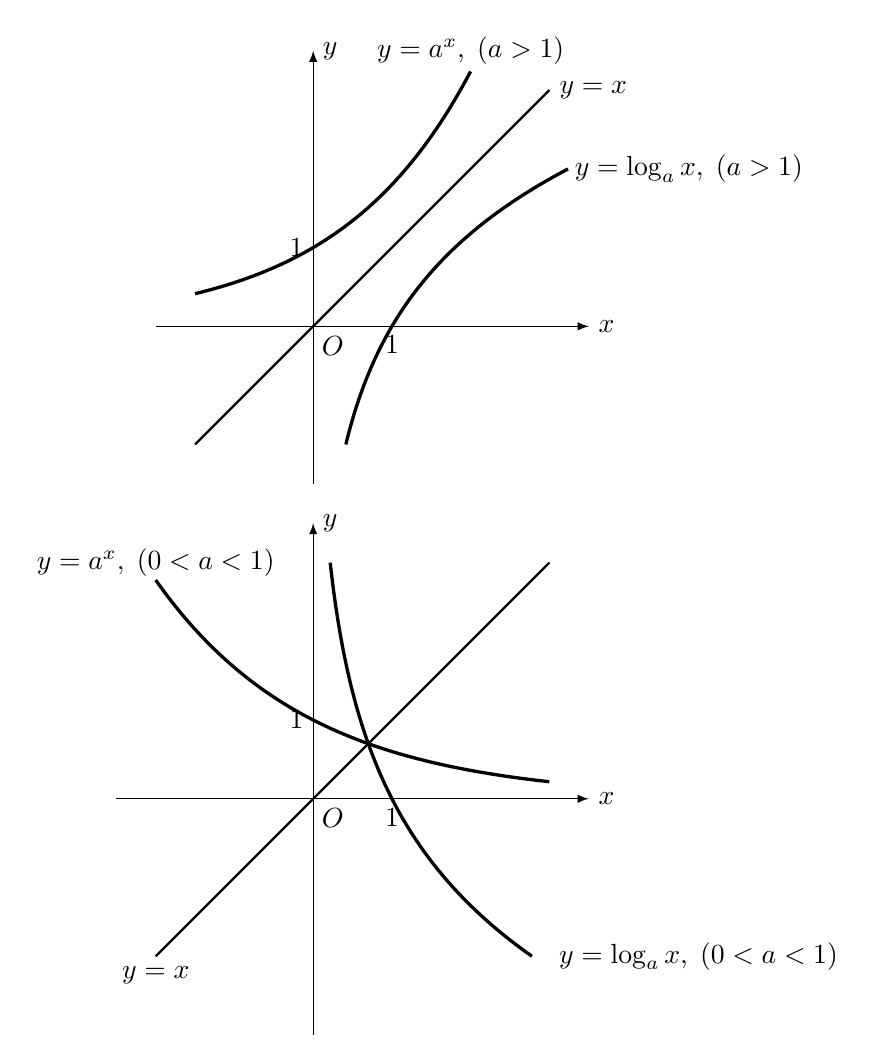
\begin{tikzpicture}[>=latex]
\begin{scope}
  \draw[->](-2,0)--(3.5,0)node[right]{$x$};
\draw[->](0,-2)--(0,3.5)node[right]{$y$};
\draw[thick] (-1.5,-1.5)--(3,3)node[right]{$y=x$};
\draw[domain=-1.5:2, samples=100, very thick]plot(\x,{1.8^(\x)});
\draw[domain=-1.5:2, samples=100, very thick]plot({1.8^(\x)},\x);
\node at (2,3.5){$y=a^x,\; (a>1)$};
\node at (3.2,2)[right]{$y=\log_a x,\; (a>1)$};
\node at (1,0)[below]{1};
\node at (0,1)[left]{1};
\node at (.25,-.25){$O$};
\end{scope}
\begin{scope}[yshift=-6cm]
  \draw[->](-2.5,0)--(3.5,0)node[right]{$x$};
  \draw[->](0,-3)--(0,3.5)node[right]{$y$};
  \draw[thick] (-2,-2)node[below]{$y=x$}--(3,3);
  \draw[domain=-2:3, samples=100, very thick]plot(\x,{0.6^(\x)});
  \draw[domain=-2:3, samples=100, very thick]plot({0.6^(\x)},\x);
  \node at (-2,3){$y=a^x,\; (0<a<1)$};
\node at (3,-2)[right]{$y=\log_a x,\; (0<a<1)$};
\node at (1,0)[below]{1};
\node at (0,1)[left]{1};
\node at (.25,-.25){$O$};
\end{scope}
\end{tikzpicture}
  \caption{}\label{fig:4-10-4}
\end{figure}

由于 $x$ 轴是指数函数图象的渐近线,故 $y$ 轴是对数函数图象的渐近线。相应于指数函数的极限值:
\[\begin{split}
  \lim_{x\to -\infty} a^x=0&,\qquad a>1\\
  \lim_{x\to +\infty} a^x=0&,\qquad 0<a<1
\end{split}\]
有对数函数的极限值:
\[\lim_{x\to 0^+} \log_a x=\begin{cases}
  -\infty, & a>1\\
  +\infty ,& 0<a<1
\end{cases}\]

相应于指数函数的特征性质,也就有对数函数的特征性质:
\begin{enumerate}
  \item $\log_a (x_1\cdot x_2)=\log_a x_1+\log_a x_2$
  \item 单调性。当 $a>1$ 递增;当 $0<a<1$ 递减。
  \item 连续性。即在 $(0,+\infty)$ 内处处连续。同样地,对应于第三节中的定理,总结成下面的定理。
\end{enumerate}

\begin{Theorem}{定理}
对数函数 $f(x)=\log_a x$ 满足下列性质:
  \begin{enumerate}
    \item $f(x_1\cdot x_2)=f(x_1)+f(x_2)$
    \item 单调性。$a>1$ 时,递增;$0<a<1$ 时,递减。
    \item 在 $x>0$ 半直线上,处处连续。
  \end{enumerate}
\end{Theorem}
 
\begin{Theorem}{逆定理} 
  任何一个满足性质 1、2 的函数 $f(x) $一定是一个对数函数,即存在适当的 $a$,使得 $f(x)=\log_a x$。
\end{Theorem}

\begin{proof}
由性质 1,$f(x_1)=f(x_1\cdot 1)=f(x_1)+f(1)$。因此 $f(1)=f(x_1)-f(x_2)=0$。

我们先任取一常数 $A>1$,则由性质 2 知
\[f(A)\ne f(1)=0\]
再由性质 1
\[f(A^m)=\underbrace{f(A)+f(A)+\cdots+f(A)}_{\text{$m$项}}=mf(A),\qquad m\in\mathbb{N}\]

又
\[\begin{split}
  mf(A)&=f(A^m)=f\left(\left((A)^{\tfrac{m}{n}}\right)^n\right)\\
  &=\underbrace{f\left(A^{\tfrac{m}{n}}\right)+\cdots+f\left(A^{\tfrac{m}{n}}\right)}_{\text{$n$项}}=nf\left(A^{\tfrac{m}{n}}\right)
\end{split} \]
$\therefore\quad f\left(A^{\tfrac{m}{n}}\right)=\frac{m}{n}f(A),\qquad m,n\in\mathbb{N}$

又$\because\quad f\left(A^{\tfrac{m}{n}}\right)+f\left(A^{-\tfrac{m}{n}}\right)=f\left(A^{\tfrac{m}{n}}\cdot A^{-\tfrac{m}{n}}\right)=f(A^0)=f(1)=0$

$\therefore\quad f\left(-A^{\tfrac{m}{n}}\right)=-f\left(A^{\tfrac{m}{n}}\right)=-\frac{m}{n}f(A)$

\bigskip
综合上面所证,所以对于所有有理数 $r\in\mathbb{Q}$,都有
\[f(A^r)=rf(A)\]
从此不难用单调性和极限过程,导出
\begin{equation}
  \label{eq:logarithmic_function}
  f(A^{\beta })=\beta f(A),\qquad \beta \in\mathbb{R}
\end{equation}

令 $A^{\beta }=x$,则 $\beta =\log_A x$,于是\cref{eq:logarithmic_function} 可写成
\begin{equation}
  \label{eq:logarithmic_function2}
  f(x)=f(A)\cdot \log_A x
\end{equation}
这样我们得到一个连续的单调的对数型函数\cref{eq:logarithmic_function2}。为了化去常数因子 $f(A)$,我们要用一些技巧如下:令 $a=A^{\tfrac{1}{f(A)}}$,于是
\[1=\log_a a=\log_a A^{\tfrac{1}{f(A)}}=\frac{1}{f(A)}\cdot \log_a A\]
即:$f(A)=\log_a A$,代入\cref{eq:logarithmic_function2},得到:
\[f(x)=\log_A x\cdot \log_a A=\log_a x\]
\end{proof}

\begin{Exercise}
\begin{question}
  \item 求下列各函数的定义域与值域,如果它们是可逆的,写出以 $x$ 为自变数的反函数。
  \begin{tasks}(2)
    \task $y=\log_2(x-2)$
    \task $y=\log_2\dfrac{1}{x}$
    \task $y=e^{-x}$
    \task $y=\sqrt{\lg\cos2\uppi x}$
  \end{tasks}
  \item 计算下列各式的值:
  \begin{tasks}(2)
    \task $2^{\log_4 9}$
    \task $5^{\log_{0.2} 7}$
    \task $3^{\log_{\sqrt{2}}6}$
    \task $6^{1+\log_6 5}$
    \task $25^{\tfrac{1}{3} \log 5^{27}-\log_{5} 4}$
    \task $10^{\lg\sqrt{100}}$
    \task $\log _{\sqrt{4-\sqrt{15}}} \sqrt{4+\sqrt{15}}$
    \task $4-\lg 8-3 \lg 5$
    \task $ \lg ^{2} 5+\lg 2 \lg 50$
    \task $\dfrac{3 \lg 1728}{1+\dfrac{1}{2} \lg 0.36+\dfrac{1}{3} \lg 8}$
    \task $\log _{a} b \cdot \log _{b} c \cdot \log _{c} d$
    \task $\left(\log _{2} 3+\log _{4} 9\right)\left(\log _{3} 4+\log _{9} 2\right)$
  \end{tasks}
  \item 证明下面的恒等式:
  \begin{tasks}(2)
    \task $\log_a b=\dfrac{\log_c b}{\log_c a}$
    \task $\log_a b\cdot \log_b a=1$
    \task! $\dfrac{\log_a x}{\log_{ab} x}=1+\log_a b$  
    \task! \[\begin{split}
      &\quad \frac{1}{(\log_x 2)(\log_x 4)}+   \frac{1}{(\log_x 4)(\log_x 8)}+   \frac{1}{(\log_x 8)(\log_x 16)}+\cdots \\
      &+   \frac{1}{(\log_x 2^{n-1})(\log_x 2^n)}=\left(1-\frac{1}{n}\right)\left(\frac{1}{\log_x 2}\right)^2
    \end{split}\]
  \end{tasks}
  \item 
  \begin{tasks}
    \task 已知 $\lg2=a$,$\lg7=b$,求 $\log_8 9.8$;
    \task 已知 $\log_{18}9=a$,$\log_{18}5=b$,求 $\log_{36}45$;
    \task 已知 $\lg198=2.2966$,$\lg2=0.3010$,$\lg3=0.4771$,求 $\lg 11$;
    \task 已知 $\log_{12}7=m$,$\log_{12}3=n$,求 $\log_{18}63$。
  \end{tasks} 
  \item 已知 $\lg3=0.4771$,问 $\left(\dfrac{1}{3}\right)^{20}$ 表成小数时,不等于 0 的第一个有效数字出现在哪里?
  \item 证明下面不等式:
  \begin{tasks}
    \task $\left|\log _{a} b\right|+\left|\log _{b} a\right| \geqslant 2$
    \task $\dfrac{1}{\log _{2} \uppi}+\dfrac{1}{\log _{\uppi} 2}>2$
    \task 若 $a>b>0$ 且 $c>1$,则 $\log _{c} \dfrac{b}{a}<\log _{c} \dfrac{1+b}{1+a}$。
    \task 若 $t>-1$,$\varphi(t)=-\lg(1+t)$,则 $\varphi\left(\dfrac{t_{1}+t_{2}}{3}\right)<\dfrac{\varphi\left(t_{1}\right)+\varphi\left(t_{2}\right)}{2}$
  \end{tasks}
  \item 当 $2 x+5 y=20$ 时, 求 $\log _{2} x+\log _{2} y$ 的最大值。
  \item 设 $x>1$,$y>1$ 且 $2 \log _{x} y-2 \log _{y} x+3=0$,那么 $x^{2}-$ $4 y^{2}$ 的最小值是多少?
  \item 设 $x>2$,$y>2$,比较下列各式的大小:
  \[\log _{2} \frac{x+y}{2} ;\qquad \frac{1}{2} \log _{2}(x+y); \qquad \frac{1}{2}\left(\log _{2} x+\log _{2} y\right)\]
  \item  求证等比数列的各项的对数组成等差数列。
  \item  有等比数列, 它的公比为 2, 项数为10, 如果各项 取以2 为底的对数, 它们的和是 25, 求这等比数列的和。
  \item 试问数列
  $$\lg100,\; \lg\left(100\sin\frac{\uppi}{4}\right),\; \lg\left(100\sin^2\frac{\uppi}{4}\right),\; \ldots ,\; \lg\left(100\sin^{n-1}\frac{\uppi}{4}\right),\; \ldots$$
  的前多少项的和的值最大?并求出最大值(这里取 $\lg2=0.3010$)。
\end{question}
\end{Exercise}

\section{指数方程与对数方程}
指数中含有未知数的方程叫做\Concept{指数方程}。下面我们介绍几种常见的指数方程及其解法。

\subsection{可化为 \texorpdfstring{$\alpha^{f(x)}=\alpha^{g(x)}\; (a>0\text{\;且\;}a\neq 1)$}{} 的指数方程}
对于这类方程,我们根据指数函数的单调性得到 $\alpha^{f(x)}=\alpha^{g(x)}$ 成立的必要充分条件是 $f(x)=g(x)$。 因此,指数方程 $\alpha^{f(x)}=\alpha^{g(x)}$ 在 $a>0$ 且 $a\ne 1$ 的条件下就可以转化为代数方程 $f(x)=g(x)$ 来解。

\begin{example}
  解方程 $5^{-x}\cdot 50^x=\dfrac{1}{1000(10^{2x-1})^{-3}}$
\end{example}

\begin{solution}
原方程化简为 $(5^{-1}\cdot 50)^x=\dfrac{10^{6x-3}}{10^3}$,即:
\[10^x=10^{6x-6}\]

由于底数 $a=10>0$ 且 $\ne 1$,得到
\[x=5x-6 \quad \Rightarrow\quad x=\frac{6}{5}\]
所以原方程的解集是 $\left\{\dfrac{6}{5}\right\}$。
\end{solution}


\begin{example}
解方程 $17^{3x^2+x-2}=1$
\end{example}

\begin{solution}
$\because\quad 1=17^0$,原方程可写成
\[17^{3x^2+x-2}=17^{0}\]
于是根据指数函数的单调性,得到
\[3x^2+x-2=0\]
由此
\[x_1=\frac{2}{3},\qquad x_2=-1\]
所以 原方程的解集是 $\left\{-1,\dfrac{2}{3}\right\}$。
\end{solution}

\subsection{可化为形如 $a^{f(x)}=b^{g(x)}$ 的指数方程}
这里($a>0$,$b>0$,$a\ne 1$,$b\ne 1$),一般用两边取对数的方法来解。

\begin{example}
解方程 $17^x=300$
\end{example}

\begin{solution}
两边取常用对数,得到
\[\begin{split}
  x\lg17&=\lg300\\
  x&=\frac{\lg300}{\lg 17}\approx \frac{2.4771}{1.2304}\approx 2.0132
\end{split}\]  
\end{solution}  
  
\begin{example}
  解方程 $5^{2x}-7x-35\cdot 5^{2x}+35\cdot 7^x=0$
\end{example}

\begin{solution}
原方程化简为 $7^x (35-1)=5^{2x}(35-1)$

两边除以 34, 得到:$5^{2x}=7^x$

两边取常用对数
\[\begin{split}
  2x\lg5&=x\lg7\\
x(2\lg5-\lg7)&=0
\end{split} \]
$\because\quad   2\lg5-\lg7=\lg25-\lg7\ne 0,\qquad \therefore\quad x=0$

因此,原方程的解集是 $\{0\}$。
\end{solution}

\subsection{可化为一元二次方程的指数方程}

\begin{example}
解方程 $\left(\sqrt{2-\sqrt{3}}\right)^x+\left(\sqrt{2+\sqrt{3}}\right)^x=4$
\end{example}

\begin{solution}
注意到 $\sqrt{2-\sqrt{3}}\cdot \sqrt{2+\sqrt{3}}=\sqrt{4-3}=1$,原方程的两边乘以 $\left(\sqrt{2-\sqrt{3}}\right)^x$,得到
\[\left(\sqrt{2-\sqrt{3}}\right)^{2x}+1=4\left(\sqrt{2-\sqrt{3}}\right)^x\]
即
$\left(\sqrt{2-\sqrt{3}}\right)^{2x}-4\left(\sqrt{2-\sqrt{3}}\right)^x+1=0$

$\therefore\quad \left(\sqrt{2-\sqrt{3}}\right)^x=2+\sqrt{3}\quad \text{或}\quad \left(\sqrt{2-\sqrt{3}}\right)^x=2-\sqrt{3}$

即:
\[\left({2-\sqrt{3}}\right)^{\tfrac{x}{2}}=\left({2-\sqrt{3}}\right)^{-1}\quad \text{或}\quad \left({2-\sqrt{3}}\right)^{\tfrac{x}{2}}=2-\sqrt{3}\]
$\therefore\quad x=-2\quad \text{或}\quad x=2$

$\therefore\quad $原方程的解集是$\{-2,2\}$。
\end{solution}

未知数前面有对数符号的方程称为对数方程。解对数方程一般常用的方法是根据对数定义直接把对数式的等式写成指数形式的等式。也有时根据对数函数的单调性把对数方程化为代数方程来解。但是必须注意在解对数方程之前,应该先确定使方程中的对数都有意义的定义域,由此便确定了方程的根的上、下界。在求得对数方程之解后,应该舍去在根的上、下界之外的增根,换言之,把那些使真数或底数为非正数或使底数等于1的根舍去,下面介绍几种常见的对数方程。

\subsection{形如 $\log_{f(x)}g(x)=c$\; (其中 $c$ 是常数)的对数方程}

可以根据对数定义将它化为指数形式的等式去解。
\begin{example}
解方程 $\log_{x-5}(3x^2-16x+29)=2$
\end{example}

\begin{solution}
方程中的对数有意义必须
\[\begin{cases}
  x>5\quad\text{且}\quad  x-5\ne 1 \\
  13x^2-16x+29>0
\end{cases}\] 
根据对数定义得到
\[ 3x^2-16x+29=(x-5)^2\]
解得:$x_1=1,\qquad x_2=2$。

由于 1 和 2 都小于 5, 所以原方程没有解,即原方程的解集是空集。
\end{solution}

\begin{example}
解方程 $\log_3[3+2\lg(1+x)]=0$
\end{example}

\begin{solution}
根据对数定义得到 $3+2\lg(1+x)=1$,即:
\[\lg(1+x)=-1\]
再由对数定义有
\[\begin{split}
  1+x&=10^{-1}\\
  x&=-0.9
\end{split}\]  
经验算可知原方程的解集是 $\{-0.9\}$。
\end{solution}

\subsection{可以化成形如 $\log_a f(x)=\log_a g(x)$ 的对数方程}

由对数函数的单调性知道,上面方程成立的充分必要条件是
\[\begin{cases}
  f(x)>0\\
  g(x)>0\\
  f(x)=g(x)
\end{cases}\]
因此对数方程可化为代数方程和不等式来解。

\begin{example}
解方程 $\lg x+\lg(x^2-4)=\lg3+\lg(x+2)$
\end{example}

\begin{solution}
方程中的对数有意义,必须
\[\begin{cases}
  x>0\\
  x^2-4>0\quad \Rightarrow\quad  x>2\\
  x+2>0
\end{cases}\]
原方程化为 $\lg x(x^2-4)=\lg 3(x+2)$,由此得到
\[x(x^2-4)=3(x+2)\]
即:$(x-2)(x^2-2x-3)=0$,
解得:
\[x_1=2,\qquad x_2=-1,\qquad x_3=3\]
其中只有 $x_3=3>2$,所以原方程的解集是 $\{3\}$。
\end{solution}

根据指数函数与对数函数的单调性也可以解相应的一些不等式。由于作对数变形时,也有可能把原来数的定义域缩小了,这时就会丢掉解,因此,作对数变形时,应该避免这种情形发生。例如,解 $\lg x^2=1$,如果利用等式:$\lg x^2=2\lg x$,把原方程变形为 $2\lg x=1$,这时由这个方程只能解出 $x=\sqrt{10}$,丢失了原方程的一个根 $-\sqrt{10}$。

\begin{example}
  解不等式 $\log_{\tfrac{1}{3}}[\log_4 (x^2-5)]>0$
\end{example}

\begin{solution}
  原不等式等价于 $0<\log_4(x^2-5)<1$,由此 $1<x^2-5<4$,即:
\[6<x^2<9\]
$\therefore\quad \sqrt{6}<|x|<3$
从而:
\[\sqrt{6}<x<3\quad \text{或}\quad -3<x<-\sqrt{6}\]
\end{solution}

\begin{example}
  解 $\log_a x>6\log_x a-1,\qquad (0<a<1)$
\end{example}

\begin{solution}
  原不等式可写成
\begin{equation}
  \label{eq:inequality1}
  \log_a x>\frac{6}{\log_a x}-1
\end{equation}
分两种情形来解:
\begin{enumerate}
  \item 设 $0<x<1$,则 $\log_a x>0,\quad (0<a<1)$。
  
由\cref{eq:inequality1} 得 $\log_a^2 x+\log_a x-6>0$,由此得:
\begin{equation}
  \label{eq:solution1}
  \log_a x<-3
\end{equation}
或
\begin{equation}
  \label{eq:solution2}
  \log_a x>2
\end{equation}
由\cref{eq:solution1} 得 $x>\dfrac{1}{a^3}>1$,这与前设 $0<x<1$ 矛盾。所以\cref{eq:solution1} 无解。

由\cref{eq:solution2} 得 $0<x<a^2<1$,因此由\cref{eq:inequality1} 得:$0<x<a^2$

\item 设 $x>1$,则 $\log_a x<0,\quad (0<a<1)$。

由\cref{eq:inequality1} 得 $\log_a^2 x+\log_a x-6<0$,由此得:
\[-3<\log_a x<2\]
$\because\quad 0<a<1,\qquad \therefore\quad a^2<1<x<a^{-3}$

因此,由\cref{eq:inequality1} 可得,$1<x<\dfrac{1}{a^3}$。

$\therefore\quad $ 原不等式的解集是 $\left\{x|0<x<a^2\right\}\cup\left\{x\Big|1<x<\dfrac{1}{a^3}\right\}$
\end{enumerate}
\end{solution}

\begin{example}
  解不等式 $\dfrac{1}{\log_2 x}-\dfrac{1}{\log_2 x-1}<1$
\end{example}

\begin{solution}
  原不等式可化简为 $\dfrac{1+\log_2 x(\log_2 x-1)}{\log_2 x(\log_2 x-1)}>0$,即:
\[\frac{\left(\log_2 x-\frac{1}{2}\right)^2+\dfrac{3}{4}}{\log_2 x(\log_2 x-1)}>0\]
由此得:$\log_2 x(\log_2 x-1)>0$,因此:
\[\log_2 x<0\quad \text{或}\quad \log_2 x>1\]
即:$0<x<1\quad \text{或}\quad x>2$。

由此原不等式的解集是 $\{x|0<x<1\}\cup\{x|x>2\}$。
\end{solution}

\begin{example}
  求函数 $f(x)=\sqrt{\log_{\tfrac{1}{2}}\dfrac{x}{x^2-1}}$ 的定义域。
\end{example}

\begin{solution}
\[\begin{split}
  \text{函数$f$有意义}&\Longleftrightarrow \log_{\tfrac{1}{2}}\frac{x}{x^2-1}\text{有意义}\Longleftrightarrow \log_{\tfrac{1}{2}}\frac{x}{x^2-1}\geqslant 0\\
  &\Longleftrightarrow  0<   \frac{x}{x^2-1}\leqslant1    \Longleftrightarrow  \begin{cases}
    \dfrac{x}{x^2-1}>0\\ \dfrac{x^2-x-1}{x^2-1}\geqslant 0
  \end{cases}           \\
  &\Longleftrightarrow     \begin{cases}
    -1<x<0\quad \text{或}\quad x>1\\
    x<-1\quad \text{或}\quad \dfrac{1-\sqrt{5}}{2}<x<1\quad \text{或}\quad x>\dfrac{1+\sqrt{5}}{2}
  \end{cases}               \\
  &\Longleftrightarrow   \begin{cases}
    -1<x<0\\  \dfrac{1-\sqrt{5}}{2}<x<1
  \end{cases}      \text{或}\quad  \begin{cases}
    x>1\\x>\dfrac{1+\sqrt{5}}{2}
  \end{cases}           \\
  &\Longleftrightarrow    \dfrac{1-\sqrt{5}}{2}<x<1  \quad \text{或}\quad   x>\frac{1+\sqrt{5}}{2}   \\
\end{split}\]
故函数 $f$ 的定义域为
\[\left\{x\Big| \frac{1-\sqrt{5}}{2}<x<1 \right\}\bigcup\left\{x\Big|x>\frac{1+\sqrt{5}}{2}  \right\}\]
\end{solution}


\begin{example}
  解方程 $\log_{\sin 3x}(\cos x-\cos2x)=1$
\end{example}

\begin{solution}
  要使方程中的对数有意义,$x$ 必须满足条件:
\begin{equation}
  \begin{cases}
    \sin 3x>0\quad \text{且}\quad \sin3 x\ne 1\\
    \cos x-\cos2x>0
  \end{cases}
\end{equation}
由原方程得 $\cos x-\cos2x=\sin3x$,即:
\[\sin \frac{3x}{2}\left(\sin \frac{x}{2}-\cos\frac{3x}{2}\right)=0\]
由此得:
\[\sin\frac{3x}{2}=0\quad \text{或}\quad \sin \frac{x}{2}-\cos\frac{3x}{2}=0\]
因为 $\sin\dfrac{3x}{2}=0$的解,根据$\sin3x=2\sin\dfrac{3x}{2}\cos\dfrac{3x}{2}$,知道一定也使 $\sin 3x=0$ 成立,而这与 $x$ 满足的条件:$\sin3x>0$
不合,因此,方程 $\sin\dfrac{3x}{2}=0$ 的解应该舍去。

由$\sin \dfrac{x}{2}-\cos \dfrac{3x}{2}=0$,得:
\[\sin \frac{x}{2}=\sin \left(\frac{\uppi}{2}-\frac{3x}{2}\right)\]
根据两角正弦相等条件,有
\[\frac{x}{2}=\frac{\uppi}{2}-\frac{3x}{2}+2k\uppi\quad \text{或}\quad \frac{x}{2}=\frac{\uppi}{2}+\frac{3x}{2}+2k\uppi\]
即:
\begin{equation}
x=\frac{\uppi}{4}+k\uppi
\end{equation}
或
\begin{equation}
  x=-\frac{\uppi}{2}-2k\uppi
\end{equation}
在单位圆上,分别作出(10.11)中和(10.12)中的诸角的终边,如\cref{fig:4-10-5}。

\begin{figure}[htp]
  \centering
\begin{tikzpicture}[>=latex]
\begin{scope}
  \draw[->] (-2,0)--(2,0)node[right]{$x$};
  \draw[->] (0,-1.5)--(0,2)node[right]{$y$};
\draw[thick] (0,0) circle (1);
\draw[very thick,->] (1,0) arc (0:180+45:1);
\draw[thick, <->] (45:1)node[above]{$\dfrac{\uppi}{4}$}--(180+45:1)node[below]{$\dfrac{5\uppi}{4}$};
\node at (.25,-.25){$O$};
\node at (1.4,0)[below]{$(1,0)$};
\node at (0,-2.2){$x=\dfrac{\uppi}{4}+2k\uppi$};
\end{scope}
\begin{scope}[xshift=5cm]
  \draw[->] (-2,0)--(2,0)node[right]{$x$};
  \draw[->] (0,-1.5)--(0,2)node[right]{$y$};
  \draw[thick] (0,0) circle (1);
\draw[very thick,->] (1,0) arc (0:-90:1);
\draw[thick, ->] (0,0)--(-90:1);
\node at (-.25,-.25){$O$};\node at (1.4,0)[below]{$(1,0)$};
\node at (0,-2.2){$x=-\dfrac{\uppi}{2}+2k\uppi$};
\end{scope}
\end{tikzpicture}
  \caption{}\label{fig:4-10-5}
\end{figure}

显然(10.11)又可写成
\begin{equation}
  x=\frac{\uppi}{4}+2k\uppi
\end{equation}
和
\begin{equation}
  x=\frac{5\uppi}{4}+2k\uppi
\end{equation}
再由(10.12), (10.13), (10.14)容易看出角 $3x$ 与角 $-\dfrac{3\uppi}{2}$,$\dfrac{3\uppi}{4}$ 和 $-\dfrac{\uppi}{4}$ 有相同的终边,所以若将式(10.12)和式(10.14)代入 $\sin3x$ 中,便得到
\[\begin{split}
  \sin 3\left(-\frac{\uppi}{2}-2k\uppi\right)&=\sin\left(-\frac{3\uppi}{2}\right)=-\sin\frac{3\uppi}{2}=1\\
  \sin 3\left(\frac{5\uppi}{4}+2k\uppi\right)&=\sin\frac{15\uppi}{4}=\sin\left(4\uppi-\frac{\uppi}{4}\right)=\sin\left(-\frac{\uppi}{4}\right)=-\frac{\sqrt{2}}{2}<0
\end{split}\]
因此这两组解是增解,应该舍去,经检验知 $x=\frac{\uppi}{4}+2k\uppi$ 满足不等式组, 所以方程的解集是 $\left\{x\Big|x=\dfrac{\uppi}{4}+2k\uppi,\quad k\in\mathbb{Z}\right\}$。

\end{solution}

\begin{Exercise}
\begin{question}
  \item 解下列各指数方程:
  \begin{tasks}(2)
    \task $\displaystyle 3^{2 x-1}=81$
    \task $\displaystyle \sqrt{5^{x}}=\sqrt[3]{25}$
    \task $\displaystyle \sqrt[4]{7^{x}}=\sqrt[5]{343}$
    \task $\displaystyle \sqrt[4]{a^{x+1}}=\sqrt[3]{a^{x-3}}$ $(a>0,\;  a \neq 1)$
    \task $\displaystyle \sqrt{2^{x}} \sqrt{3^{x}}=36$
    \task $\displaystyle \left(\frac{3}{4}\right)^x=\left(\frac{4}{3}\right)^5$
    \task $\displaystyle \left(\frac{4}{9}\right)^{4}=\left(\frac{3}{2}\right)^{x}$
    \task $\displaystyle \left(\frac{2}{3}\right)^{x}\left(\frac{9}{8}\right)=\frac{27}{64}$
    \task $\displaystyle  4^{\sqrt{x+1}}=64 \cdot 2^{\sqrt{x+1}} $
    \task $\displaystyle (0.25)^{x-2}=\frac{256}{2^{x+3}}$
    \task $\displaystyle \left(\frac{4}{9}\right)^{x}\left(\frac{27}{8}\right)^{x-1}=\frac{2}{3}$
    \task $\displaystyle 2^{x} \cdot 5^{4}=0.1\left(10^{x-1}\right)^{5}$
  \end{tasks}
  \item  解下列各指数方程:
  \begin{tasks}(2)
    \task  $3^{x+2}+3^{x-1}=28$
    \task  $5^{x+1}-5^{x-1}=24$
    \task  $3^{2 x-1}+3^{2 x-2}-3^{2 x-4}=315$
    \task  $3^{x}+3^{x+1}+3^{x+2}=5^{x+1}+5^{x+2}$
    \task  $4^{x}+2^{x+1}=80$ 
    \task  $ 3^{x+2}+9^{x+1}-810=0$
    \task  $3^{2 x+5}=3^{x+2}+2$
    \task  $3^{4 \sqrt{x}}-4.3^{2 \sqrt{x}}+3=0$
    \task  $4.9^{\sqrt{x}-2}-3.15^{\sqrt{x}-2}=25^{\sqrt{x}-2} $
    \task  $4^{2 x}-2.18^{2 x}=3.81^{28} $
    \task! $\left(\sqrt{5+2 \sqrt{6}}\right)^{x}+\left(\sqrt{5-2 \sqrt{6}}\right)^{x}=\dfrac{10}{3}$
  \end{tasks}
  \item  求最小整数指数 $x$,使
  \begin{tasks}(2)
    \task $\displaystyle \left(\frac{4}{5}\right)^{x}<0.000001$
    \task $\displaystyle \left(\frac{3}{5}\right)^{x}<0.0001$
    \task $\displaystyle \left(\frac{10}{9}\right)^{x}>1000000$
    \task $\displaystyle \left(\frac{4}{5}\right)^{x}>10000000$
  \end{tasks}
  \item  解下列各不等式
  \begin{tasks}(2)
    \task  $\displaystyle 3^{3-5 x}-\frac{1}{81}>0$
    \task  $\displaystyle (0.3)^{2 x^{2}+5 x+2}<1$
    \task  $\displaystyle 8^{x}+16^{\tfrac{3}{4} x+1}<34$
    \task  $\displaystyle \frac{(0.5)^{3 x^{2}+10 x+6}}{100}<0.00125$
    \task  $\displaystyle 2^{x+1} \cdot 5^{2 x-3}<\frac{24}{25}$
    \task  $\displaystyle 5^{2x}-30.5^{x}+125<0$
    \task  $\displaystyle 2^{3 x}-2^{x+1}<2^{3} $
    \task  $\displaystyle \frac{1}{\left(\dfrac{1}{10}\right)^{y}-1} \leqslant \frac{2}{\left(\dfrac{1}{100}\right)^{y}-10}$
    \task  $\displaystyle \frac{1}{2^{x}-1} \geqslant \frac{1}{4^{x}-3}$
    \task  $\displaystyle \left(\frac{3}{4}\right)^{x-2}\left(\frac{4}{3}\right)^{\tfrac{1}{x}}>\frac{9}{16}$
  \end{tasks}
  \item  解下列各对数方程:
  \begin{tasks}(2)
    \task  $\lg x=2-\lg 5$
    \task  $\dfrac{2\lg x}{\lg(5x-4)}=1$
    \task  $\dfrac{\lg x}{1-\lg x}=2$
    \task  $\log_{x-1}(x^2-5x+10)=2$
    \task  $2 \lg x=-\lg \left(6-x^{2}\right)$
    \task  $\dfrac{1}{5-\lg x}+\dfrac{1}{1+\lg x}=1$
    \task  $0.5 \lg (2 x-1)+\lg \sqrt{x-9}=1$
    \task  $\log _{2} \log _{3} \log _{4} x=0$
    \task  $\lg 9^{-1}+x \lg \sqrt[3]{3^{5 x-7}}=0$
    \task  $\lg 10^{\lg\left(x^{2}+21\right)}-1=\lg x$
    \task! $\lg(x+6)-\dfrac{1}{2}\lg(2x-3)=2-\lg 25$
  \end{tasks}
  \item 解下列各对数方程:
  \begin{tasks}(2)
    \task   $\displaystyle 2 \log _{4} x+2 \log _{x} 4=5$ 
    \task   $\displaystyle \log _{2}(x-1)^{2}-\log _{0.5}(x-1)=9$
    \task   $\displaystyle \log _{8} x+\log _{4} x+\log _{2} x=7$
    \task   $\displaystyle \log _{x}\left(5 x^{2}\right) \cdot\left(\log _{5} x\right)^{2}=1$
    \task   $\displaystyle \sqrt{\log _{x} \sqrt{3 x}} \cdot \log _{3} x=-1$
    \task   $\displaystyle \log _{3 x}\left(\frac{3}{x}\right)+\log _{3}^{2} x=1$
    \task   $\displaystyle \frac{\lg\left(\sqrt{x+1}+1\right)}{\lg\sqrt[3]{x-40}}=3$
    \task!  $\displaystyle \sqrt{\log _{x} 5 \sqrt{5}+\log _{\sqrt{5}} 5 \sqrt{5}} \cdot \log _{\sqrt{5}} x=-\sqrt{6}$
  \end{tasks}
  \item 解下列各方程:
  \begin{tasks}(2)
    \task $(0.4)^{\lg^2 x+1}=(6.25)^{2-\lg x^3}$
    \task $x^{\lg x+2}=1000$
    \task $\sqrt{x^{\lg \sqrt{x}}}=10$
    \task $\lg x+\lg \sqrt[3]{x}+\lg  \sqrt[9]{x}+\cdots=3$
    \task! $\lg 2+\lg \left(4^{x-2}+9\right)=1+\lg \left(2^{x-2}+1\right)$
    \task! $\log _{2}\left(9^{x-1}+7\right)=2+\log _{2}\left(3^{x-1}+1\right)$
    \task! $\log _{9} x+\left(\log _{9} x\right)^{2}+\left(\log _{9} x\right)^{3}+\cdots=1$,
    \task! $ 1+\log _{x} \frac{4-x}{x}=(\operatorname{lglg} n-1) \log _{x} 10$
  \end{tasks}
  \item 解下列各方程组:
  \begin{tasks}(2)
    \task  $\begin{cases}2^{\sqrt{{x}}+\sqrt{y}}=512 \\ \lg \sqrt{x y}=1+\lg 2\end{cases}$
    \task  $\begin{cases}\log _{x} \log _{2} \log _{x} y=0 \\ \log _{y} 9=1\end{cases}$
    \task  $\begin{cases}2^{\tfrac{x-y}{2}}-2^{\tfrac{x-y}{4}}=2 \\ 3^{\lg(2 y-x)}=1\end{cases}$
    \task  $\begin{cases}x y=40 \\ x^{12 y}=4,\end{cases}$
    \task  $\begin{cases}3.2^{x}-\log _{2} y=2 \\ 2^{x} \cdot \log _{2} y=1\end{cases}$
    \task  $\begin{cases}7^{y} \cdot \log _{5} x=2 \\ 4.7^{y}+\log _{5} x=2\end{cases}$
    \task  $\begin{cases}\lg^2x+\lg^2y=5\\ \lg x-\lg y=1\end{cases}$
    \task 求 $\begin{cases} x^{x+y}=y^{12}\\ y^{x+y}=x^3 \end{cases}$ 的整数解
  \end{tasks}
  \item 解下列各不等式:
  \begin{tasks}(2)
    \task  $\lg x>3$
    \task  $\lg (-x)>3$
    \task  $\lg x^2>3$
    \task  $\lg^2 x>3$
    \task  $\lg x<2\lg x$
    \task  $\lg x>2\lg x$
    \task  $\log_{\tfrac{1}{2}}(3x-5)<3$
    \task  $\lg x+\lg (x-3)>1$
    \task  $\lg (4x^2-9)>\lg (2x-3)+2$
    \task  $\lg (3-x)-1>\lg (2-x)$    
    \task  $\log_{\sqrt{0.5}}(26x)>\log_{\sqrt{0.5}}(5x^2+5)$
    \task  $x^{\log_a x+1}>ax^2,\quad (a>1)$
    \task! $\log_{\sqrt{2}}(x^2-2x+8)+2\sqrt{\log_2(x^2-2x+8)}\geqslant 12$
  \end{tasks}
  \item 求解
  \begin{tasks}
    \task 试求满足不等式 $2(\log_{0.5}x)^2+9\log_{0.5}x+9\leqslant 0$ 的 $x$ 的范围;
    \task $x$ 在 1 中求得的范围内变动时,试求 $f(x)=\left(\log_2 \dfrac{x}{3}\right)\left(\log_2 \dfrac{x}{4}\right)$ 的最大值 $M$ 和最小值 $L$。
  \end{tasks}
  \item 解下列方程:
  \begin{tasks}(2)
    \task $\displaystyle \log_{\sqrt{2}\sin x}(1+\cos x)=2$
    \task $\displaystyle \log_{\frac{1}{8\cos^2 x}}\sin x=\frac{1}{2}$
    \task $\displaystyle \frac{2}{\lg\left(\frac{1}{2}+\cos^2 x\right)}=\log_{\sin 2x}10$
    \task $\displaystyle \arcsin(\lg x)=0$
    \task $\displaystyle \lg(\arcsin x)=0$
    \task $\displaystyle \arccos(\uppi\log_3\tan x)=0$
  \end{tasks}
\end{question}
\end{Exercise}
\appendix 
\end{document}